\documentclass[11pt,a4paper]{article}
\usepackage{fontspec}
\usepackage[french]{babel}
\usepackage{amsmath,amssymb}
\usepackage[margin=2.3cm]{geometry}
\usepackage{booktabs,longtable,tabularx,array}
\usepackage{graphicx}
\usepackage{enumitem}
\usepackage{xcolor}
\usepackage{microtype}
\usepackage{url}
\usepackage{hyperref}

\hypersetup{colorlinks=true,linkcolor=blue!45!black,urlcolor=blue!45!black}
\setlist{nosep}
\newcommand{\code}[1]{\texttt{#1}}
\newcommand{\NW}{\mathrm{NW}}
\newcommand{\E}{\mathbb{E}}
\graphicspath{{../figures/}}

\title{Étude de sensibilité du modèle de société de crédit M4B\\
\large Rapport final : cartographie des paramètres, robustesse des
signatures, recommandations de réduction et feuille de route M5}
\author{Campagne \code{recherche/sensibilite\_m4b}}
\date{18 juillet 2026}

\begin{document}
\maketitle

\begin{abstract}
Nous cartographions la sensibilité du modèle multi-agents de société de
crédit M4B à ses cinq paramètres publics — intensité des naissances
$\lambda$, dépréciation $\delta$, volatilité $\sigma$, capital de
naissance $K_0$, taille d'échantillon du marché $k$ — sur 594
simulations tracées (exploration à trois graines, confirmation
indépendante à cinq graines et horizon doublé). Trois résultats
structurent la carte. (1)~\emph{Un seul régime} : dans tout l'espace
exploré ($\delta\in[0{,}01;0{,}10]$, $\sigma\in[0;1]$,
$K_0\in[2;200]$, $k\in[2;10]$, $\lambda\in[1;100]$), la dynamique est
stationnaire ; l'extinction n'existe que comme échec d'amorçage de
probabilité $e^{-\lambda}$ au premier pas, et le garde-fou de
population n'a jamais été atteint. (2)~\emph{Partage net des rôles} :
$\sigma$ gouverne la démographie et l'exposition ; $k$ gouverne les
inégalités et la statistique fine des avalanches ; $K_0$ est un levier
démographique log-linéaire ; $\delta$ agit essentiellement comme
l'échelle du capital, sauf dans le régime faiblement bruité
$\sigma<0{,}15$ où il module la propagation ; $\lambda$ est un pur axe
de taille finie (grandeurs intensives stables à $\pm1$--$2\,\%$).
(3)~\emph{Signatures robustes} : les tailles d'avalanches suivent
partout une loi de puissance tronquée (rapport de vraisemblance
$p\approx0$ contre la loi pure, log-normale battue à
$\lambda=100$) dont la coupure croît avec la taille du système
($\hat s_c\propto\lambda^{1{,}5}$ entre $\lambda=10$ et $30$, hors de
portée à $\lambda=100$) et dont l'exposant tronqué converge vers
$\alpha\simeq2{,}31$ ; le rapport de branchement reste épinglé à
$b\simeq0{,}30$ hors de la zone de transition $\sigma\lesssim0{,}2$,
qui relie continûment ce plateau au régime corrélé sans choc
($b=0{,}647$, $\alpha=1{,}80$). L'examen dédié de la valeur nette
$\NW=K+C-D$ — variable d'état de la mortalité — montre que
l'inégalité du modèle réside dans les bilans et non dans le capital
(Gini de $\NW$ $0{,}44$ contre $0{,}07$ au centre, avec des réponses
paramétriques opposées), que la position nette de crédit suit un cycle
de vie débiteur$\to$créancier, que la profondeur du trou
d'insolvabilité au décès, rapportée au capital par tête, est invariante
($-8{,}6\,\%$) le long de tous les axes d'échelle et ne dépend que de
$\sigma$, et que le canal de défaut de service est silencieux dans
toutes les plages étudiées : M4B y est une contagion de bilan pure.
L'analyse des cycles de l'activité
agrégée (production totale) montre des phases courtes, jamais plus
longues que le hasard (durées sous la référence géométrique, maxima de
10--13 pas), une volatilité de croissance en $\lambda^{-0{,}50}$ avec
un minimum intérieur vers $\sigma\simeq0{,}1$ séparant bruit endogène
(avalanches) et exogène (chocs), une asymétrie de krach — récessions
plus courtes et plus raides, skewness toujours négative, maximale dans
le régime corrélé — vivant à l'échelle des cascades, et un temps de
mémoire de l'activité verrouillé sur la durée de vie démographique
(corrélation de rang $0{,}93$).
Sur 168 contrastes testés en
confirmation, 141 sont confirmés, 19 sont des effets nuls cohérents,
3 gardent leur signe avec une amplitude décalée et 5 ne sont pas
confirmés — tous documentés (plus 182 contrastes d'extensions
post-audit — bilans et cycles — aux bilans détaillés dans les sections
correspondantes). Nous en déduisons des
recommandations prudentes de réduction pour le successeur M5 et une
feuille de route pour son étude analytique et la future mesure d'un
effet rebond.
\end{abstract}

\tableofcontents

\section{Introduction}

M4B est la réduction minimale validée du modèle de société de crédit
M4 : un moteur multi-agents où des entités naissent avec un capital
productif, subissent des chocs multiplicatifs, produisent de façon
concave, se prêtent un capital réel contre des créances nominales
perpétuelles, et meurent par défaut de service ou insolvabilité, en
propageant leurs pertes à leurs prêteuses (cascades). La présente étude
répond à quatre questions : quels paramètres contrôlent le régime
démographique, le réseau de crédit, les cascades et les distributions
individuelles ; où sont les non-linéarités et interactions ; quelles
signatures sont robustes aux graines, durées et fenêtres ; et quels
paramètres pourraient être réduits dans le successeur M5.

Le protocole complet (dictionnaire des métriques, plans, règles de
confirmation) a été figé avant les runs de production
(\code{protocole.pdf}, 17 juillet 2026) ; l'exploration est décrite
dans \code{rapport\_preliminaire.pdf}. Le présent rapport reprend
l'essentiel pour rester autonome, ajoute la phase confirmatoire et
conclut. Sauf mention contraire, chaque valeur est donnée avec sa
moyenne et son écart-type inter-graines, et provient de la phase
confirmatoire (cinq graines $\{11,\dots,15\}$, horizon $T=4000$,
fenêtre $[T/4,T]$).

\subsection{Le modèle en bref}
\label{sec:modele}

Chaque entité $i$ possède un capital réel $K_i\ge0$ (en joules).
Un pas de temps enchaîne : naissances
($B_t\sim\mathrm{Poisson}(\lambda)$, capital initial $K_0$) ; choc
multiplicatif i.i.d. $K_i\!\leftarrow\!K_ie^{\eta_i}$,
$\eta_i\sim\mathcal N(-\sigma^2/2,\sigma^2)$ (moyenne un) ; production
concave $K_i\!\leftarrow\!K_i+\sqrt{K_i}$ ; service des intérêts des
prêts perpétuels (défaut si le capital ne couvre pas le service dû) ;
dépréciation $K_i\!\leftarrow\!(1-\delta)K_i$ ; marché local du crédit
(un round par entité vivante : parmi $k$ entités tirées au hasard, la
plus riche prête à la plus pauvre vers la cible
$K^\ast=\sqrt{K_\ell K_b}$, au taux $r=\sqrt{r_\ell r_b}$ avec
$r_x=1/(2\sqrt{K_x})$) ; faillites en cascade (une morte annule ses
contrats, ses prêteuses perdent tout le principal exposé, son capital
résiduel est détruit ; les survivantes rendues insolvables meurent à la
génération suivante) ; mesures. Une \emph{avalanche} est une composante
connexe du graphe des pertes restreint aux mortes d'un même pas ; sa
taille $s$ est son nombre de mortes ; ses racines sont les faillites
initiales ; le rapport de branchement empirique est
$b=1-\sum_aR_a/\sum_aS_a$. La valeur nette est
$\NW_i=K_i+C_i-D_i$ (capital, créances, dettes).

\subsection{Campagne exécutée}

\begin{table}[tbh]
\centering
\begin{tabular}{@{}lrrrl@{}}
\toprule
Phase & Runs & Graines & $T$ & Rôle \\
\midrule
Benchmark & 6 & 0 & 2000 & coût, neutralité des mesures \\
Pilotes & 30 & 1--2 & 2000--8000 & audit des plages, contrôle temporel \\
Sondes de frontière & 16 & 1--2 & 2000 & $\sigma$ jusqu'à 1, $\delta=0{,}01$, $K_0\in\{2,200\}$ \\
OAT & 54$^{\ast}$ & 1--3 & 2000 & courbes par axe \\
Carte d'extinction & 42$^{\ast}$ & 1--3 & 2000 & $\lambda\in[1;10]\times\sigma\in\{0{,}25;0{,}5;1\}$ \\
Plan LHS & 192 & 1--3 & 2000 & screening global 64 points \\
Coupes 2D & 169$^{\ast}$ & 1--3 & 2000 & $\sigma\times k$, $\sigma\times\delta$ \\
Confirmation (lab) & 85 & 11--15/20 & 4000$^{\dagger}$ & 16 cellules, indépendante \\
\midrule
Total & 594 & & & 0 échec, 0 censure \\
\bottomrule
\end{tabular}
\caption{Campagne exécutée. $^{\ast}$après déduplication par
identifiant (une cellule partagée entre plans n'est simulée qu'une
fois) ; $^{\dagger}$2000 pour la cellule d'extinction $\lambda=2$.
Coût total $\approx22$\,h CPU, $8{,}6$\,Go. Moteur \code{m4b-mini-3},
condensat \code{f3a7ce02cd9185c7} ; parité M4/M4B vérifiée champ par
champ (unique recours à M4). Intégrité : résidu comptable relatif
maximal $6{,}8\cdot10^{-16}$, zéro erreur de carnet sur les 594 runs.}
\label{tab:campagne}
\end{table}

La table~\ref{tab:campagne} résume la campagne. Trois contrôles de
probité méritent mention : les options d'enregistrement ne changent pas
les trajectoires (séries bit à bit identiques sur deux contrôles) ; le
choix du burn-in ($T/8$, $T/4$ ou $T/2$) déplace la population moyenne
d'au plus $0{,}8\,\%$ en exploration ($4\,\%$ au pire sur les cellules
confirmatoires, atteint sur la petite population $\lambda=2$),
l'exposant $\hat\alpha$ d'au plus $0{,}08$ et $b$ d'au plus $0{,}011$ ;
et l'allongement de l'horizon ($T=4000$, et $8000$ sur le coin lent)
reproduit les valeurs de $T=2000$. Toutes les analyses fenêtrées
utilisent le burn-in $T/4$.

\section{Carte des régimes : un régime unique, deux artefacts évités}
\label{sec:regimes}

\paragraph{Fait central.} Aucune des 594 simulations n'a atteint le
garde-fou \code{pop\_max} ($30\,000$ entités) ni ne s'est éteinte après
s'être établie. Le diagnostic de censure exigé par le protocole est
donc \emph{sans objet} : aucune trajectoire n'a été censurée, et le mot
« explosion » du vocabulaire du moteur n'a jamais été employé pour
classer un run. Dans tout l'espace exploré —
$\delta\in[0{,}01;0{,}10]$, $\sigma\in[0;1]$, $K_0\in[2;200]$,
$k\in\{2,\dots,10\}$, $\lambda\in[1;100]$ — la population est
stationnaire (dérives relatives $\le4\,\%$ par fenêtre, demi-fenêtres
cohérentes) et les réponses varient continûment.

\paragraph{L'extinction est un artefact d'amorçage.} La population
initiale étant vide, une simulation meurt si et seulement si le premier
tirage de Poisson est nul, événement de probabilité $e^{-\lambda}$.
Faits : sur la carte $\lambda\in\{1,2,3,5,10\}\times\sigma\in
\{0{,}25;0{,}5;1\}$ (45 runs d'exploration), les seules extinctions
(9 runs : deux graines sur trois à $\lambda=1$ et une sur trois à
$\lambda=2$, identiques pour chaque $\sigma$ puisque l'événement ne
dépend que du premier tirage de Poisson) surviennent au pas $t=1$ ; la cellule confirmatoire $\lambda=2$ (10 graines) donne 1
extinction sur 10, toutes à $t=1$ (intervalle de Jeffreys à 95\,\% :
$[0{,}01;0{,}38]$, compatible avec $e^{-2}=0{,}135$). Aucune extinction
tardive n'a jamais été observée, même à $\lambda=1$, $\sigma=1$
($\bar N\simeq4$ entités). Interprétation : les naissances de Poisson
sont un flux entrant inconditionnel qui rend l'état vide inaccessible
depuis tout état peuplé aux horizons étudiés.

\paragraph{Pas de frontière d'effondrement.} En poussant $\sigma$
jusqu'à $1$ (sondes de frontière), la durée de vie moyenne décroît
continûment ($N/\lambda$ : $32{,}1\to3{,}5$ de $\sigma=0{,}05$ à $1$,
au centre microscopique) sans transition brutale. La « carte des régimes »
extinction/stationnaire/croissance demandée par le protocole se réduit
donc, dans les plages explorées, à un unique régime stationnaire — un
résultat négatif au sens du protocole, que nous considérons comme l'un
des faits les plus importants de l'étude.

\paragraph{Loi de Little vérifiée partout.} Dans les 594 runs, la
population normalisée $\bar N/\lambda$ coïncide avec l'âge moyen au
décès à mieux de $1\,\%$ (p.~ex. au centre : $14{,}75\pm0{,}02$ contre
$14{,}77\pm0{,}02$ pas). La démographie se résume donc à une seule
quantité : l'espérance de durée de vie, fixée par les paramètres
microscopiques.

\section{Le point de référence}
\label{sec:reference}

La table~\ref{tab:centre} donne l'état du centre de campagne
($\lambda=30$, $\delta=0{,}05$, $\sigma=0{,}25$, $K_0=25$, $k=3$),
utile comme baseline chiffrée pour M5. On note la hiérarchie des
inégalités : le revenu (production plus intérêts reçus) est nettement
plus inégalitaire (Gini $0{,}226$) que le capital ($0{,}074$), la
quasi-totalité des entités étant simultanément endettées
($99{,}6\,\%$) dans un réseau dense ($8{,}9$ prêts par tête).

\begin{table}[tbh]
\centering
\begin{tabular}{@{}lr@{}}
\toprule
Grandeur (fenêtre $[1000,4000]$, 5 graines) & Valeur \\
\midrule
Population / $\lambda$ ($=$ durée de vie moyenne, pas) & $14{,}75\pm0{,}02$ \\
Taux de mortalité (par tête et par pas) & $0{,}0677\pm0{,}0000$ \\
Capital par tête (J) & $98{,}8\pm0{,}3$ \\
Prêts par tête & $8{,}88\pm0{,}03$ \\
Dette / capital & $1{,}39\pm0{,}05$ \\
Part d'entités endettées & $0{,}996\pm0{,}002$ \\
Taux d'intérêt moyen du carnet (par pas) & $0{,}0511\pm0{,}0004$ \\
Gini du capital / du revenu & $0{,}074\pm0{,}004$ / $0{,}226\pm0{,}006$ \\
Avalanches par pas (toutes tailles) & $15{,}03\pm0{,}05$ \\
Rapport de branchement $b$ & $0{,}2968\pm0{,}0017$ \\
Exposant pur $\hat\alpha$ ($s\ge2$) & $2{,}248\pm0{,}003$ \\
Exposant tronqué / coupure $\hat s_c$ & $2{,}041\pm0{,}009$ / $51{,}6\pm1{,}8$ \\
Susceptibilité $\langle s^2\rangle/\langle s\rangle$ & $7{,}70\pm0{,}07$ \\
Taille maximale d'avalanche & $54\pm2$ \\
Profondeur maximale de cascade & $10{,}4\pm1{,}1$ \\
\bottomrule
\end{tabular}
\caption{Le centre de campagne, mesuré sur les cinq graines
confirmatoires. Les incertitudes sont des écarts-types inter-graines.}
\label{tab:centre}
\end{table}

\section{Sensibilité par paramètre}
\label{sec:sensibilite}

Nos conclusions croisent trois lectures exploratoires — courbes OAT
appariées (graines 1--3), screening global sur hypercube latin
(64 points $\times$ 3 graines, figure~\ref{fig:prcc}), surfaces de
réponse quadratiques validées hors échantillon
($R^2_{\mathrm{CV}}=0{,}84$--$1{,}00$ sauf profondeur maximale) — puis
une confirmation indépendante (graines 11--15, $T=4000$) par
contrastes appariés cellule$-$centre : sur 168 contrastes testés,
\textbf{141 confirmés} (signe et ordre de grandeur reproduits,
intervalle à 95\,\% excluant zéro), \textbf{19 effets nuls cohérents},
\textbf{3 de signe reproduit mais d'amplitude décalée} et
\textbf{5 non confirmés} (section~\ref{sec:negatifs}). La part de
variance imputable aux graines est $\le9\,\%$ pour 13 métriques sur 16
($\le0{,}2\,\%$ en démographie) ; elle atteint $17\,\%$ pour la
coupure et $72\,\%$ pour la profondeur maximale, seules métriques
réellement bruitées.

\begin{figure}[tbh]
\centering
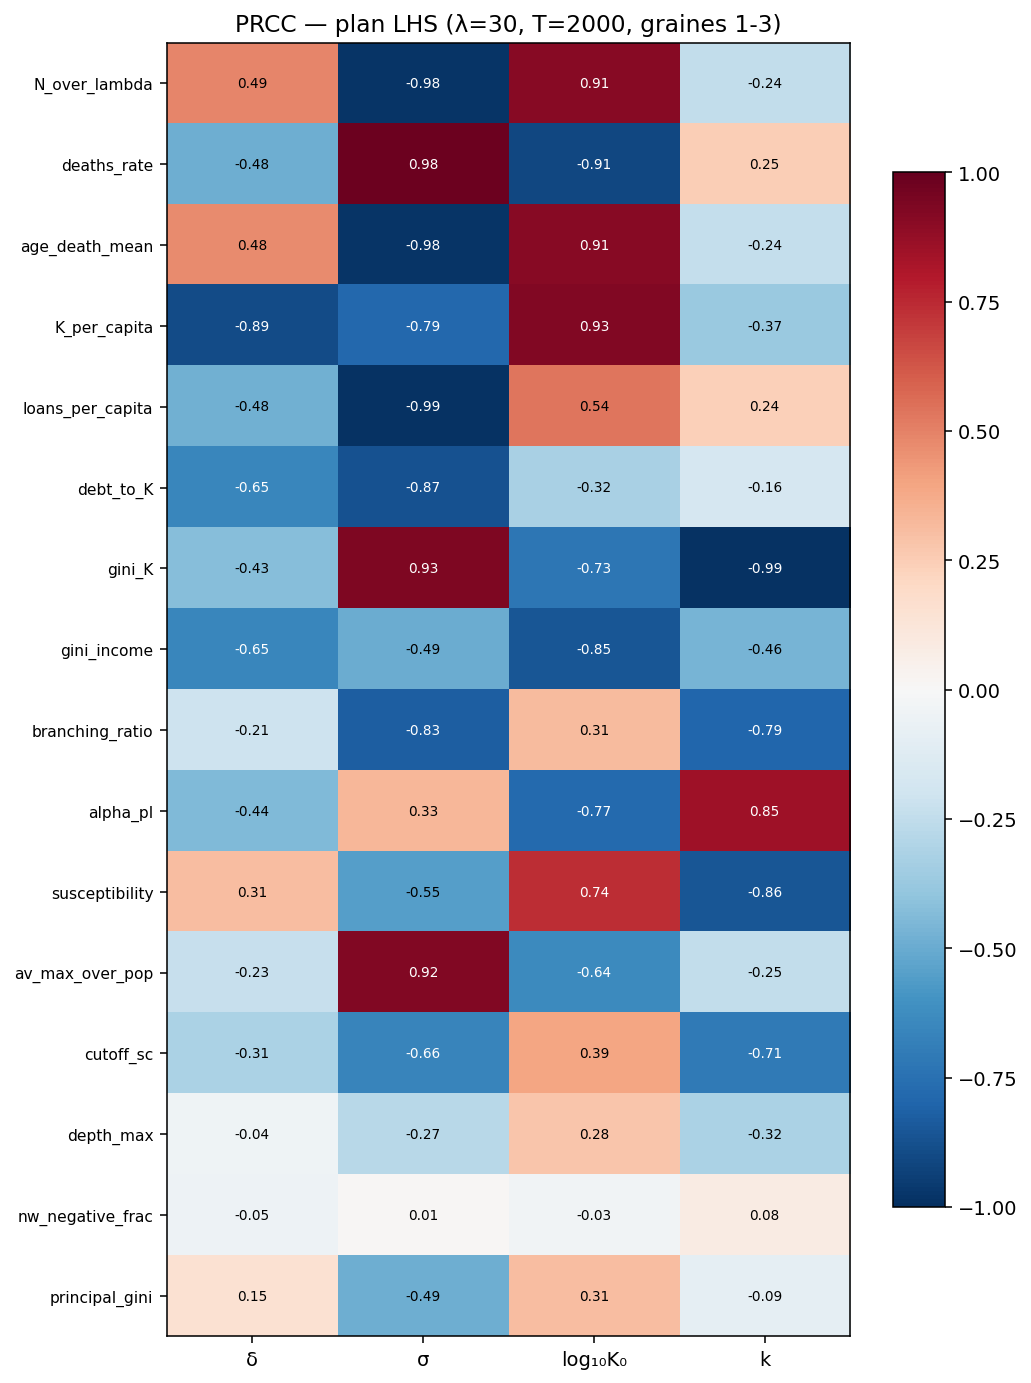
\includegraphics[width=0.72\textwidth]{lhs_prcc.png}
\caption{Corrélations de rang partielles (PRCC) sur le plan LHS
($\lambda=30$, $T=2000$, graines 1--3, 192 runs) : effet de chaque
paramètre, les autres étant tenus fixes. Lecture par colonne :
$\sigma$ domine la démographie et l'exposition ; $k$ domine le Gini du
capital et la statistique des avalanches ; $K_0$ est le second levier
démographique ; $\delta$ pèse surtout sur l'échelle du capital.}
\label{fig:prcc}
\end{figure}

\subsection{$\sigma$ : le levier dominant, et une transition douce}
\label{sec:sigma}

\begin{figure}[tbh]
\centering
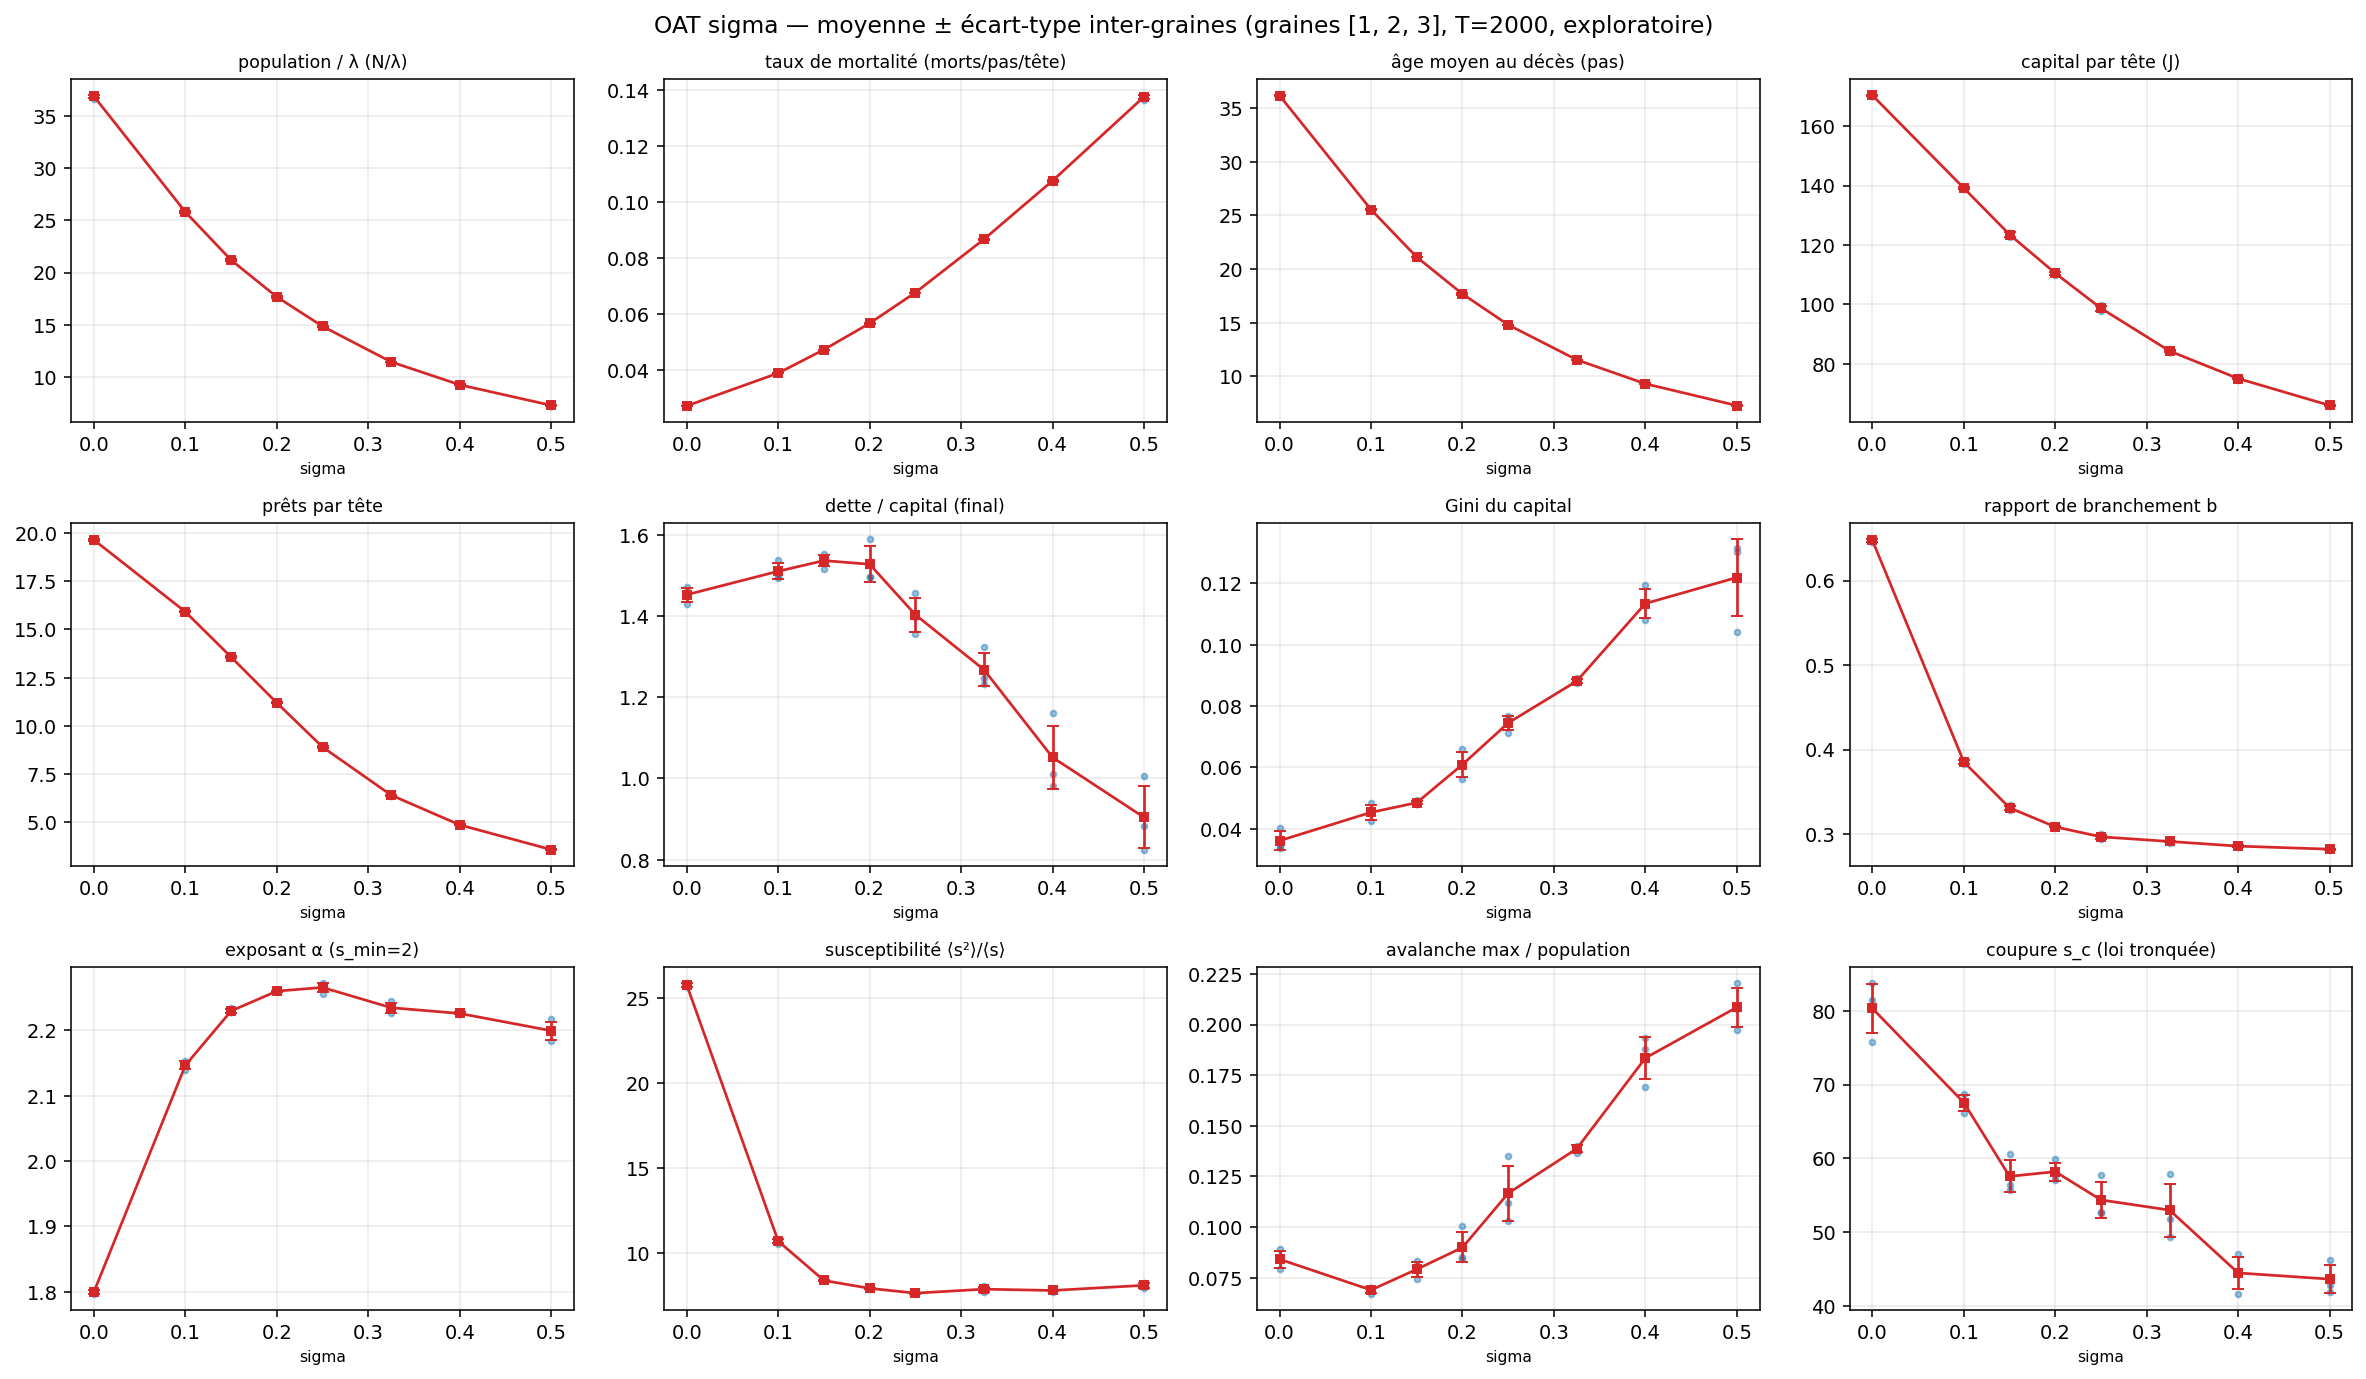
\includegraphics[width=\textwidth]{oat_sigma.png}
\caption{Courbes OAT le long de $\sigma$ (12 métriques ; points bleus :
graines ; carrés : moyenne $\pm$ écart-type). Toute la non-linéarité de
la propagation se concentre dans $\sigma\in[0,0{,}2]$ ; la dette/capital
est non monotone (maximum vers $\sigma\simeq0{,}15$--$0{,}2$).}
\label{fig:oat-sigma}
\end{figure}

Faits confirmés (contrastes vs centre, $T=4000$) : passer de
$\sigma=0{,}25$ à $0{,}10$ ajoute $+10{,}96\pm0{,}16$ pas de durée de
vie ($N/\lambda$), $+0{,}086\pm0{,}003$ de rapport de branchement et
$+0{,}149\pm0{,}084$ de dette/capital ; passer à $\sigma=0{,}50$
retire $7{,}49\pm0{,}05$ pas, $0{,}48\pm0{,}13$ de dette/capital, et
ajoute $+0{,}065\pm0{,}028$ de Gini. La figure~\ref{fig:oat-sigma}
montre la structure : mortalité convexe croissante, ralentissement des
courbes au-delà de $\sigma\simeq0{,}2$, et \emph{crête d'exposition} —
la dette rapportée au capital culmine ($\simeq1{,}53$) là où les vies
sont assez longues pour accumuler du carnet mais les écarts de capital
déjà assez grands pour motiver de gros prêts.

La zone $\sigma\in[0,0{,}2]$ est une \emph{transition douce mais
rapide} entre deux comportements de cascade : au contrôle $\sigma=0$
(confirmé sur 5 graines), $b=0{,}647\pm0{,}001$ et
$\hat\alpha=1{,}801\pm0{,}007$ — cascades très propagatives dans une
population homogène structurée par l'âge ($N/\lambda=37{,}0$, Gini
$0{,}035$) — tandis que pour $\sigma\gtrsim0{,}2$, $b$ s'épingle sur un
plateau $0{,}28$--$0{,}31$ et $\hat\alpha$ sur $2{,}2$--$2{,}3$,
indépendamment de $\sigma$. Fait notable : le régime sans choc reste
mortel et stationnaire — l'hétérogénéité d'âge suffit à alimenter
défauts, insolvabilités et cascades. Aucune discontinuité n'a été
détectée le long de cette transition (courbes continûment déformées,
figures~\ref{fig:cut-k} et \ref{fig:cut-delta}).

\subsection{$k$ : l'égalisateur, et le réglage fin des cascades}
\label{sec:k}

La démographie est quasi insensible à $k$ ($N/\lambda$ :
$+0{,}69\pm0{,}06$ à $k=2$, $-0{,}27\pm0{,}07$ à $k=10$, contre une
gamme de $\pm11$ pour $\sigma$), mais $k$ est le premier déterminant des
inégalités et de la statistique fine : contrastes confirmés
$\Delta\mathrm{Gini}(K)=+0{,}065\pm0{,}006$ ($k=2$) et
$-0{,}064\pm0{,}005$ ($k=10$) ; $\Delta b=-0{,}060\pm0{,}003$ et
$\Delta\hat\alpha=+0{,}178\pm0{,}012$ à $k=10$. Interprétation
(hypothèse mécanique) : un échantillon plus grand sélectionne des
paires riche--pauvre plus contrastées et tire les deux parties vers la
cible commune $K^\ast=\sqrt{K_\ell K_b}$ ; le marché devient un
égalisateur de capital (Gini $0{,}010$ à $k=10$), ce qui fragmente les
expositions, raccourcit les cascades ($b$ plus faible) et raidit la
queue ($\hat\alpha$ plus grand).

\subsection{$K_0$ : protection log-linéaire des jeunes}

$N/\lambda$ croît quasi linéairement en $\log K_0$ ($10{,}7$ à
$K_0=5$, $19{,}9$ à $K_0=100$ ; contrastes confirmés
$-4{,}17\pm0{,}04$ et $+4{,}97\pm0{,}07$). Le rapport de branchement
est remarquablement insensible ($\pm0{,}012$ au plus), l'exposant
$\hat\alpha$ décroît modérément avec $K_0$ ($+0{,}072$ à $K_0=5$,
$-0{,}106$ à $K_0=100$). $K_0$ est donc un levier démographique quasi
pur : il fixe la vulnérabilité de l'enfance des entités sans
restructurer la propagation.

\subsection{$\delta$ : une échelle du capital, avec une réserve}
\label{sec:delta}

$\delta$ contrôle fortement l'échelle du capital individuel
($K$ par tête : $159$~J à $\delta=0{,}02$, $51$~J à $0{,}10$ ;
PRCC $-0{,}89$) et l'exposition (dette/capital $-0{,}23\pm0{,}10$ à
$\delta=0{,}10$), mais faiblement le reste : les contrastes confirmés
sur $b$ et $\hat\alpha$ restent $\le0{,}006$ et $\le0{,}05$ en valeur
absolue. Effet contre-intuitif confirmé : la durée de vie
\emph{augmente} avec la dépréciation ($\Delta N/\lambda=
-1{,}32\pm0{,}06$ à $\delta=0{,}02$, $+2{,}18\pm0{,}07$ à
$\delta=0{,}10$). Hypothèse d'interprétation, à trancher par l'étude
analytique de M5 : $\delta$ élevé rapproche les capitaux du point fixe
individuel $K^\ast=(1/\delta)^2$ plus bas, augmente le produit marginal
$1/(2\sqrt K)$ et le rendement de la production concave relativement au
stock, ce qui raccourcit la convalescence des jeunes emprunteuses ; la
dette nominale héritée pèse aussi moins longtemps puisque le carnet est
plus petit devant les flux.

\emph{Réserve importante} (coupe $\sigma\times\delta$,
figure~\ref{fig:cut-delta}) : cette lecture « échelle » vaut pour
$\sigma\ge0{,}2$, où les courbes de propagation ($b$, susceptibilité,
Gini) s'effondrent sur une courbe maîtresse indépendante de $\delta$.
Dans le régime faiblement bruité, $\delta$ module la propagation
($b$ à $\sigma=0{,}05$ : $0{,}50$ pour $\delta\le0{,}05$ contre
$0{,}43$ pour $\delta=0{,}10$ ; contraste confirmé de la cellule
d'interaction $(\sigma{=}0{,}05,\delta{=}0{,}10)$ :
$\Delta b=+0{,}134\pm0{,}003$ contre $+0{,}217\pm0{,}002$ pour
$(\sigma{=}0{,}05,k{=}2)$).

\subsection{$\lambda$ : un pur axe de taille finie}
\label{sec:lambda}

Les grandeurs intensives — $N/\lambda$, âge au décès, capital par
tête, Gini, dette/capital, $b$ — sont stables à $\pm2\,\%$ de
$\lambda=10$ à $100$ (et l'intensivité de $N/\lambda$ tient, à
$\pm3\,\%$, jusqu'à $\lambda=2$ ; à $\lambda=1$, la seule graine
survivante donne encore $15{,}4$). Les micro-écarts démographiques suggérés par
l'exploration ($\mp1$--$2\,\%$) ne se sont \emph{pas} reproduits en
confirmation (section~\ref{sec:negatifs}) : nous concluons à
l'intensivité pure. Ce qui dépend de $\lambda$ est la physique de
taille finie des avalanches (section~\ref{sec:avalanches}).

\section{Interactions}
\label{sec:interactions}

\begin{figure}[tbh]
\centering
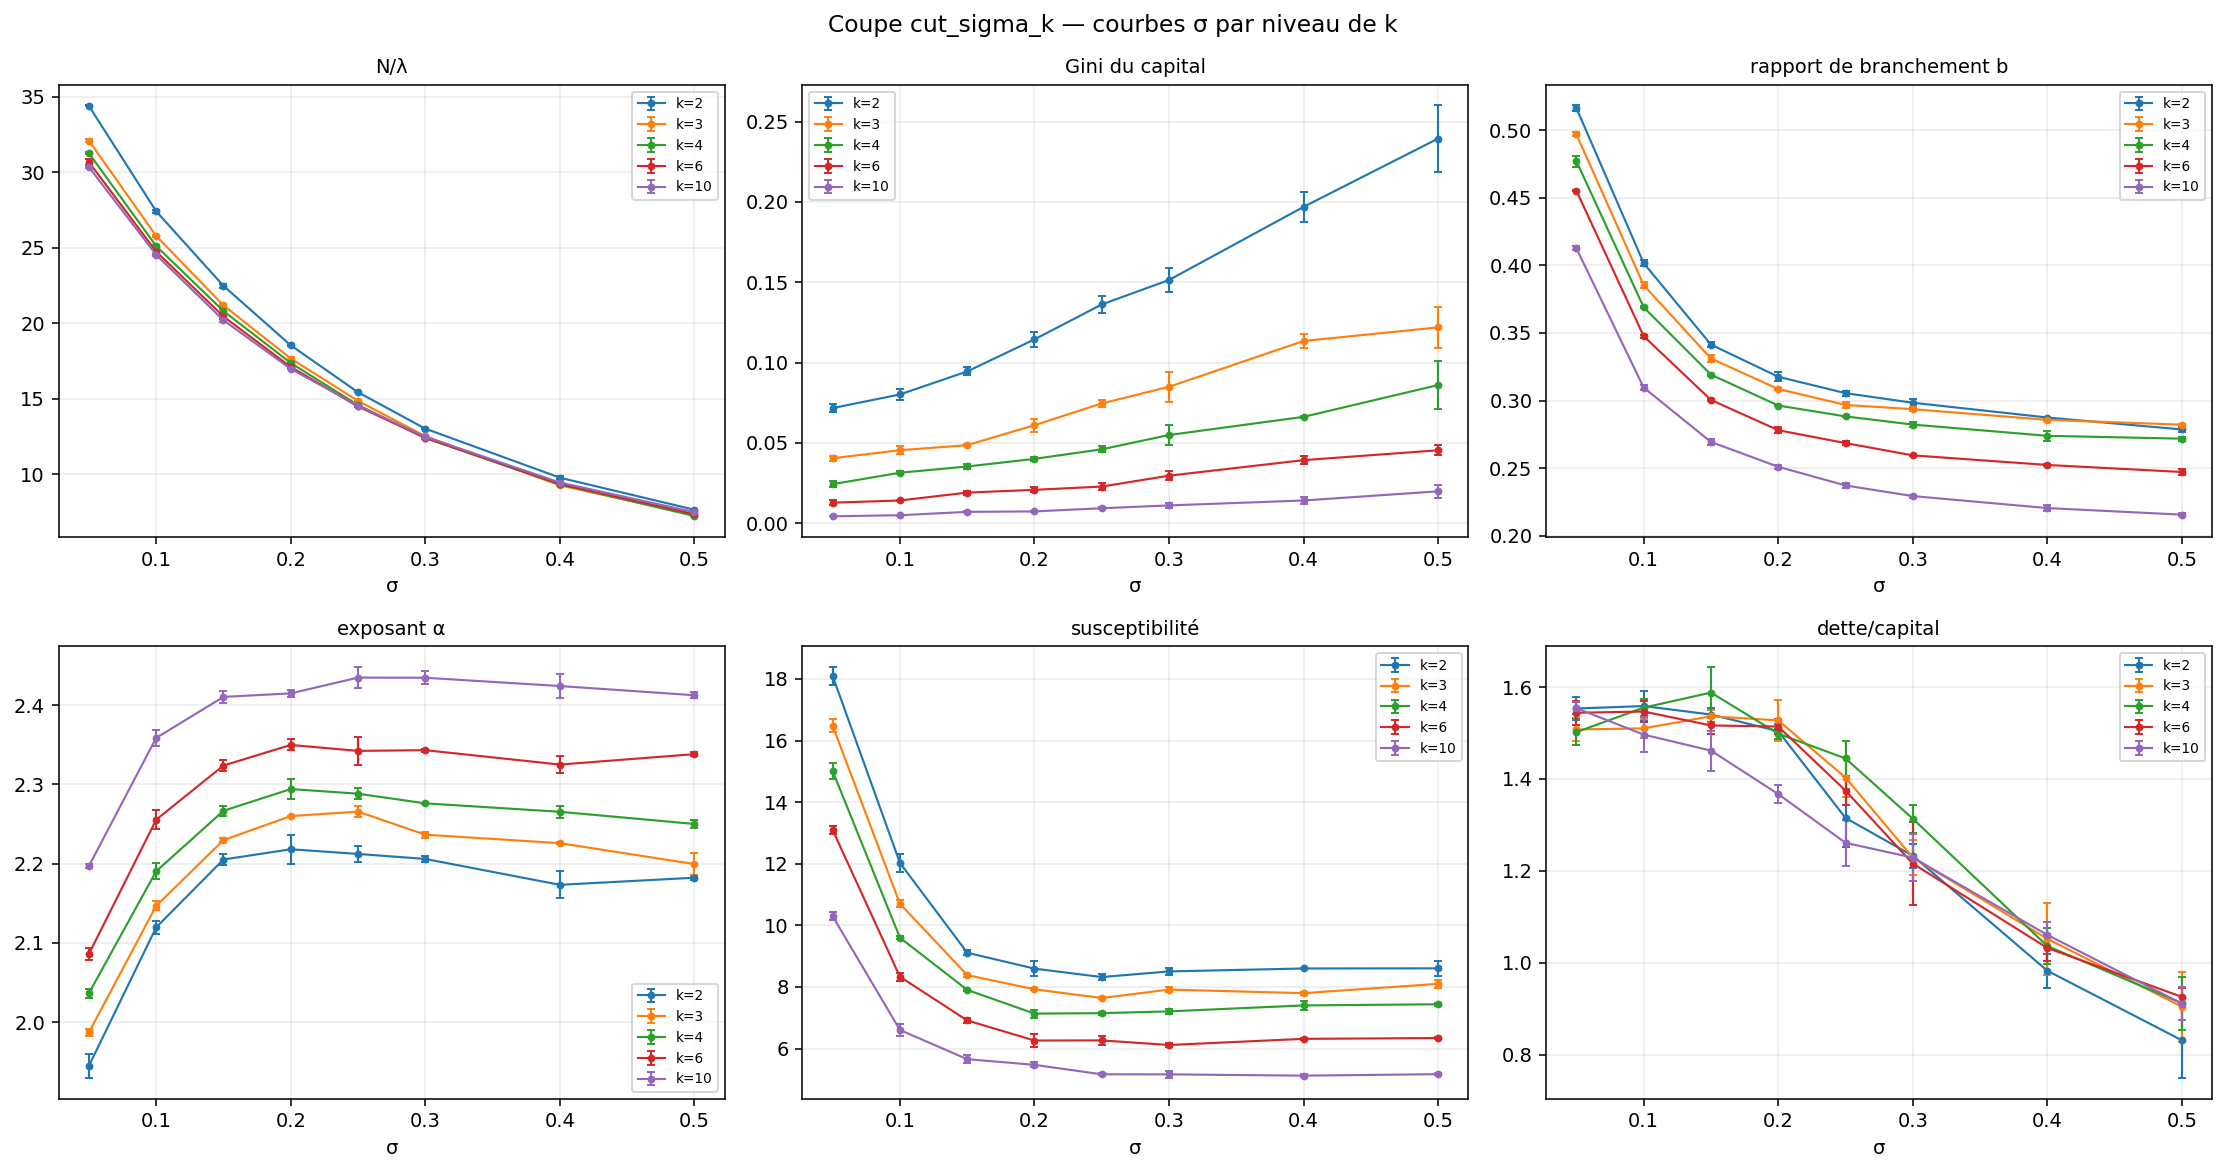
\includegraphics[width=\textwidth]{cut_sigma_k_lines.png}
\caption{Coupe $\sigma\times k$ (moyennes $\pm$ écart-type,
graines 1--3). Pas de croisement qualitatif : la transition en
$\sigma$ n'est pas déplacée par $k$. L'interaction est quantitative :
le Gini s'évase (à $\sigma=0{,}5$ : $0{,}24$ pour $k=2$ contre
$0{,}02$ pour $k=10$), tandis que $N/\lambda$ et la dette/capital
suivent des courbes maîtresses quasi indépendantes de $k$.}
\label{fig:cut-k}
\end{figure}

\begin{figure}[tbh]
\centering
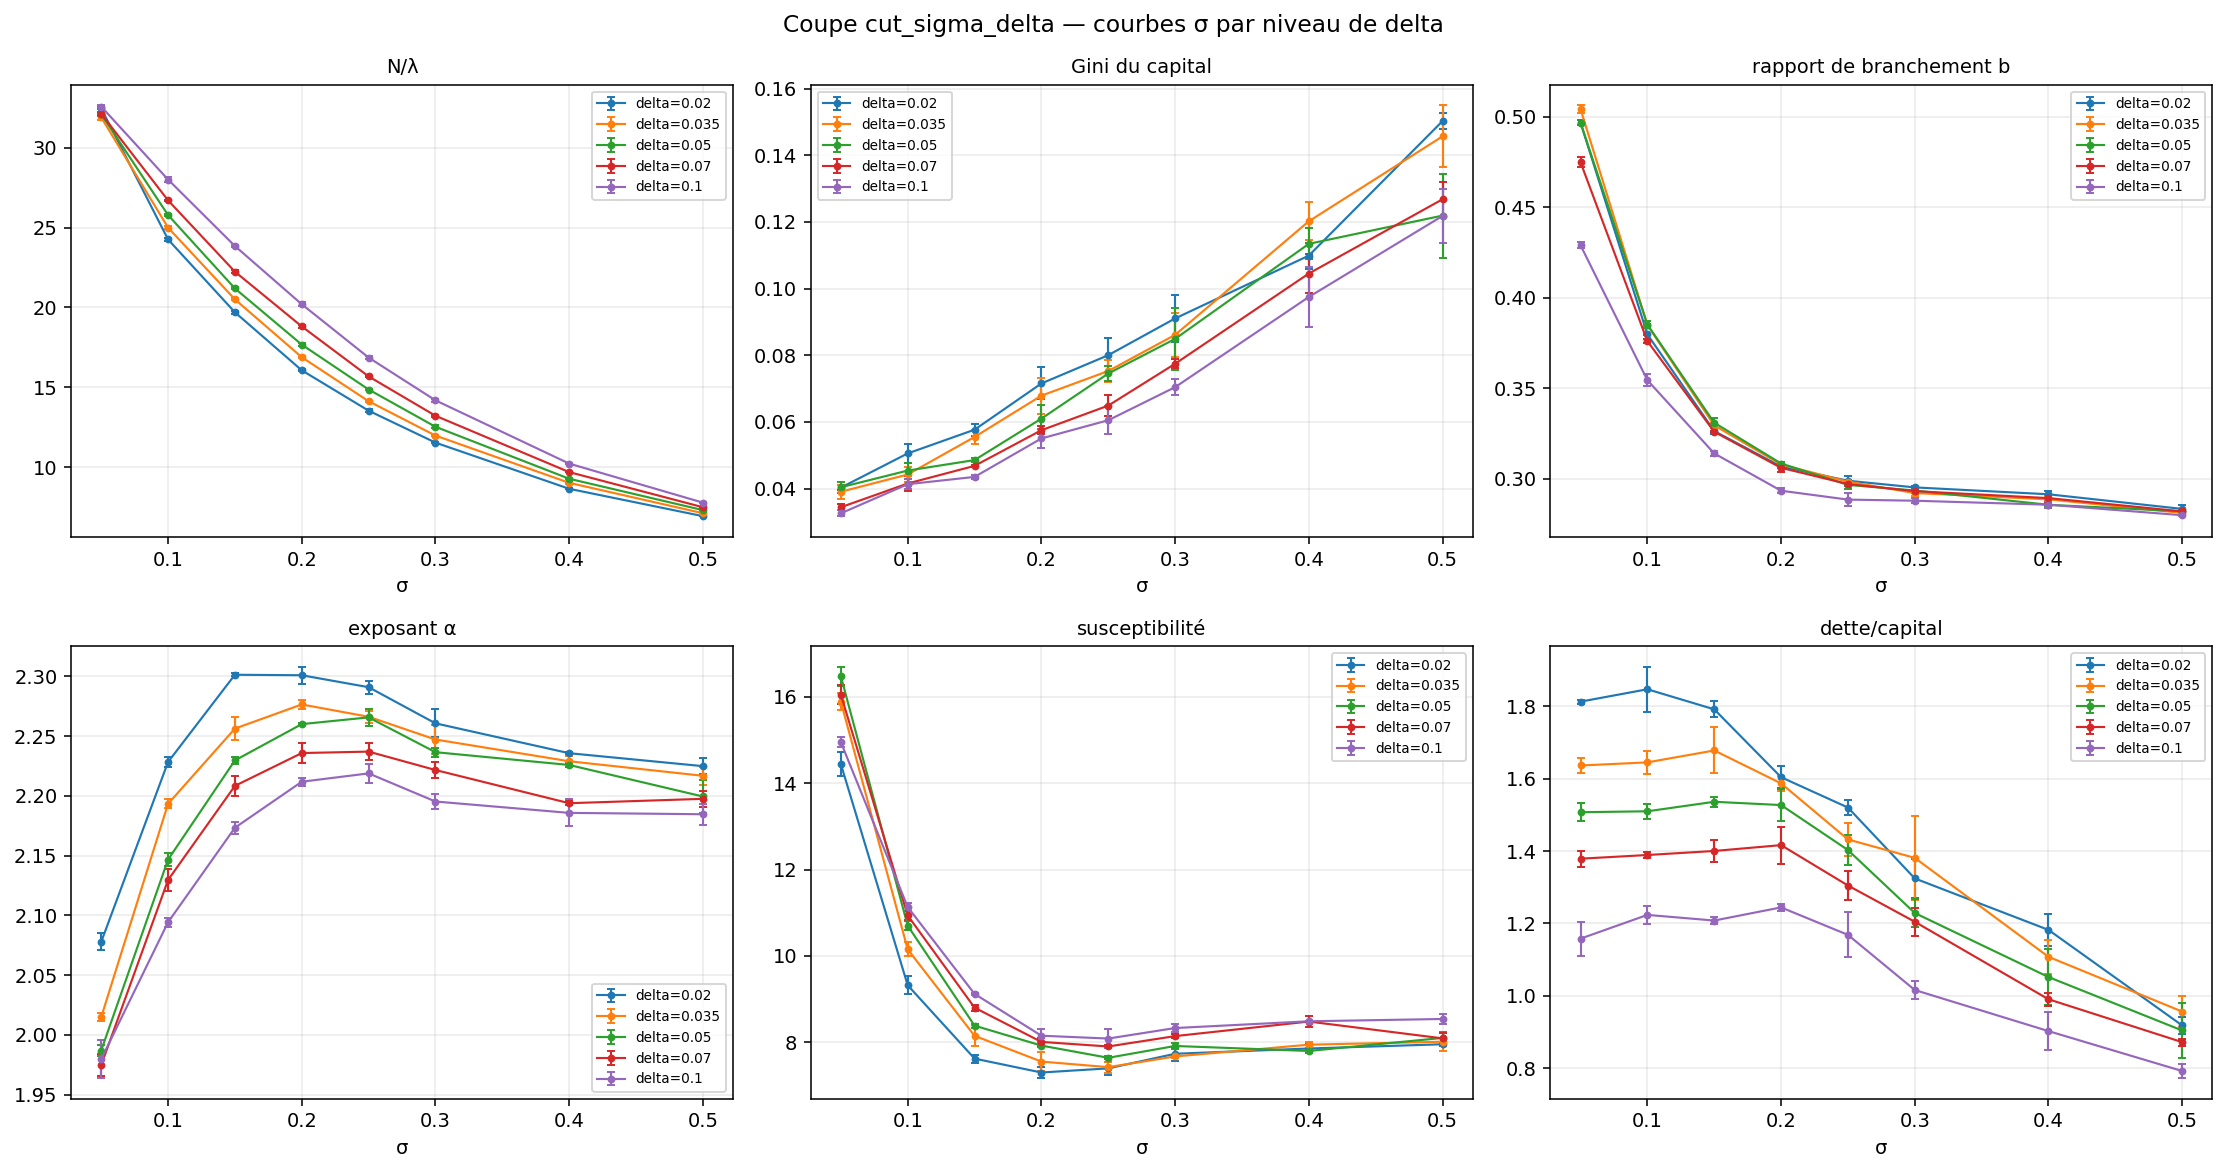
\includegraphics[width=\textwidth]{cut_sigma_delta_lines.png}
\caption{Coupe $\sigma\times\delta$. À $\sigma\ge0{,}2$, $b$,
susceptibilité et Gini s'effondrent sur une courbe commune (lecture
« $\delta$ = échelle ») ; à $\sigma<0{,}15$, $\delta$ module la
propagation. La dette/capital garde sa bosse basse-$\sigma$ à tout
$\delta$, avec un niveau d'ensemble décroissant en $\delta$.}
\label{fig:cut-delta}
\end{figure}

Les deux coupes bidimensionnelles ciblées après le screening
(figures~\ref{fig:cut-k} et \ref{fig:cut-delta}) écartent tout
croisement qualitatif : aucune interaction ne déplace la transition en
$\sigma$, n'inverse un signe d'effet ni ne crée de nouveau régime.
Deux interactions quantitatives sont établies et confirmées :

\begin{enumerate}
\item \textbf{Évasement des inégalités ($\sigma\times k$).} La
  volatilité n'engendre d'inégalité durable que si le marché égalise
  mal : le Gini croît fortement avec $\sigma$ à $k=2$ et reste presque
  nul à $k=10$. Cellule confirmatoire $(\sigma{=}0{,}5,k{=}2)$ :
  $\Delta\mathrm{Gini}=+0{,}169\pm0{,}042$ contre $+0{,}065$ pour
  $\sigma=0{,}5$ seul et $+0{,}065$ pour $k=2$ seul — surenchère
  claire au-delà de l'additivité.
\item \textbf{Module basse-volatilité de $\delta$
  ($\sigma\times\delta$).} Décrit en section~\ref{sec:delta} : l'effet
  de $\delta$ sur la propagation est confiné au régime corrélé
  $\sigma<0{,}15$.
\end{enumerate}

\section{Avalanches : loi tronquée, coupure de taille finie, plateau de
branchement}
\label{sec:avalanches}

\begin{table}[tbh]
\centering
\small
\begin{tabular}{@{}lrrrrrr@{}}
\toprule
Cellule & $\hat\alpha$ (pur) & $b$ & Vuong $z$ & $\hat s_c$ & $s_{\max}$ \\
\midrule
$\lambda=10$ & $2{,}312\pm0{,}013$ & $0{,}292\pm0{,}002$ & $-9{,}1$ (5/5 nég.) & $10{,}0$ & $29$ \\
centre $\lambda=30$ & $2{,}248\pm0{,}003$ & $0{,}297\pm0{,}002$ & $-5{,}7$ (5/5 nég.) & $51{,}6$ & $54$ \\
$\lambda=100$ & $2{,}318\pm0{,}003$ & $0{,}300\pm0{,}001$ & $+21{,}0$ (5/5 pos.) & n.i. & $110$ \\
$\sigma=0$ & $1{,}801\pm0{,}007$ & $0{,}647\pm0{,}001$ & $-12{,}9$ & $80{,}7$ & $100$ \\
$\sigma=0{,}10$ & $2{,}157\pm0{,}005$ & $0{,}383\pm0{,}001$ & $-6{,}8$ & $69{,}0$ & $60$ \\
$\sigma=0{,}50$ & $2{,}207\pm0{,}008$ & $0{,}282\pm0{,}002$ & $-7{,}1$ & $43{,}7$ & $47$ \\
$k=2$ & $2{,}217\pm0{,}008$ & $0{,}305\pm0{,}003$ & $-5{,}8$ & $57{,}6$ & $52$ \\
$k=10$ & $2{,}426\pm0{,}012$ & $0{,}237\pm0{,}001$ & $-5{,}1$ & $37{,}9$ & $45$ \\
$K_0=5$ / $K_0=100$ & $2{,}32$ / $2{,}14$ & $0{,}295$ / $0{,}309$ & nég. & $47$ / $55$ & $50$ / $57$ \\
$\delta=0{,}02$ / $0{,}10$ & $2{,}28$ / $2{,}20$ & $0{,}301$ / $0{,}291$ & nég. & $56$ / $51$ & $51$ / $56$ \\
\bottomrule
\end{tabular}
\caption{Lois de tailles d'avalanches par cellule confirmatoire
(5 graines ; ajustements par graine puis agrégés ; fenêtre
$[1000,4000]$, $s\ge2$, 4\,300--33\,000 événements par graine selon la
cellule — 11\,000 au centre). $\hat\alpha$ : MLE discrète de la loi pure ; $b$ : rapport de
branchement ; Vuong $z<0$ : la log-normale discrète bat la loi pure,
$z>0$ l'inverse ; $\hat s_c$ : coupure de la loi tronquée
(« n.i. » : non identifiable, coupure au-delà de la portée
observable) ; $s_{\max}$ : plus grande avalanche (moyenne). Le rapport
de vraisemblance de la loi tronquée contre la loi pure est significatif
partout ($p<10^{-6}$ pour chaque graine).}
\label{tab:lois}
\end{table}

\begin{figure}[tbh]
\centering
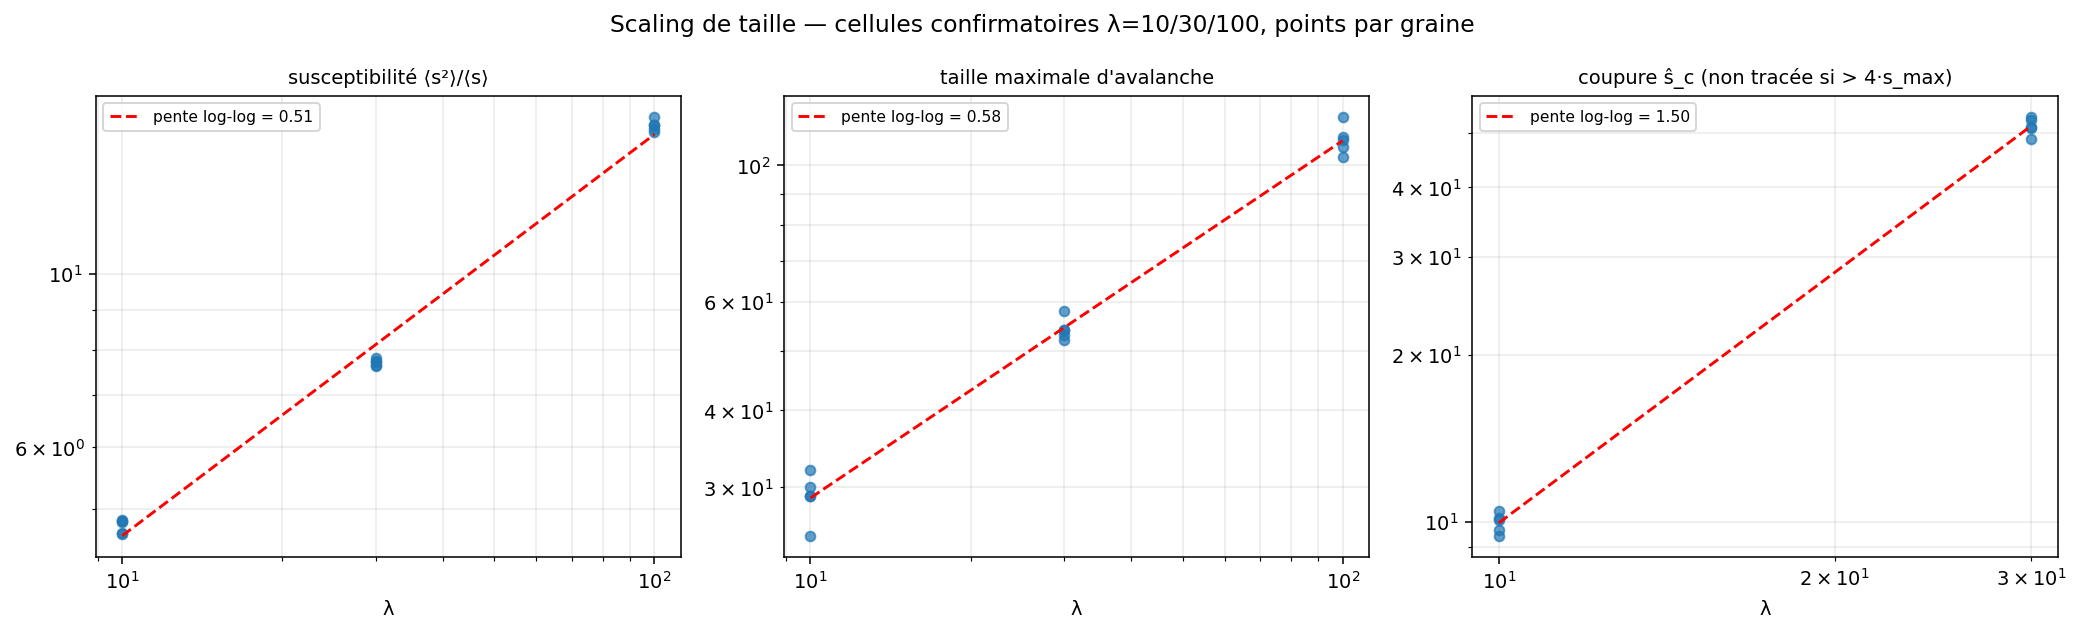
\includegraphics[width=\textwidth]{confirm_scaling.png}
\caption{Scaling de taille finie ($\lambda=10/30/100$, un point par
graine confirmatoire). Susceptibilité
$\langle s^2\rangle/\langle s\rangle\propto\lambda^{0{,}51}$ ; taille
maximale $\propto\lambda^{0{,}58}$ ; coupure ajustée
$\hat s_c\propto\lambda^{1{,}5}$ entre $\lambda=10$ et $30$ (à
$\lambda=100$ la coupure sort de la fenêtre observable et n'est pas
tracée).}
\label{fig:scaling}
\end{figure}

La table~\ref{tab:lois} et la figure~\ref{fig:scaling} rassemblent la
statistique des cascades. Trois conclusions robustes :

\begin{enumerate}
\item \textbf{La loi de puissance tronquée est la description
  cohérente à toutes les tailles.} À chaque graine de chaque cellule,
  la loi tronquée bat significativement la loi pure (LRT,
  $p<10^{-6}$). Le test de Vuong contre la log-normale discrète est
  négatif à $\lambda\le30$ — signature d'une coupure serrée — et
  bascule franchement en faveur de la loi de puissance à $\lambda=100$
  ($z=+21{,}0\pm0{,}9$, 5/5 graines), où la coupure ajustée sort de la
  fenêtre observable. La coupure croît vite avec la taille du système
  ($\hat s_c$ : $10{,}0\to51{,}6$ pour $\lambda$ : $10\to30$, pente
  log-log $1{,}5$), le maximum comme $\lambda^{0{,}58}$ et la
  susceptibilité comme $\lambda^{0{,}51}$.
\item \textbf{L'exposant asymptotique est
  $\alpha\simeq2{,}31$.} L'exposant de la loi \emph{pure} paraît non
  monotone en $\lambda$ ($2{,}312/2{,}248/2{,}318$) ; celui de la loi
  \emph{tronquée} est monotone ($1{,}584\pm0{,}035$,
  $2{,}041\pm0{,}009$, $2{,}313\pm0{,}003$) et rejoint la loi pure à
  $\lambda=100$. La non-monotonie du fit pur est donc un artefact de
  taille finie (compensation de la coupure par un raidissement), et la
  meilleure estimation de l'exposant de grand système est
  $\alpha=2{,}31$--$2{,}32$.
\item \textbf{Le plateau $b\simeq0{,}30$ est institutionnel.} Hors
  transition basse-$\sigma$, le rapport de branchement reste dans
  $[0{,}28;0{,}31]$ pour toutes les valeurs de $\sigma\ge0{,}2$,
  $\delta$, $K_0$ et $\lambda$ ; seuls $k$ (jusqu'à $0{,}237$ à
  $k=10$) et le régime corrélé ($0{,}38$ à $\sigma=0{,}10$, $0{,}51$ à
  $(\sigma{=}0{,}05,k{=}2)$, $0{,}647$ à $\sigma=0$) l'en délogent.
  Ceci prolonge le résultat institutionnel de M4 (un round de marché
  par tête épingle $b$) en précisant ses deux seules conditions de
  validité : bruit suffisant et échantillon de marché petit.
\end{enumerate}

\section{Distributions individuelles et renouvellement}
\label{sec:distributions}

\begin{figure}[tbh]
\centering
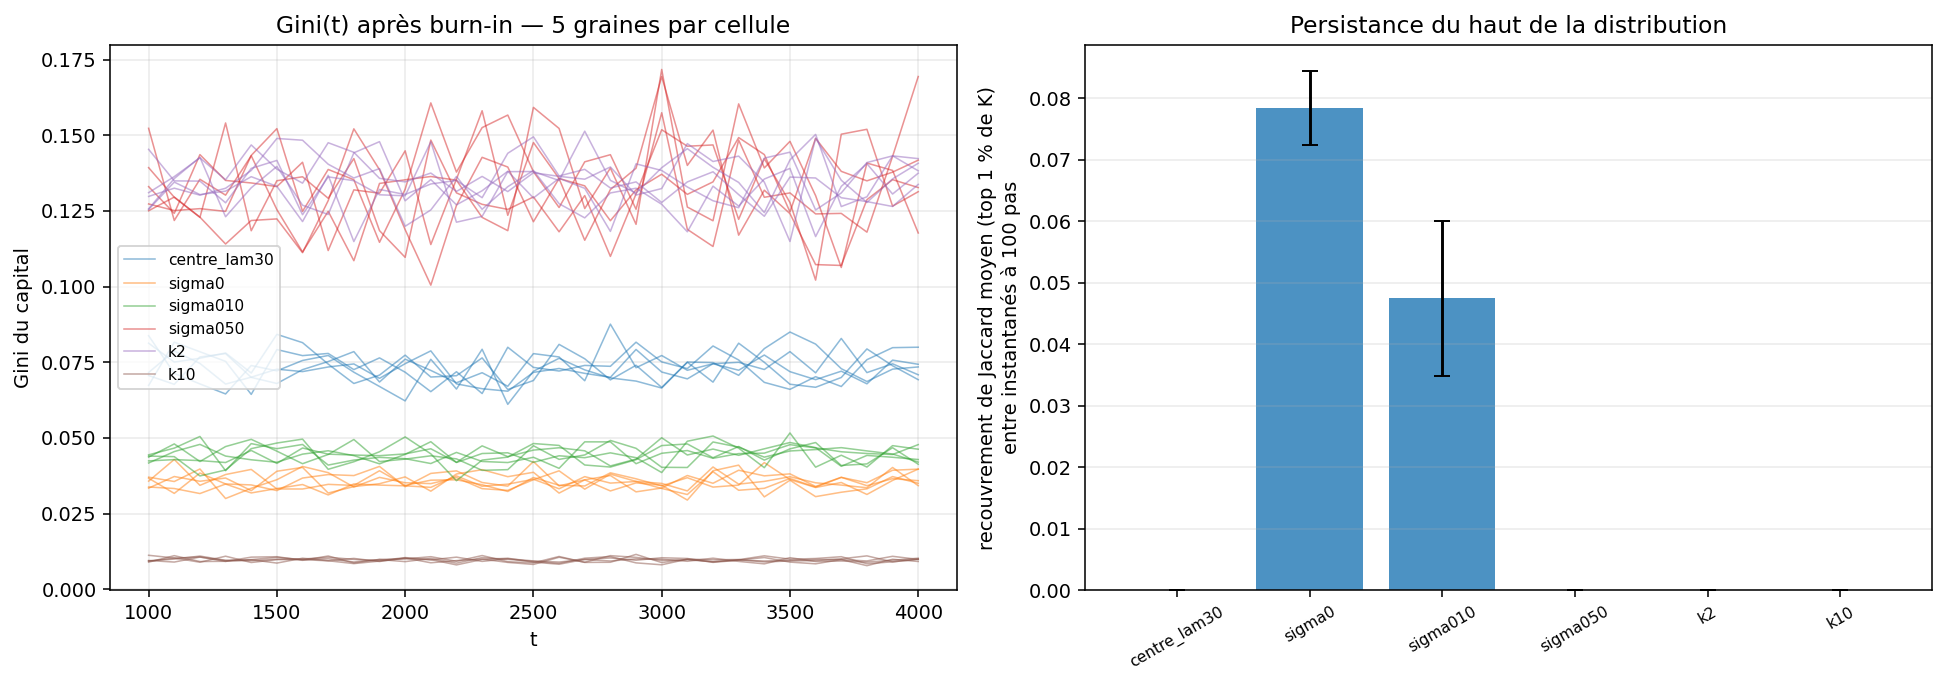
\includegraphics[width=\textwidth]{confirm_gini_renewal.png}
\caption{Gauche : trajectoires du Gini du capital après burn-in
(5 graines par cellule, instantanés tous les 100 pas) — stationnaires
et bien séparées. Droite : persistance du top 1\,\% du capital entre
instantanés espacés de 100 pas (recouvrement de Jaccard moyen).}
\label{fig:gini}
\end{figure}

\begin{figure}[tbh]
\centering
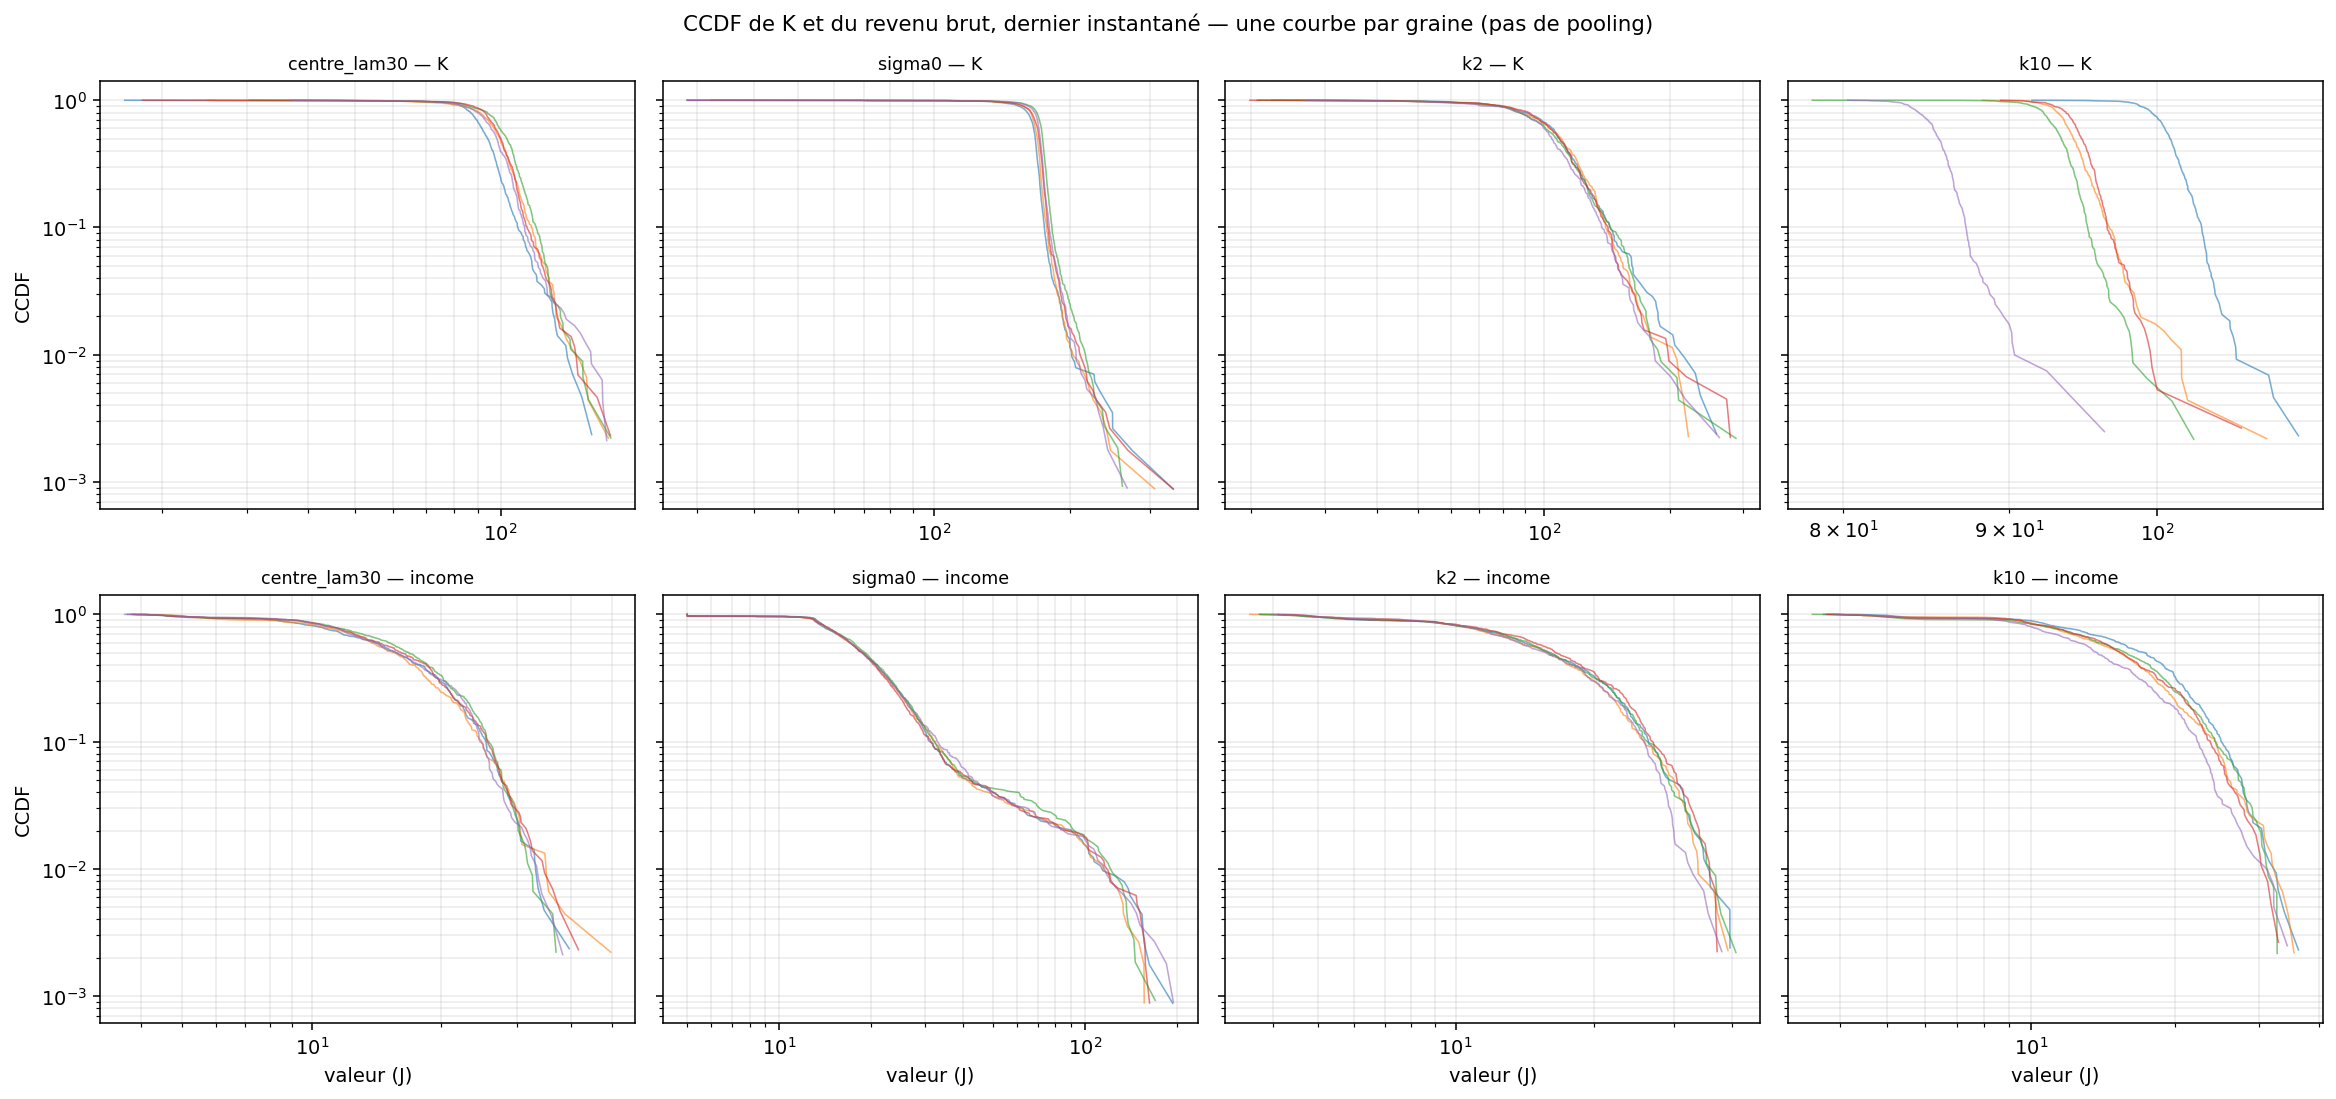
\includegraphics[width=\textwidth]{confirm_ccdf.png}
\caption{Fonctions de survie (CCDF) du capital et du revenu brut au
dernier instantané, une courbe par graine (jamais de fusion
inter-graines). Le capital est distribué de façon compacte (l'entité
meurt avant d'accumuler) ; le revenu porte une queue plus étalée,
d'où son Gini plus élevé. À $k=10$ le support du capital devient très
étroit (homogénéisation par le marché) ; à $\sigma=0$ la CCDF du revenu
présente un épaulement lié aux revenus d'intérêts des prêteuses âgées.}
\label{fig:ccdf}
\end{figure}

Les figures~\ref{fig:gini} et \ref{fig:ccdf} résument le volet
distributionnel. Faits : le Gini du capital est stationnaire dans
toutes les cellules et hiérarchisé exactement comme la théorie des
rôles le prédit ($0{,}010$ à $k=10$ ; $0{,}035$ à $\sigma=0$ ;
$0{,}074$ au centre ; $0{,}13$--$0{,}14$ à $\sigma=0{,}5$ et à
$k=2$). Le haut de la distribution se renouvelle intégralement à
l'échelle de 100 pas (recouvrement de Jaccard nul), sauf faible
persistance dans les régimes à vies longues ($0{,}078\pm0{,}006$ à
$\sigma=0$ ; $0{,}047\pm0{,}013$ à $\sigma=0{,}10$) : la persistance
au sommet est bornée par la durée de vie individuelle — le modèle n'a
ni héritage ni transmission, donc pas de dynasties. Le contrôle par
l'âge réserve une surprise : la corrélation de Spearman âge--capital au
dernier instantané est \emph{modérée partout} ($0{,}15$--$0{,}29$) et
gouvernée par $k$ ($0{,}29\pm0{,}06$ à $k=2$ ; $0{,}01\pm0{,}03$ à
$k=10$) bien plus que par $\sigma$ ($0{,}23$ à $\sigma=0$, $0{,}20$ à
$\sigma=0{,}5$) : même sans choc, le marché du crédit découple le
capital de l'âge en tirant prêteuses et emprunteuses vers des cibles
communes — l'interprétation « cohortes » des distributions ne doit donc
pas être poussée au-delà de ce que cette corrélation autorise. Enfin,
aucune entité survivante ne porte de valeur nette
négative (variance nulle sur 594 runs) : c'est un invariant de la règle
de faillite, vérifié plutôt qu'une métrique.

\section{La valeur nette : inégalités de bilan, cycle de vie du crédit et
bilans de décès}
\label{sec:nw}

La valeur nette $\NW_i=K_i+C_i-D_i$ est la variable d'état de la
mortalité ($\NW<0$ déclenche la faillite) ; c'est aussi la seule
grandeur individuelle qui garde la mémoire des positions de crédit. Son
agrégat est identiquement le capital total
($\sum_i C_i=\sum_i D_i$, donc $\sum\NW=\sum K$) : toute l'information
est \emph{distributionnelle}. Cette section — extension ajoutée après
l'audit, sur les mêmes runs pré-enregistrés (aucune simulation
nouvelle ; tables \path{results/summary/nw_*.csv}) — lui est dédiée.

\begin{figure}[tbh]
\centering
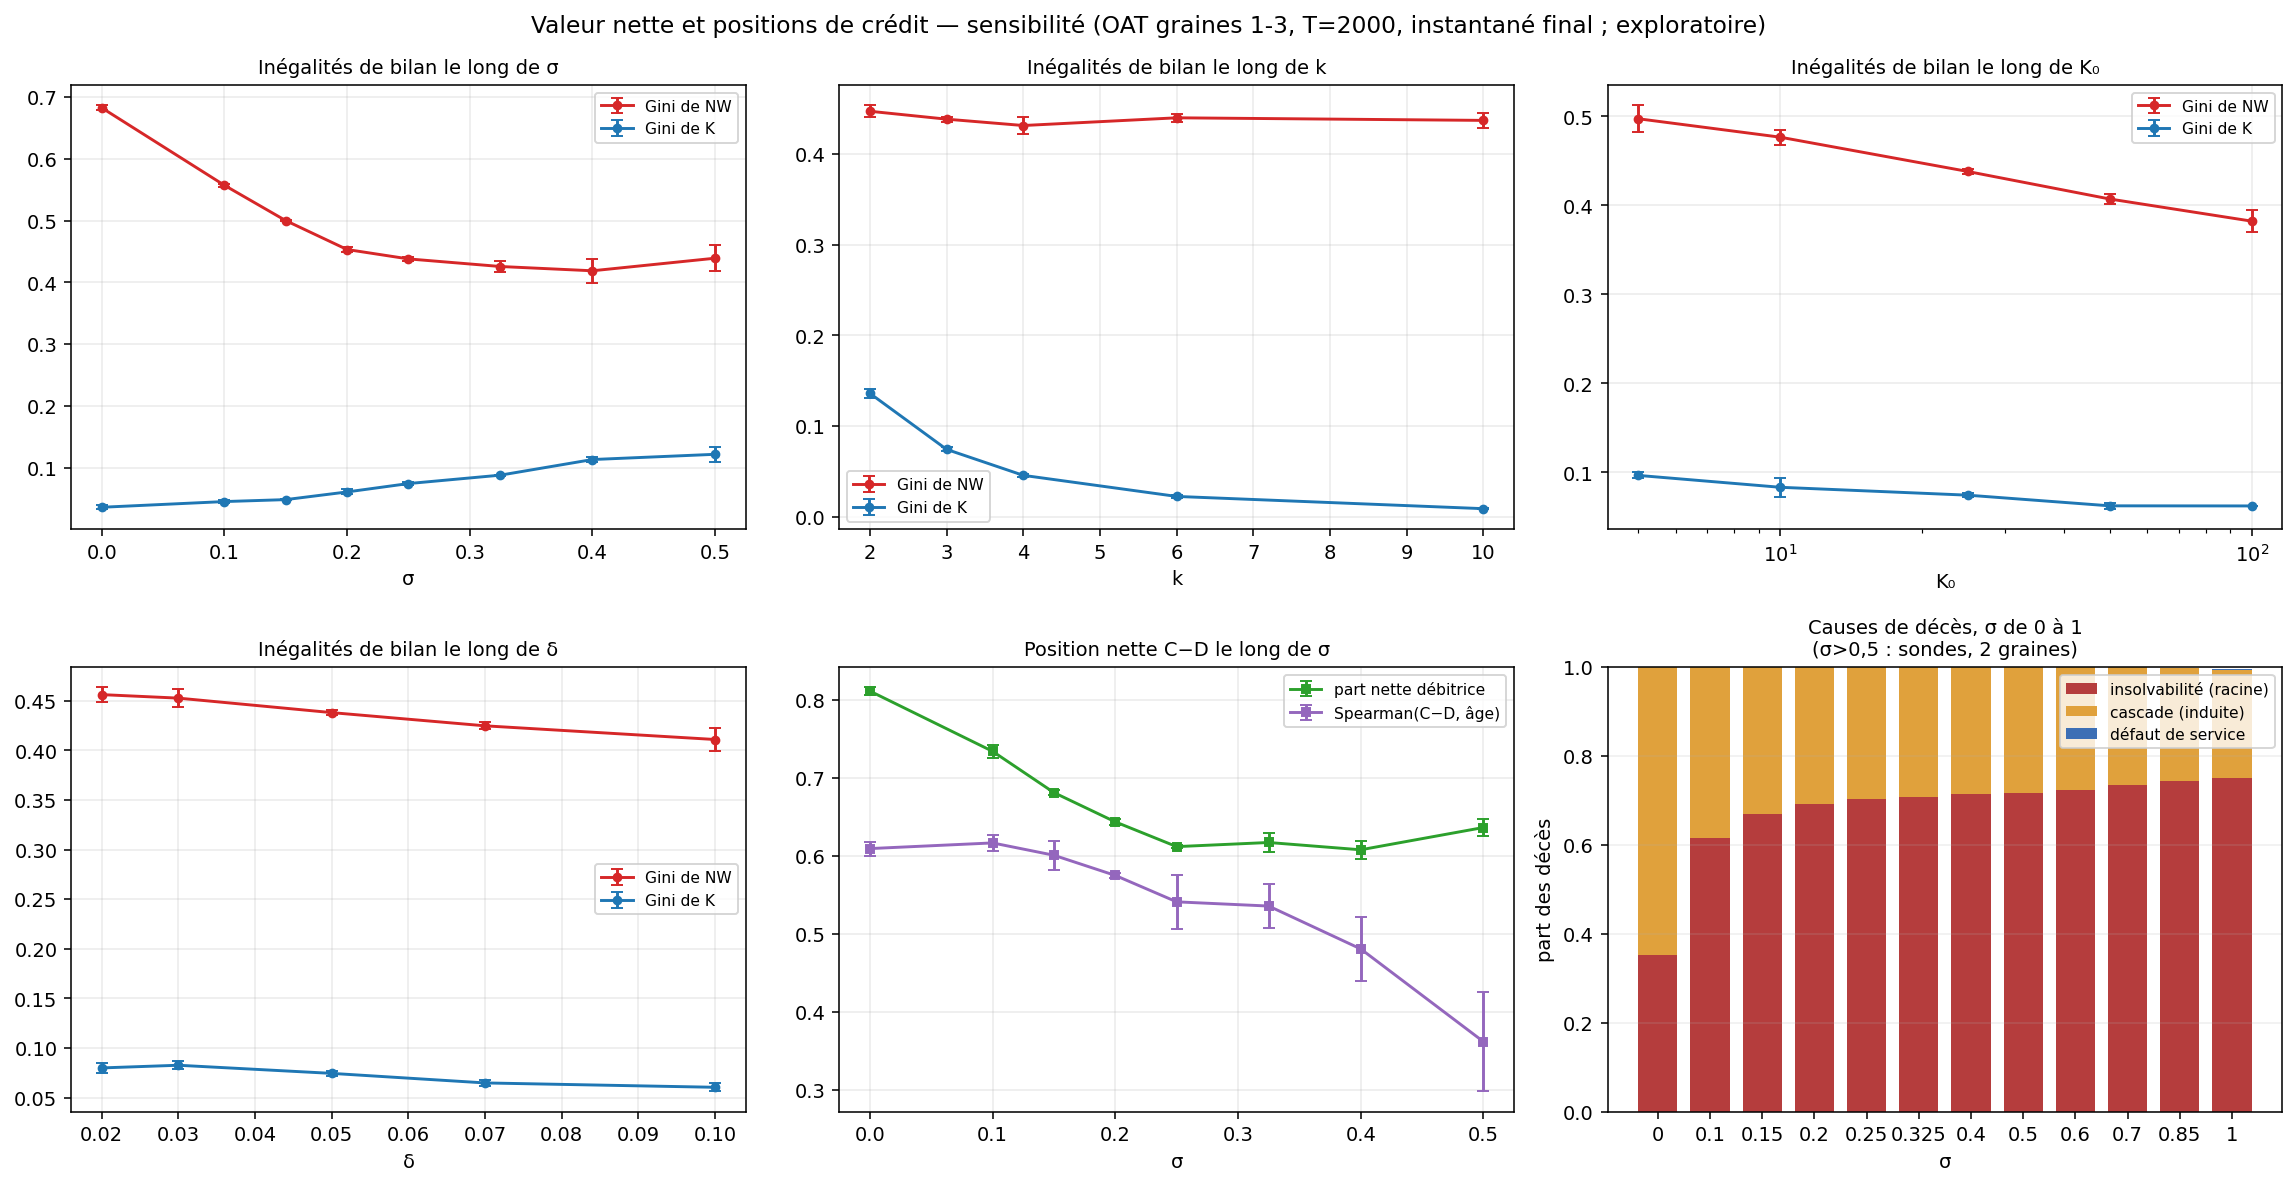
\includegraphics[width=\textwidth]{nw_sensibilite.png}
\caption{Sensibilité des bilans (OAT, graines 1--3, instantané final,
exploratoire). Haut : Gini de la valeur nette contre Gini du capital le
long de $\sigma$, $k$ et $K_0$ ; bas : le long de $\delta$ ; part
d'entités nettes débitrices et corrélation de rang entre position nette
$C-D$ et âge le long de $\sigma$ ; décomposition des causes de décès
avec $\sigma$ prolongé jusqu'à 1 par les sondes de frontière (deux
graines au-delà de $0{,}5$).}
\label{fig:nw-sens}
\end{figure}

\begin{figure}[tbh]
\centering
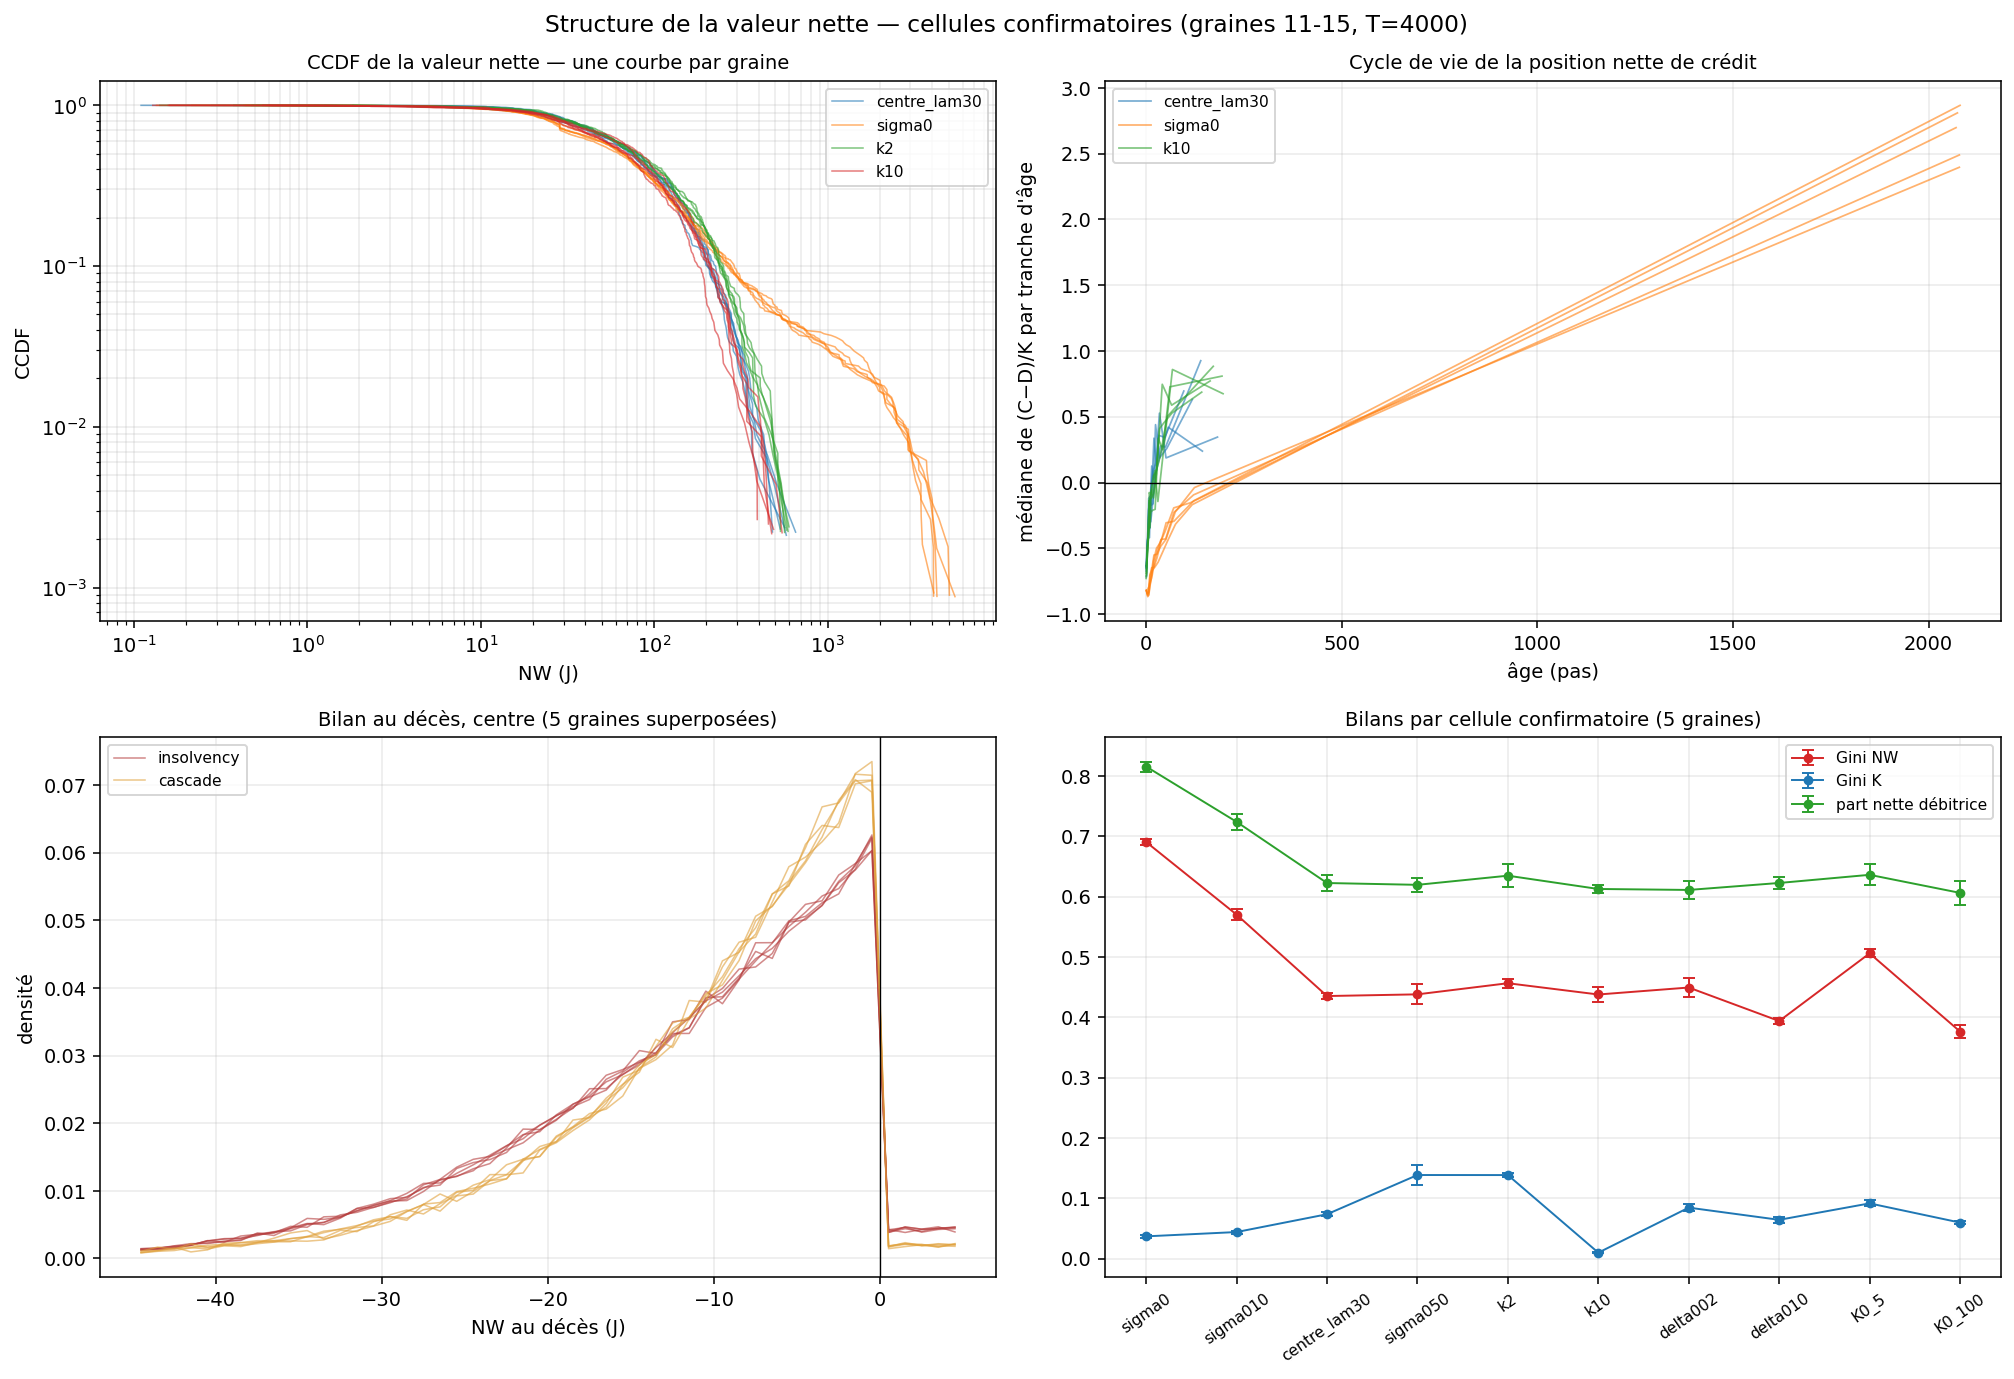
\includegraphics[width=\textwidth]{nw_structure.png}
\caption{Structure de la valeur nette (cellules confirmatoires, graines
11--15, $T=4000$). (a) CCDF de $\NW$, une courbe par graine : la
cellule $\sigma=0$ développe une queue de créancières un ordre de
grandeur au-delà des autres. (b) Médiane de $(C-D)/K$ par tranche
d'âge : plongeon initial vers $-0{,}85$ puis remontée, avec passage
créancier net vers 150--200 pas à $\sigma=0$. (c) Densité de $\NW$ au
décès (centre) par cause ; la masse positive correspond à la convention
de file décrite dans le texte. (d) Synthèse par cellule.}
\label{fig:nw-struct}
\end{figure}

\subsection{L'inégalité est dans les bilans, pas dans le capital}

Fait central (figure~\ref{fig:nw-sens}) : le Gini de la valeur nette
est partout un ordre de grandeur au-dessus de celui du capital
($0{,}435\pm0{,}006$ contre $0{,}074\pm0{,}004$ au centre), et les
deux réagissent \emph{différemment} aux paramètres :

\begin{itemize}
\item le long de $\sigma$, ils évoluent \textbf{en sens opposés} : le
  Gini de $K$ monte ($0{,}04\to0{,}12$) tandis que celui de $\NW$
  \emph{descend} ($0{,}68\to0{,}42$, PRCC $-0{,}77$ sur le plan LHS).
  Mécanisme (lu sur la figure~\ref{fig:nw-struct}a) : l'inégalité de
  bilan est portée par les vieilles créancières ; à $\sigma=0$ leur
  accumulation n'est jamais interrompue et la CCDF de $\NW$ développe
  une queue jusqu'à $\simeq4\,600$~J (contre $\simeq560$~J au centre),
  d'où un Gini de $0{,}691\pm0{,}005$ ; le choc, en tuant tôt, tronque
  cette accumulation ;
\item le long de $k$, le contraste est encore plus net : $k$ écrase
  l'inégalité de capital ($0{,}139\to0{,}010$ de $k=2$ à $10$) mais
  \textbf{ne touche pas} l'inégalité de bilan (Gini $\NW$ plat,
  $0{,}457\to0{,}438$, contraste confirmé nul-cohérent) : le marché
  égalise le stock productif, pas les positions accumulées ;
\item $K_0$ réduit modérément le Gini de $\NW$ (PRCC $-0{,}70$ ;
  $0{,}506$ à $K_0=5$, $0{,}376$ à $K_0=100$) en relevant le bas de la
  distribution ; $\delta$ agit peu ($0{,}449\to0{,}394$).
\end{itemize}

Sur les 70 contrastes appariés de cette extension (5 métriques de
bilan $\times$ 14 cellules), 24 sont confirmés, 29 sont des effets nuls
cohérents, 15 sont sans contrepartie exploratoire (cellules
d'interaction hors axes OAT) et 2 seulement sont discordants (part
nette débitrice à $\lambda=10$, amplitude du Gini $\NW$ à $k=2$) —
tous deux de petite taille.

\subsection{Cycle de vie de la position nette}

La position nette $x_i=C_i-D_i$ suit un cycle de vie stéréotypé
(figure~\ref{fig:nw-struct}b) : une entité naît sans contrat, plonge
immédiatement en position débitrice (médiane de $x/K$ par tranche
d'âge $\simeq-0{,}85$ chez les jeunes — l'emprunt initial vers la
cible $K^\ast$), puis remonte régulièrement, les intérêts perçus et
prêtés composant une position créancière croissante ($x/K$ atteint
$+2{,}5$ à $3$ aux âges de 2\,000 pas du régime $\sigma=0$). Au centre,
$62{,}3\,\%$ des entités vivantes sont nettes débitrices et la
corrélation de rang entre $x$ et l'âge vaut $0{,}52$ ; ces deux nombres
sont remarquablement stables le long de $\delta$, $K_0$, $k$ et
$\lambda$ ($0{,}59$--$0{,}64$ de part débitrice) et ne bougent qu'avec
$\sigma$ (part débitrice $0{,}82$ à $\sigma=0$ ; corrélation $0{,}61\to
0{,}36$ de $\sigma=0$ à $0{,}5$). C'est le pendant « bilan » du
résultat de la section précédente : le capital oublie l'âge (le marché
l'égalise), la valeur nette s'en souvient.

\subsection{Bilans de décès et invariance d'échelle du trou
d'insolvabilité}

Au centre, $93{,}5\,\%$ des morts partent en valeur nette négative
(médiane $-8{,}5$~J, 5\textsuperscript{e} centile $-31$~J ;
figure~\ref{fig:nw-struct}c). Fait quantitatif nouveau : la profondeur
médiane du trou, \emph{rapportée au capital par tête}, vaut
$-0{,}086\pm0{,}002$ dans les neuf cellules confirmatoires couvrant
$\delta$, $K_0$, $k$ et $\lambda$ — elle est invariante le long de tous
les axes d'échelle et ne dépend que de $\sigma$ ($-0{,}018$ à
$\sigma=0$ ; $-0{,}046$ à $0{,}10$ ; $-0{,}086$ à $0{,}25$ ; $-0{,}138$
à $0{,}50$). Cette invariance renforce la lecture « $\delta$ et $K_0$
fixent les unités, $\sigma$ fixe la forme » et fournit une prédiction
falsifiable précise à l'étude analytique de M5.

La masse de décès à $\NW\ge0$ ($6{,}5\,\%$ au centre) n'est pas un
paradoxe mais la trace mesurable d'une convention du moteur, documentée
dans le rapport de mécanique : les membres d'une même file de faillite
sont tués même si l'annulation d'une dette par une faillite antérieure
de la même file a rétabli leur bilan entre-temps.

\subsection{Le canal de liquidité est silencieux : M4B est une
contagion de bilan pure}

Le moteur possède deux causes racines de faillite : le défaut de
service (liquidité) et l'insolvabilité ($\NW<0$). Fait négatif fort,
visible sur le panneau des causes de la figure~\ref{fig:nw-sens} : dans
\emph{toutes} les plages de l'étude ($\sigma\le0{,}5$), le canal de
liquidité est inactif — zéro défaut de service par pas et zéro mort de
cause « liquidité » après burn-in, sur les 594 runs. Il ne s'éveille
qu'aux sondes de volatilité extrême ($\sigma\ge0{,}85$ :
$0{,}05$--$0{,}19$ défaut par pas), et même là il reste marginal
($<0{,}4\,\%$ des décès). Toute la mortalité de M4B est donc pilotée
par la valeur nette : insolvabilité directe (part croissante avec
$\sigma$ : $35\,\%$ des décès à $\sigma=0$, $72\,\%$ à $0{,}5$) ou
induite en cascade (le complément, égal par construction au rapport de
branchement $b$). Conséquence pour la réduction : dans ces plages, la
machinerie de défaut de service est un garde-fou dormant ; M5 devra
décider en connaissance de cause si le canal de liquidité doit être
conservé (il peut se réactiver si $\gamma\ne1/2$ change l'échelle des
taux) et l'étude analytique dispose du seuil d'activation empirique
($\sigma\simeq0{,}85$ à la configuration centrale).

\section{Cycles de l'activité : croissance et récession}
\label{sec:cycles}

Cette section — seconde extension post-audit, sur les mêmes runs
pré-enregistrés (tables \path{results/summary/cycles_*.csv}) — étudie
les périodes de croissance et de récession de l'activité agrégée : leur
fréquence temporelle, la distribution de leurs tailles et leurs
caractéristiques, en fonction des paramètres.

\paragraph{Définitions.} La série primaire est la production totale par
pas $X_t=\sum_i\sqrt{K_i}$ (l'analogue du PIB ; la population et le
capital total donnent des lectures cohérentes), analysée en
$y_t=\log X_t$ sur la fenêtre $[T/4,\,T]$. Un \emph{épisode} est une
suite maximale de variations de même signe de $y_t$ (expansion : hausses
consécutives ; récession : baisses ; une variation nulle prolonge
l'épisode). Chaque épisode a deux tailles : sa \emph{taille temporelle}
(durée en pas) et sa \emph{taille indicielle} (amplitude
$A=|y_{\text{fin}}-y_{\text{début}}|$, en log-niveau). La fréquence
temporelle est mesurée par le nombre d'épisodes par millier de pas et
par le temps de mémoire $\tau_{\mathrm{int}}$ (autocorrélation intégrée
de $y$). Les mêmes statistiques sont recalculées sur la moyenne mobile
à $w=5$ et $w=25$ pas (robustesse et structure multi-échelle). Sous
l'hypothèse nulle d'accroissements i.i.d., la durée moyenne d'un
épisode brut vaut exactement 2 pas et la CCDF des durées est
géométrique.

\begin{figure}[tbh]
\centering
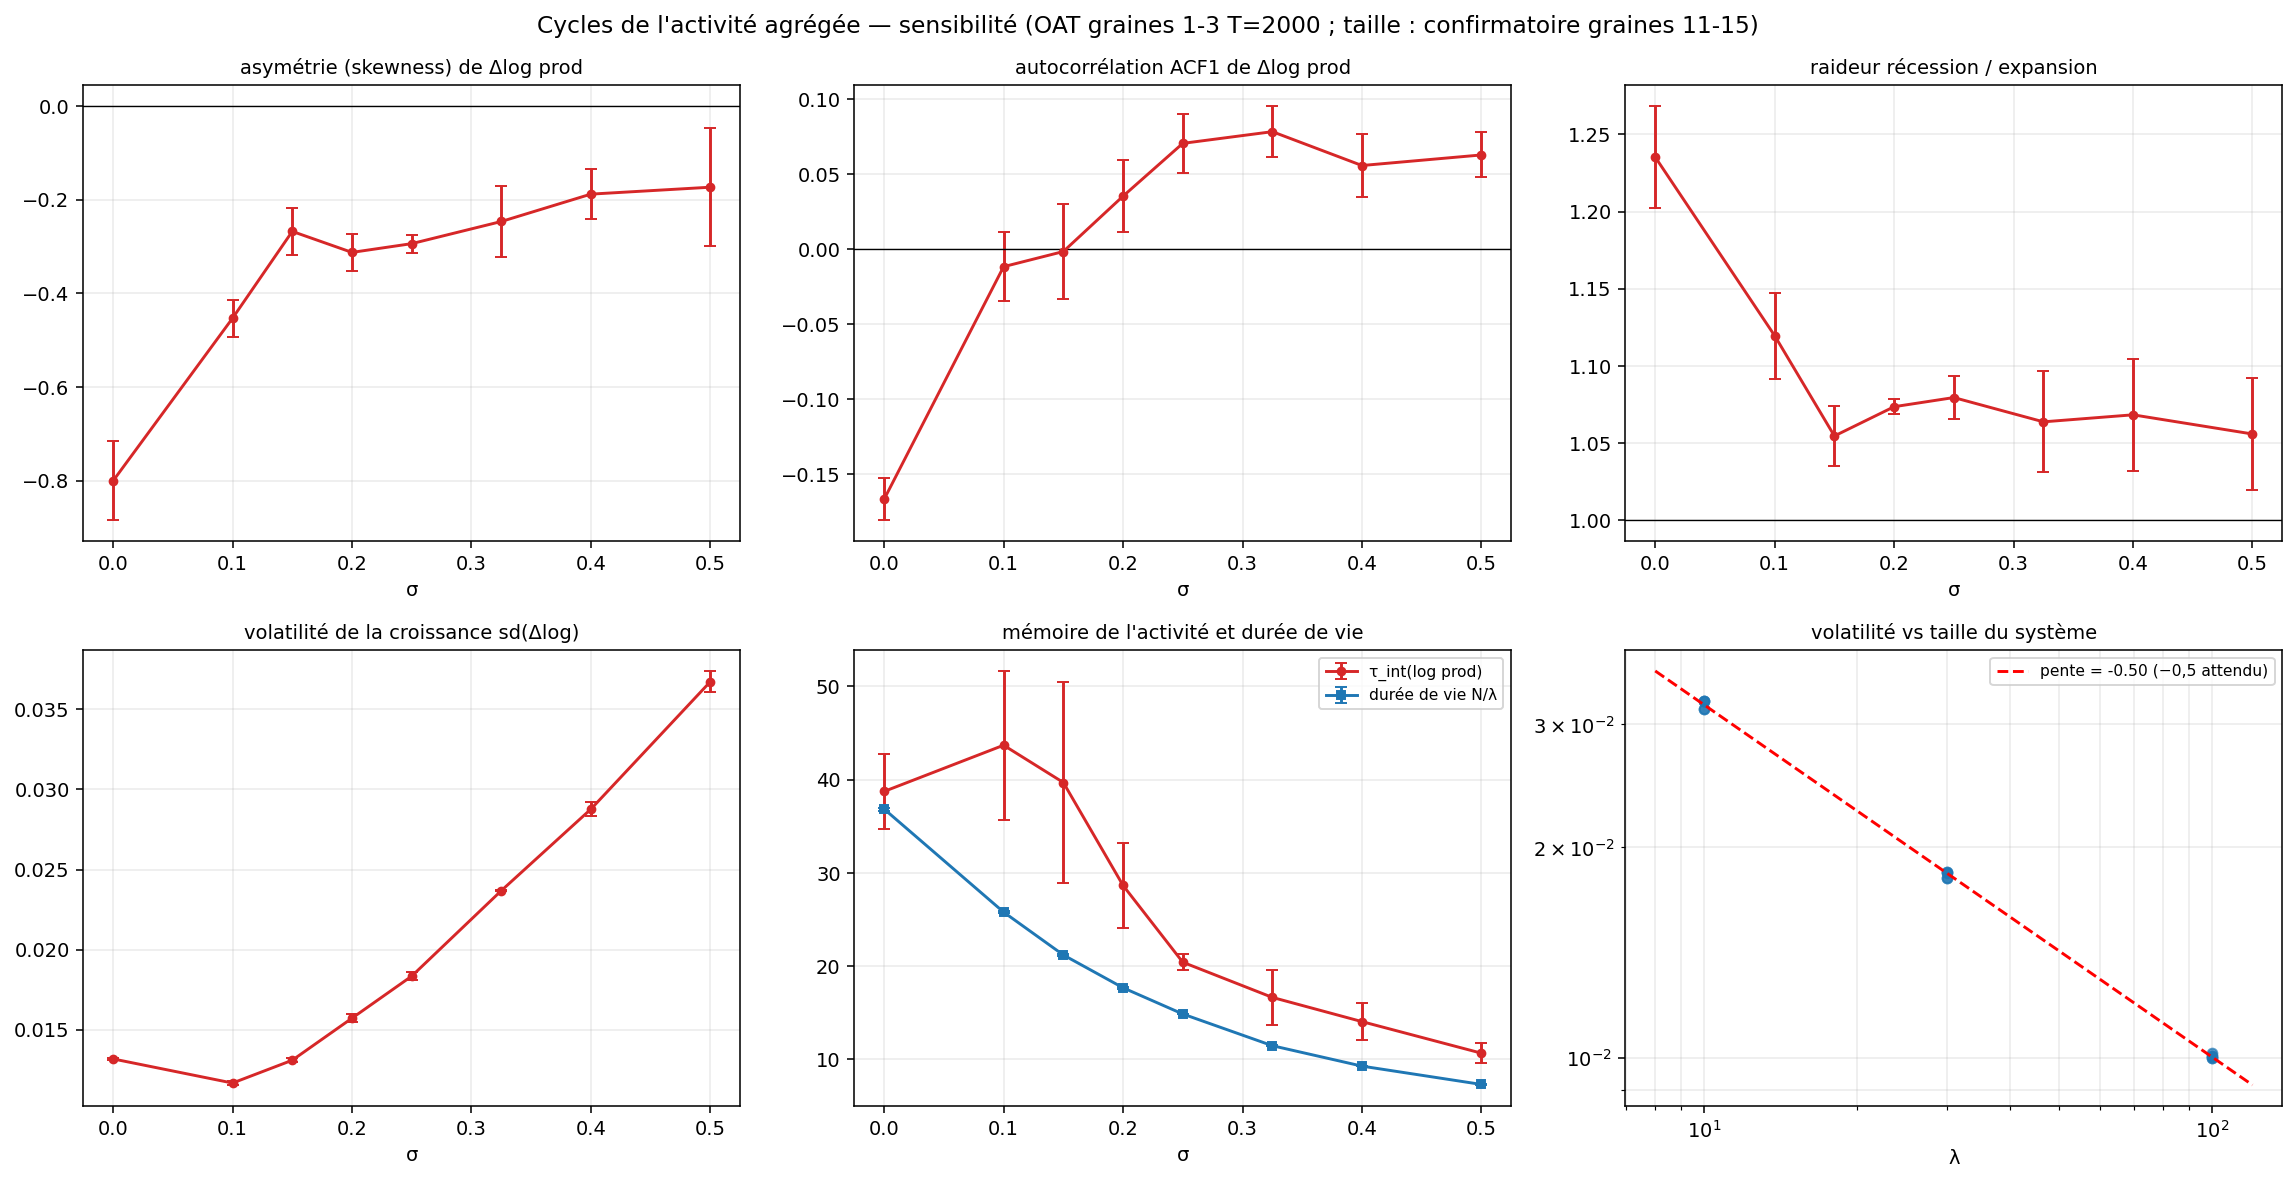
\includegraphics[width=\textwidth]{cycles_sensibilite.png}
\caption{Sensibilité des cycles (OAT, graines 1--3 ; dernier panneau :
cellules confirmatoires). Asymétrie, autocorrélation et raideur
relative des récessions le long de $\sigma$ ; volatilité de la
croissance (minimum intérieur vers $\sigma\simeq0{,}1$) ; temps de
mémoire de l'activité comparé à la durée de vie $N/\lambda$ ;
volatilité contre taille du système (pente log-log $-0{,}50$).}
\label{fig:cycles-sens}
\end{figure}

\begin{figure}[tbh]
\centering
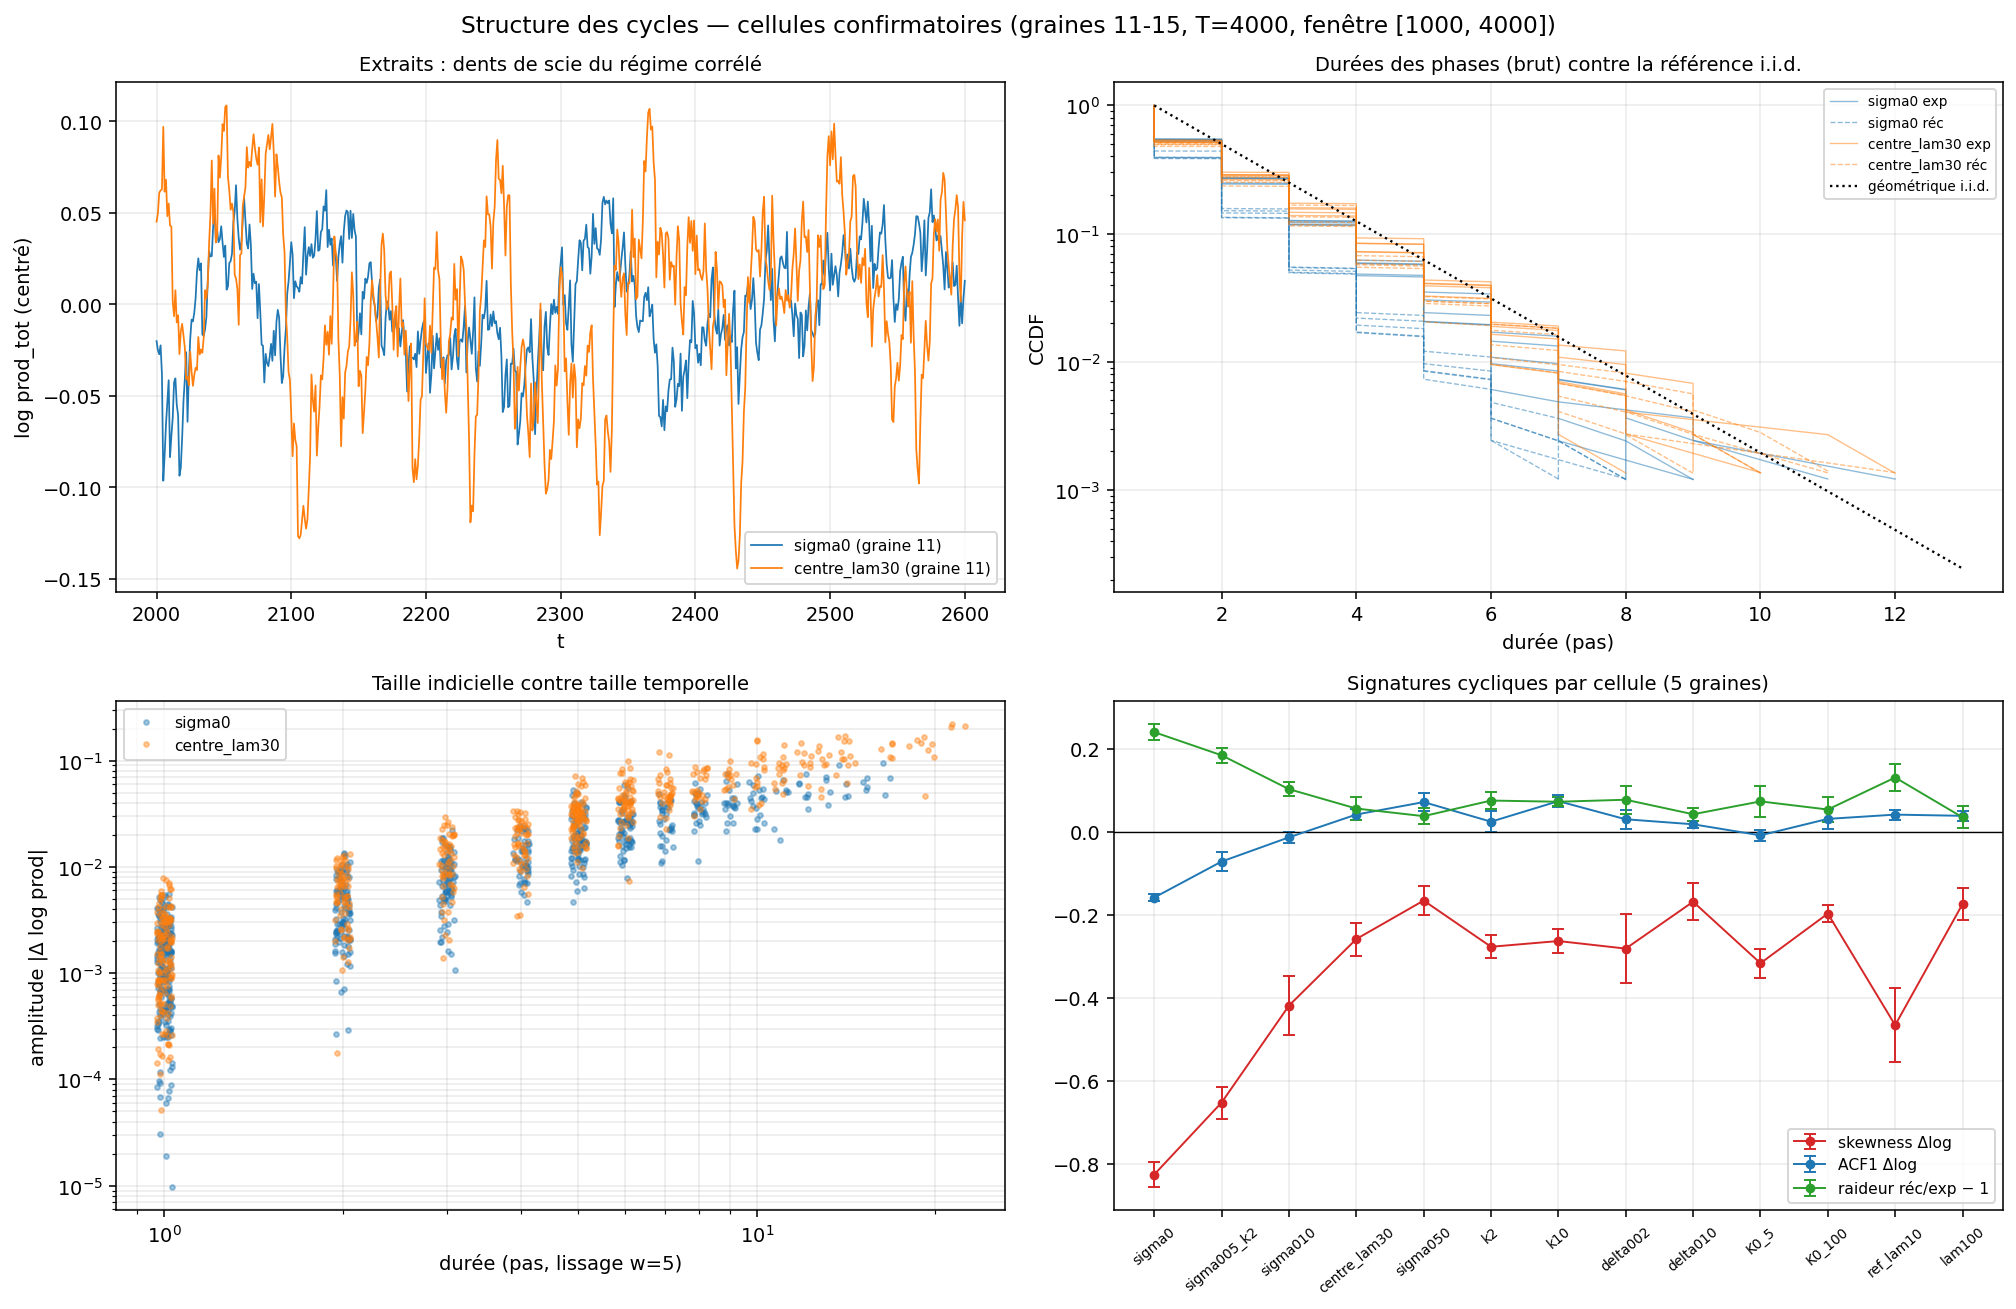
\includegraphics[width=\textwidth]{cycles_structure.png}
\caption{Structure des cycles (cellules confirmatoires). Extraits de
trajectoires (dents de scie du régime corrélé) ; CCDF des durées de
phases contre la référence géométrique i.i.d. (une courbe par graine) ;
taille indicielle contre taille temporelle (lissage $w=5$) ; signatures
par cellule.}
\label{fig:cycles-struct}
\end{figure}

\subsection{Fréquences et tailles : des cycles courts, sans phases
longues}

Faits (centre, 5 graines) : l'activité alterne $487\pm7$ épisodes par
millier de pas (un cycle complet expansion$+$récession dure en moyenne
$4{,}1$ pas) ; les durées moyennes sont $2{,}11\pm0{,}02$ pas
(expansions) et $2{,}00\pm0{,}06$ (récessions), avec des maxima de
$10$--$13$ pas sur 3\,000 pas observés : \textbf{aucune phase longue
n'existe} à l'échelle brute, et les CCDF des durées restent au niveau
ou en dessous de la référence géométrique i.i.d.
(figure~\ref{fig:cycles-struct}) — les phases sont plutôt \emph{plus
courtes} que le hasard, jamais plus longues. La taille indicielle croît
avec la taille temporelle (exposant descriptif
$\simeq1{,}7$--$1{,}8$ à $w=5$, stable entre cellules ; ce coefficient
décrit la sélection d'épisodes monotones et ne doit pas être lu comme
un exposant de Hurst). En lissant, des oscillations plus lentes
apparaissent (cycle moyen $9$--$10$ pas à $w=5$, $12$--$19$ à $w=25$,
maximal près du centre et réduit aux deux extrêmes de $\sigma$), mais
la mémoire vraie de l'activité est portée par
$\tau_{\mathrm{int}}$ : $23{,}5\pm0{,}6$ pas au centre,
$43{,}5\pm8{,}7$ à $\sigma=0$, $11{,}6$ à $\sigma=0{,}5$.

\paragraph{L'horloge des fluctuations est démographique.} Sur les 13
cellules confirmatoires, $\tau_{\mathrm{int}}$ suit la durée de vie
moyenne $N/\lambda$ (corrélation de rang $0{,}93$, rapport
$\tau_{\mathrm{int}}/(N/\lambda)$ entre $1{,}2$ et $1{,}8$ ;
figure~\ref{fig:cycles-sens}, panneau central bas) : le temps de
renouvellement de la population fixe la persistance des niveaux
d'activité. C'est le pendant temporel de la loi de Little.

\subsection{Volatilité : deux sources de bruit, un minimum intérieur}

La volatilité de la croissance $\mathrm{sd}(\Delta\log X)$ est pilotée
par $\sigma$ (PRCC $+0{,}97$) et par $K_0$ ($-0{,}81$), avec
$R^2_{\mathrm{CV}}=0{,}985$, et décroît avec la taille exactement comme
$\lambda^{-0{,}50}$ (mesuré $-0{,}50$, figure~\ref{fig:cycles-sens}) :
les fluctuations agrégées sont des sommes d'aléas quasi indépendants.
Fait non trivial : elle est \emph{non monotone} en $\sigma$, avec un
minimum intérieur vers $\sigma\simeq0{,}1$ ($0{,}0119$ contre
$0{,}0131$ à $\sigma=0$ et $0{,}0366$ à $\sigma=0{,}5$, valeurs OAT).
Lecture : à faible $\sigma$ le bruit agrégé est \emph{endogène} —
généré par les avalanches de faillites — tandis qu'à fort $\sigma$ il
est \emph{exogène} (chocs individuels) ; le minimum sépare les deux
régimes de bruit, au même endroit que la transition de propagation de
la section~\ref{sec:sigma}.

\subsection{Asymétrie de krach : une signature du régime corrélé, à
l'échelle des avalanches}

Faits confirmés (graines 11--15 ; 33 contrastes confirmés, 49 nuls
cohérents, 6 discordants mineurs, 24 sans contrepartie exploratoire) :

\begin{itemize}
\item la skewness de $\Delta\log X$ est \emph{toujours négative} (les
  baisses brutales dominent les hausses brutales) et son ampleur croît
  quand $\sigma$ décroît : $-0{,}26\pm0{,}04$ au centre,
  $-0{,}83\pm0{,}03$ à $\sigma=0$ ; elle s'atténue aussi avec la taille
  ($-0{,}46$ à $\lambda=10$, $-0{,}20$ à $\lambda=100$ : l'asymétrie de
  krach est un effet de taille finie des avalanches) ;
\item les récessions sont \emph{plus courtes} ($1{,}62$ contre
  $2{,}01$ pas à $\sigma=0$) et \emph{plus raides} que les expansions
  (rapport de pentes $1{,}24\pm0{,}02$ à $\sigma=0$, $1{,}06\pm0{,}03$
  au centre, $\to1{,}04$ à $\sigma=0{,}5$) — le profil « montée lente,
  chute brutale » des dents de scie visibles sur la
  figure~\ref{fig:cycles-struct} ;
\item l'autocorrélation des accroissements passe de $-0{,}16$
  ($\sigma=0$ : retour à la moyenne prononcé, chaque krach étant suivi
  de reconstruction) à $\simeq+0{,}05$ pour $\sigma\ge0{,}2$ : le
  croisement de zéro a lieu vers $\sigma\simeq0{,}15$, dans la zone de
  transition déjà identifiée.
\end{itemize}

Contrôle d'échelle : cette asymétrie vit à l'échelle brute, celle des
cascades intra-pas — le rapport de pentes tombe à $1{,}02$--$1{,}04$
dès $w=5$ et à $\simeq1{,}00$ à $w=25$. C'est une propriété
« microtemporelle » du mécanisme d'avalanche, pas une asymétrie de
grands cycles lissés.

\subsection{Portée pour M5}

Ces statistiques (volatilité, skewness, ACF1, taux d'épisodes,
$\tau_{\mathrm{int}}$, rapports de raideur) constituent la baseline
« conjoncturelle » de M4B : c'est contre elles que la future expérience
d'effet rebond de M5 — qui modifiera un paramètre \emph{en cours de
run} — devra comparer sa réponse dynamique et son contrefactuel
statique. La prédiction falsifiable centrale léguée à l'étude
analytique est le couple : $\tau_{\mathrm{int}}\propto$ durée de vie
(horloge démographique) et minimum intérieur de volatilité à la
frontière bruit endogène/exogène.

\section{Résultats négatifs et effets non confirmés}
\label{sec:negatifs}

Conformément au protocole, nous listons ce qui n'a \emph{pas} été
observé ou confirmé :

\begin{itemize}
\item \textbf{Aucune extinction dynamique, aucune croissance soutenue,
  aucune censure} par le garde-fou dans tout l'espace exploré
  (section~\ref{sec:regimes}).
\item \textbf{Micro-dépendances de la démographie en $\lambda$ non
  confirmées} : l'exploration suggérait $N/\lambda$ légèrement
  décroissant de $\lambda=10$ à $100$ ($-1$ à $-2\,\%$) ; la
  confirmation donne des signes opposés et de plus faibles amplitudes
  ($+0{,}163\pm0{,}053$ à $\lambda=10$, $-0{,}017\pm0{,}027$ à
  $\lambda=100$). Verdict : pas de dépendance fiable ; l'intensivité
  est la description correcte.
\item \textbf{Coupure $\hat s_c$ à $k=2$ non confirmée en amplitude}
  (contraste exploratoire $-3{,}2$, confirmé $+6{,}0\pm2{,}8$) : la
  coupure est la métrique la plus bruitée (variance graines $17\,\%$)
  et ne doit être lue qu'à travers son scaling en $\lambda$.
\item \textbf{Profondeur maximale de cascade non prédictible} par les
  paramètres ($R^2_{\mathrm{CV}}=0{,}09$ ; $72\,\%$ de variance
  stochastique) : nous ne rapportons aucune conclusion paramétrique sur
  cette métrique extrême.
\item \textbf{Trois amplitudes décalées} (signe correct, rapport hors
  $[0{,}5;2]$) : dette/capital à $\sigma=0$, coupure à $K_0=100$,
  prêts par tête à $k=2$ — toutes portées par les métriques les plus
  variables ; aucune n'inverse une conclusion.
\end{itemize}

\section{Recommandations de réduction pour M5}
\label{sec:reduction}

Rappel : la présente étude n'implémente aucune réduction ; les
décisions appartiennent à la conception de M5.

\begin{enumerate}
\item \textbf{$\sigma$, $k$, $K_0$ : à conserver comme paramètres
  scientifiques.} Ils portent des effets forts, distincts et
  confirmés sur trois familles de réponses différentes (démographie ;
  inégalités et statistique fine ; protection démographique).
\item \textbf{$\delta$ : candidat à l'absorption par adimensionnement,
  avec une réserve explicite.} À $\sigma\ge0{,}2$, $\delta$ agit comme
  l'échelle du capital (point fixe individuel $K^\ast=(1/\delta)^2$
  avec $\alpha=1$) : M5 pourrait le fixer par convention d'unités
  (p.~ex. mesurer $K$ en unités de $K^\ast$, ce qui ferait de
  $K_0/K^\ast$ le vrai paramètre) — à condition de vérifier
  analytiquement que le taux du marché et le service des intérêts se
  renormalisent de même. Deux faits empêchent une suppression
  aveugle : l'effet démographique modéré mais réel de $\delta$
  ($N/\lambda$ : $13{,}5\to16{,}9$ sur la plage) et son module de
  propagation dans le régime $\sigma<0{,}15$.
\item \textbf{$\lambda$ : à traiter comme taille du système, pas comme
  levier économique.} Toutes les grandeurs intensives en sont
  indépendantes ; seuls les effets de taille finie (coupure, maximum,
  susceptibilité) en dépendent, avec des pentes désormais chiffrées.
  L'extinction d'amorçage $e^{-\lambda}$ doit être traitée comme une
  condition initiale, pas comme un phénomène.
\item \textbf{\code{pop\_max}, tolérances, $\alpha=1$ : conventions
  confirmées.} Le garde-fou n'a jamais été actif ; le maintenir
  n'introduit aucun biais dans les plages explorées.
\item \textbf{Simplifications de mesure} : la profondeur maximale et la
  coupure ajustée sont trop bruitées pour servir d'observables de
  pilotage ; privilégier $b$, $\hat\alpha$ (avec taille de système
  déclarée), la susceptibilité et $N/\lambda$.
\end{enumerate}

\section{Feuille de route M5 (hors périmètre de la présente étude)}
\label{sec:m5}

\subsection{Exposant de concavité $\gamma$}

M5 introduira $F_\gamma(K)=\alpha K^\gamma$, $0<\gamma<1$
($\gamma=1/2$ : cas M4B). Les baselines utiles pour isoler son effet
sont posées ici : les valeurs de référence de la
table~\ref{tab:centre} ; l'échelle individuelle attendue
$K^\ast=(\alpha/\delta)^{1/(1-\gamma)}$, qui redonne $(1/\delta)^2$ à
$\gamma=1/2$ et devrait gouverner le capital par tête ; le produit
marginal $\gamma\alpha K^{\gamma-1}$ qui fixera les taux du marché ;
et les signatures de taille finie de la figure~\ref{fig:scaling}, à
re-mesurer à $\gamma\ne1/2$ pour tester si l'exposant $\alpha$ des
avalanches et le plateau $b\simeq0{,}30$ sont bien institutionnels
(règles du marché) plutôt que productifs.

\subsection{Variation dynamique et effet rebond}

La présente étude n'a fait varier que des constantes entre runs et ne
peut donc rien affirmer sur un effet rebond au sens de Sorrell et
Dimitropoulos (2008). Pour le mesurer, M5 devra définir : (i) une
\emph{amélioration d'efficacité} (candidats naturels : $\alpha$ ou
$\gamma$, modifiés en cours de run) ; (ii) la \emph{ressource}
consommée et le \emph{service} rendu — dans M4B, la production
$\sum\sqrt{K_i}$ et le capital total jouent ces rôles mais ne sont pas
distingués d'une consommation ; (iii) un \emph{contrefactuel statique}
« sans rebond » simulé en parallèle (mêmes graines, paramètre gelé),
auquel comparer la réponse dynamique. Les séries nécessaires
(production, capital, flux d'intérêts, volumes de crédit, démographie)
sont déjà enregistrées par le moteur à chaque pas ; il manque
uniquement la machinerie de changement de paramètre en cours de run et
la définition du service. Une simple hausse de population ou de
production après un changement ne suffira pas : il faudra l'écart au
contrefactuel.

\subsection{Étude analytique}

Les faits empiriques suivants contraignent déjà la théorie à venir et
lui fournissent des prédictions falsifiables :

\begin{itemize}
\item \emph{Démographie} : $N/\lambda=\E[\text{âge au décès}]$ (loi de
  Little, vérifiée partout) ; l'analyse doit produire l'espérance de
  durée de vie en fonction de $(\sigma,K_0,\delta,k)$ — convexité en
  $\sigma$, log-linéarité en $K_0$, croissance modérée en $\delta$.
\item \emph{Point fixe du capital} : sans crédit,
  $\delta K=\alpha\sqrt K$ donne $K^\ast=(\alpha/\delta)^2$ ; le
  capital par tête observé ($98{,}8$~J au centre) est bien en dessous
  ($400$~J), à hauteur de l'âge fini des entités — l'analyse de la
  dynamique moyenne doit expliquer ce facteur.
\item \emph{Stationnarité inconditionnelle} : aucune bifurcation
  extinction/croissance dans les plages explorées ; l'état vide n'est
  accessible que par l'amorçage ($e^{-\lambda}$). Une théorie qui
  prédirait une transition de phase démographique dans ces plages
  serait falsifiée.
\item \emph{Bilans} : la mortalité est entièrement pilotée par la
  valeur nette dans les plages étudiées (canal de liquidité silencieux
  sous $\sigma\simeq0{,}85$) ; la profondeur médiane du trou
  d'insolvabilité vaut $-8{,}6\,\%\pm0{,}2$ du capital par tête le long
  de $\delta$, $K_0$, $k$ et $\lambda$, et ne dépend que de $\sigma$ —
  deux prédictions falsifiables directes pour la théorie ; le cycle de
  vie débiteur$\to$créancier (plongeon initial à $x/K\simeq-0{,}85$,
  remontée par les intérêts composés) devrait se déduire de la règle de
  marché et du service des intérêts.
\item \emph{Cascades} : loi tronquée avec
  $\alpha_\infty\simeq2{,}31$, $\hat s_c$ croissant vite avec
  $\lambda$ (pente $\simeq1{,}5$ sur $[10,30]$),
  $s_{\max}\propto\lambda^{0{,}58}$,
  $\chi\propto\lambda^{0{,}51}$ ; plateau institutionnel
  $b\simeq0{,}30$ dont la théorie doit dériver la valeur depuis la
  règle « un round par tête », et ses deux conditions de sortie
  ($\sigma\lesssim0{,}2$, grand $k$).
\item \emph{Distinction bifurcation / transitoire / censure} : dans
  M4B, les trois diagnostics prévus (plafonds multiples, pentes,
  encadrement de frontière) n'ont jamais eu à s'appliquer ; M5 devra
  les conserver au cas où $\gamma>1/2$ ouvrirait un régime de
  croissance réelle.
\end{itemize}

\section{Limites}
\label{sec:limites}

(i) Les plages, bien qu'élargies par les sondes ($\sigma$ jusqu'à 1,
$\delta$ jusqu'à $0{,}01$, $K_0$ de 2 à 200), restent finies ; nous ne
nous prononçons pas au-delà, notamment pour $\delta\to0$ strict ou
$K_0\to\infty$. (ii) L'estimation de la coupure est peu fiable cellule
par cellule (variance graines $17\,\%$) ; seules ses tendances de
taille sont robustes ; la pente $1{,}5$ de $\hat s_c(\lambda)$ ne
repose que sur deux tailles identifiables. (iii) Le plan LHS est un
plan de screening : les PRCC et importances n'ont pas le statut
d'indices de Sobol. (iv) Les horizons vont jusqu'à $T=8000$ ; des
métastabilités au-delà ne peuvent être exclues, quoique rien ne les
suggère. (v) Les ajustements de lois portent sur $s\ge2$ ; les morts
isolées (taille 1), majoritaires, sont décrites par le taux de
mortalité, pas par la loi de puissance. (vi) La comparaison
exploration/confirmation repose sur des panels de graines disjoints
mais de petite taille (3 et 5) ; les intervalles reflètent cette
taille.

\section{Conclusion}

La sensibilité de M4B se résume en une phrase par paramètre : $\sigma$
fixe la durée de vie et l'exposition, $k$ fixe les inégalités de
capital et le détail des cascades, $K_0$ protège les jeunes, $\delta$
fixe l'unité de capital (sauf à très faible bruit), $\lambda$ fixe la
taille du système ; c'est la valeur nette — non le capital — qui
porte l'inégalité, la mémoire du cycle de vie et la totalité de la
mortalité dans les plages étudiées ; et la conjoncture agrégée bat au
rythme du renouvellement démographique, avec pour seule signature
singulière l'asymétrie de krach héritée des avalanches. Le modèle est partout stationnaire, ses signatures critiques
(loi tronquée, coupure croissante avec la taille,
$\alpha_\infty\simeq2{,}31$, plateau $b\simeq0{,}30$) sont robustes aux
graines, aux fenêtres et aux horizons, et ses seules « frontières »
sont un artefact d'amorçage et une transition douce vers le régime
corrélé sans choc. Ces éléments, avec les baselines chiffrées de la
table~\ref{tab:centre}, forment le socle de comparaison pour M5.

\appendix

\section{Traçabilité}
\label{sec:annexe}

Chaque valeur et figure de ce rapport provient des runs listés
ci-dessous (594 runs distincts ; une cellule partagée par plusieurs
plans apparaît sous chacun, 680 entrées). Les figures OAT/LHS/coupes
agrègent les plans du même nom ; les tables~\ref{tab:centre} et
\ref{tab:lois} et les figures de confirmation proviennent des lots
Simulation Lab (préfixe de plan « confirm »), consultables dans
l'interface avec leurs figures et marqués « à conserver ».

% Annexe générée par scripts/make_annexe.py — ne pas éditer à la main.
{\scriptsize\setlength{\tabcolsep}{3.5pt}
\begin{longtable}{@{}llrrrrrrrl@{}}
\toprule
run\_id & plan & $\lambda$ & $\delta$ & $\sigma$ & $K_0$ & $k$ & graine & $T$ & statut \\
\midrule
\endhead
\code{m4b\_797485073afe} & benchmark & 10 & 0.05 & 0.25 & 25 & 3 & 0 & 2000 & ok \\
\code{m4b\_8efd385078ae} & benchmark & 30 & 0.05 & 0.25 & 25 & 3 & 0 & 2000 & ok \\
\code{m4b\_392895f517cd} & benchmark & 100 & 0.05 & 0.25 & 25 & 3 & 0 & 2000 & ok \\
\code{m4b\_2cb7bc83f1d9} & benchmark & 30 & 0.05 & 0.25 & 25 & 3 & 0 & 2000 & ok \\
\code{m4b\_04c4cd570599} & benchmark & 10 & 0.02 & 0.1 & 25 & 3 & 0 & 2000 & ok \\
\code{m4b\_36486750246d} & benchmark & 10 & 0.05 & 0.25 & 25 & 3 & 0 & 2000 & ok \\
\code{m4b\_f1f11729d707} & pilotes & 30 & 0.02 & 0.1 & 25 & 3 & 1 & 2000 & ok \\
\code{m4b\_63b4b58b5c5e} & pilotes & 30 & 0.02 & 0.1 & 25 & 3 & 2 & 2000 & ok \\
\code{m4b\_7ff8a4b9c628} & pilotes & 30 & 0.02 & 0.5 & 25 & 3 & 1 & 2000 & ok \\
\code{m4b\_0b15f46fa1df} & pilotes & 30 & 0.02 & 0.5 & 25 & 3 & 2 & 2000 & ok \\
\code{m4b\_c5dd2c6050e7} & pilotes & 30 & 0.1 & 0.1 & 25 & 3 & 1 & 2000 & ok \\
\code{m4b\_2180a4bc480e} & pilotes & 30 & 0.1 & 0.1 & 25 & 3 & 2 & 2000 & ok \\
\code{m4b\_83524c6aac7c} & pilotes & 30 & 0.1 & 0.5 & 25 & 3 & 1 & 2000 & ok \\
\code{m4b\_c032337f5278} & pilotes & 30 & 0.1 & 0.5 & 25 & 3 & 2 & 2000 & ok \\
\code{m4b\_35a10e8501c4} & pilotes & 30 & 0.05 & 0.25 & 5 & 3 & 1 & 2000 & ok \\
\code{m4b\_a8039a7bf647} & pilotes & 30 & 0.05 & 0.25 & 5 & 3 & 2 & 2000 & ok \\
\code{m4b\_070fbcacbeda} & pilotes & 30 & 0.05 & 0.25 & 100 & 3 & 1 & 2000 & ok \\
\code{m4b\_73aa94bd63b4} & pilotes & 30 & 0.05 & 0.25 & 100 & 3 & 2 & 2000 & ok \\
\code{m4b\_4152360a697e} & pilotes & 30 & 0.05 & 0.25 & 25 & 2 & 1 & 2000 & ok \\
\code{m4b\_76ee2b65c2bd} & pilotes & 30 & 0.05 & 0.25 & 25 & 2 & 2 & 2000 & ok \\
\code{m4b\_815693ccb3ee} & pilotes & 30 & 0.05 & 0.25 & 25 & 10 & 1 & 2000 & ok \\
\code{m4b\_6155b9db63b7} & pilotes & 30 & 0.05 & 0.25 & 25 & 10 & 2 & 2000 & ok \\
\code{m4b\_4389d08d5eef} & pilotes & 30 & 0.05 & 0 & 25 & 3 & 1 & 2000 & ok \\
\code{m4b\_334b58e2a70f} & pilotes & 30 & 0.05 & 0 & 25 & 3 & 2 & 2000 & ok \\
\code{m4b\_d9ad462f97e3} & pilotes & 30 & 0.05 & 0 & 25 & 2 & 1 & 2000 & ok \\
\code{m4b\_8614a4e0fa49} & pilotes & 30 & 0.05 & 0 & 25 & 2 & 2 & 2000 & ok \\
\code{m4b\_8d72e0e2fb28} & pilotes & 30 & 0.02 & 0 & 25 & 3 & 1 & 2000 & ok \\
\code{m4b\_d4dfdc238338} & pilotes & 30 & 0.02 & 0 & 25 & 3 & 2 & 2000 & ok \\
\code{m4b\_223ee698ee8a} & pilotes & 30 & 0.05 & 0.25 & 25 & 3 & 1 & 2000 & ok \\
\code{m4b\_9433691bedb8} & pilotes & 30 & 0.05 & 0.25 & 25 & 3 & 2 & 2000 & ok \\
\code{m4b\_0ca44bdda123} & pilotes & 30 & 0.1 & 0.5 & 5 & 3 & 1 & 2000 & ok \\
\code{m4b\_5bc5958dd40b} & pilotes & 30 & 0.1 & 0.5 & 5 & 3 & 2 & 2000 & ok \\
\code{m4b\_3373fcbcc8a5} & pilotes & 30 & 0.05 & 0.25 & 25 & 3 & 1 & 4000 & ok \\
\code{m4b\_225424622d91} & pilotes & 30 & 0.05 & 0.25 & 25 & 3 & 2 & 4000 & ok \\
\code{m4b\_4e761d701121} & pilotes & 30 & 0.02 & 0.1 & 25 & 3 & 1 & 8000 & ok \\
\code{m4b\_8c24588f6433} & pilotes & 100 & 0.02 & 0.1 & 25 & 3 & 1 & 2000 & ok \\
\code{m4b\_7e7dad60452f} & pilotes2 & 30 & 0.05 & 0.6 & 25 & 3 & 1 & 2000 & ok \\
\code{m4b\_a43d69c1d859} & pilotes2 & 30 & 0.05 & 0.6 & 25 & 3 & 2 & 2000 & ok \\
\code{m4b\_719411d80c90} & pilotes2 & 30 & 0.05 & 0.7 & 25 & 3 & 1 & 2000 & ok \\
\code{m4b\_b254dcc3b896} & pilotes2 & 30 & 0.05 & 0.7 & 25 & 3 & 2 & 2000 & ok \\
\code{m4b\_9644f4000a16} & pilotes2 & 30 & 0.05 & 0.85 & 25 & 3 & 1 & 2000 & ok \\
\code{m4b\_bd2ccb4f50b3} & pilotes2 & 30 & 0.05 & 0.85 & 25 & 3 & 2 & 2000 & ok \\
\code{m4b\_e70a79d129ed} & pilotes2 & 30 & 0.05 & 1 & 25 & 3 & 1 & 2000 & ok \\
\code{m4b\_b275a90d600c} & pilotes2 & 30 & 0.05 & 1 & 25 & 3 & 2 & 2000 & ok \\
\code{m4b\_7f5be71bde33} & pilotes2 & 30 & 0.01 & 0.05 & 25 & 3 & 1 & 2000 & ok \\
\code{m4b\_7690fbf4f754} & pilotes2 & 30 & 0.01 & 0.05 & 25 & 3 & 2 & 2000 & ok \\
\code{m4b\_e34e64d8e486} & pilotes2 & 30 & 0.01 & 0.25 & 25 & 3 & 1 & 2000 & ok \\
\code{m4b\_bf8b7868a980} & pilotes2 & 30 & 0.01 & 0.25 & 25 & 3 & 2 & 2000 & ok \\
\code{m4b\_2db90273aff4} & pilotes2 & 30 & 0.05 & 0.25 & 2 & 3 & 1 & 2000 & ok \\
\code{m4b\_9906d8cc2c20} & pilotes2 & 30 & 0.05 & 0.25 & 2 & 3 & 2 & 2000 & ok \\
\code{m4b\_5065ba3bf84e} & pilotes2 & 30 & 0.05 & 0.25 & 200 & 3 & 1 & 2000 & ok \\
\code{m4b\_5c72d7fe2ae0} & pilotes2 & 30 & 0.05 & 0.25 & 200 & 3 & 2 & 2000 & ok \\
\code{m4b\_99f85acb771b} & oat & 30 & 0.02 & 0.25 & 25 & 3 & 1 & 2000 & ok \\
\code{m4b\_6f10c4ffdf3f} & oat & 30 & 0.02 & 0.25 & 25 & 3 & 2 & 2000 & ok \\
\code{m4b\_cbf510d44807} & oat & 30 & 0.02 & 0.25 & 25 & 3 & 3 & 2000 & ok \\
\code{m4b\_7e48d343025a} & oat & 30 & 0.03 & 0.25 & 25 & 3 & 1 & 2000 & ok \\
\code{m4b\_f9736ede0c29} & oat & 30 & 0.03 & 0.25 & 25 & 3 & 2 & 2000 & ok \\
\code{m4b\_6e9d00e9fbfe} & oat & 30 & 0.03 & 0.25 & 25 & 3 & 3 & 2000 & ok \\
\code{m4b\_223ee698ee8a} & oat & 30 & 0.05 & 0.25 & 25 & 3 & 1 & 2000 & ok \\
\code{m4b\_9433691bedb8} & oat & 30 & 0.05 & 0.25 & 25 & 3 & 2 & 2000 & ok \\
\code{m4b\_1d87c9ae13e4} & oat & 30 & 0.05 & 0.25 & 25 & 3 & 3 & 2000 & ok \\
\code{m4b\_44e7b6d9479c} & oat & 30 & 0.07 & 0.25 & 25 & 3 & 1 & 2000 & ok \\
\code{m4b\_9c969e4e337c} & oat & 30 & 0.07 & 0.25 & 25 & 3 & 2 & 2000 & ok \\
\code{m4b\_f0eaa06cc865} & oat & 30 & 0.07 & 0.25 & 25 & 3 & 3 & 2000 & ok \\
\code{m4b\_40ab5c70c607} & oat & 30 & 0.1 & 0.25 & 25 & 3 & 1 & 2000 & ok \\
\code{m4b\_9355e219bada} & oat & 30 & 0.1 & 0.25 & 25 & 3 & 2 & 2000 & ok \\
\code{m4b\_c50e5463b057} & oat & 30 & 0.1 & 0.25 & 25 & 3 & 3 & 2000 & ok \\
\code{m4b\_4389d08d5eef} & oat & 30 & 0.05 & 0 & 25 & 3 & 1 & 2000 & ok \\
\code{m4b\_334b58e2a70f} & oat & 30 & 0.05 & 0 & 25 & 3 & 2 & 2000 & ok \\
\code{m4b\_16e9ffc35a50} & oat & 30 & 0.05 & 0 & 25 & 3 & 3 & 2000 & ok \\
\code{m4b\_1b8e7e58a7d1} & oat & 30 & 0.05 & 0.1 & 25 & 3 & 1 & 2000 & ok \\
\code{m4b\_a265a0190ae2} & oat & 30 & 0.05 & 0.1 & 25 & 3 & 2 & 2000 & ok \\
\code{m4b\_1275f4990c98} & oat & 30 & 0.05 & 0.1 & 25 & 3 & 3 & 2000 & ok \\
\code{m4b\_923b5e0a754c} & oat & 30 & 0.05 & 0.15 & 25 & 3 & 1 & 2000 & ok \\
\code{m4b\_be4ae4164d04} & oat & 30 & 0.05 & 0.15 & 25 & 3 & 2 & 2000 & ok \\
\code{m4b\_1402884dc872} & oat & 30 & 0.05 & 0.15 & 25 & 3 & 3 & 2000 & ok \\
\code{m4b\_f3530dbcf367} & oat & 30 & 0.05 & 0.2 & 25 & 3 & 1 & 2000 & ok \\
\code{m4b\_83ce80c2bd57} & oat & 30 & 0.05 & 0.2 & 25 & 3 & 2 & 2000 & ok \\
\code{m4b\_9887e01d6cff} & oat & 30 & 0.05 & 0.2 & 25 & 3 & 3 & 2000 & ok \\
\code{m4b\_aa8c18f6b827} & oat & 30 & 0.05 & 0.325 & 25 & 3 & 1 & 2000 & ok \\
\code{m4b\_63fc88093f48} & oat & 30 & 0.05 & 0.325 & 25 & 3 & 2 & 2000 & ok \\
\code{m4b\_37e927b1de27} & oat & 30 & 0.05 & 0.325 & 25 & 3 & 3 & 2000 & ok \\
\code{m4b\_3ddd0930487d} & oat & 30 & 0.05 & 0.4 & 25 & 3 & 1 & 2000 & ok \\
\code{m4b\_74004546d4de} & oat & 30 & 0.05 & 0.4 & 25 & 3 & 2 & 2000 & ok \\
\code{m4b\_6de962cbe8c9} & oat & 30 & 0.05 & 0.4 & 25 & 3 & 3 & 2000 & ok \\
\code{m4b\_cb087c61e004} & oat & 30 & 0.05 & 0.5 & 25 & 3 & 1 & 2000 & ok \\
\code{m4b\_23acad9dae6f} & oat & 30 & 0.05 & 0.5 & 25 & 3 & 2 & 2000 & ok \\
\code{m4b\_d54308beb42a} & oat & 30 & 0.05 & 0.5 & 25 & 3 & 3 & 2000 & ok \\
\code{m4b\_35a10e8501c4} & oat & 30 & 0.05 & 0.25 & 5 & 3 & 1 & 2000 & ok \\
\code{m4b\_a8039a7bf647} & oat & 30 & 0.05 & 0.25 & 5 & 3 & 2 & 2000 & ok \\
\code{m4b\_39343567e1f9} & oat & 30 & 0.05 & 0.25 & 5 & 3 & 3 & 2000 & ok \\
\code{m4b\_c602a838a7f1} & oat & 30 & 0.05 & 0.25 & 10 & 3 & 1 & 2000 & ok \\
\code{m4b\_d5227166331c} & oat & 30 & 0.05 & 0.25 & 10 & 3 & 2 & 2000 & ok \\
\code{m4b\_5f4c83d1cc97} & oat & 30 & 0.05 & 0.25 & 10 & 3 & 3 & 2000 & ok \\
\code{m4b\_0ab9802382e9} & oat & 30 & 0.05 & 0.25 & 50 & 3 & 1 & 2000 & ok \\
\code{m4b\_cdf5d6a63b10} & oat & 30 & 0.05 & 0.25 & 50 & 3 & 2 & 2000 & ok \\
\code{m4b\_c6b2b42aefee} & oat & 30 & 0.05 & 0.25 & 50 & 3 & 3 & 2000 & ok \\
\code{m4b\_070fbcacbeda} & oat & 30 & 0.05 & 0.25 & 100 & 3 & 1 & 2000 & ok \\
\code{m4b\_73aa94bd63b4} & oat & 30 & 0.05 & 0.25 & 100 & 3 & 2 & 2000 & ok \\
\code{m4b\_f5d52a671696} & oat & 30 & 0.05 & 0.25 & 100 & 3 & 3 & 2000 & ok \\
\code{m4b\_4152360a697e} & oat & 30 & 0.05 & 0.25 & 25 & 2 & 1 & 2000 & ok \\
\code{m4b\_76ee2b65c2bd} & oat & 30 & 0.05 & 0.25 & 25 & 2 & 2 & 2000 & ok \\
\code{m4b\_1670f6a5f468} & oat & 30 & 0.05 & 0.25 & 25 & 2 & 3 & 2000 & ok \\
\code{m4b\_f85ef5506838} & oat & 30 & 0.05 & 0.25 & 25 & 4 & 1 & 2000 & ok \\
\code{m4b\_ea1688044052} & oat & 30 & 0.05 & 0.25 & 25 & 4 & 2 & 2000 & ok \\
\code{m4b\_23e65c27433b} & oat & 30 & 0.05 & 0.25 & 25 & 4 & 3 & 2000 & ok \\
\code{m4b\_ae520266d772} & oat & 30 & 0.05 & 0.25 & 25 & 6 & 1 & 2000 & ok \\
\code{m4b\_edfaf765def4} & oat & 30 & 0.05 & 0.25 & 25 & 6 & 2 & 2000 & ok \\
\code{m4b\_1115f794fa8e} & oat & 30 & 0.05 & 0.25 & 25 & 6 & 3 & 2000 & ok \\
\code{m4b\_815693ccb3ee} & oat & 30 & 0.05 & 0.25 & 25 & 10 & 1 & 2000 & ok \\
\code{m4b\_6155b9db63b7} & oat & 30 & 0.05 & 0.25 & 25 & 10 & 2 & 2000 & ok \\
\code{m4b\_111f5ff3a21d} & oat & 30 & 0.05 & 0.25 & 25 & 10 & 3 & 2000 & ok \\
\code{m4b\_02364a291262} & oat & 10 & 0.05 & 0.25 & 25 & 3 & 1 & 2000 & ok \\
\code{m4b\_d641da597a6d} & oat & 10 & 0.05 & 0.25 & 25 & 3 & 2 & 2000 & ok \\
\code{m4b\_0d5cdd2d0b98} & oat & 10 & 0.05 & 0.25 & 25 & 3 & 3 & 2000 & ok \\
\code{m4b\_7b9b4988f289} & oat & 100 & 0.05 & 0.25 & 25 & 3 & 1 & 2000 & ok \\
\code{m4b\_b4bacbb71e13} & oat & 100 & 0.05 & 0.25 & 25 & 3 & 2 & 2000 & ok \\
\code{m4b\_97c523ee360f} & oat & 100 & 0.05 & 0.25 & 25 & 3 & 3 & 2000 & ok \\
\code{m4b\_4ae10eca1d55} & lambda\_ext & 1 & 0.05 & 0.25 & 25 & 3 & 1 & 2000 & ok \\
\code{m4b\_5a41f992ac5d} & lambda\_ext & 1 & 0.05 & 0.25 & 25 & 3 & 2 & 2000 & extinction \\
\code{m4b\_d0636ba0350b} & lambda\_ext & 1 & 0.05 & 0.25 & 25 & 3 & 3 & 2000 & extinction \\
\code{m4b\_5f27c0e30e91} & lambda\_ext & 1 & 0.05 & 0.5 & 25 & 3 & 1 & 2000 & ok \\
\code{m4b\_eb78551dd21a} & lambda\_ext & 1 & 0.05 & 0.5 & 25 & 3 & 2 & 2000 & extinction \\
\code{m4b\_e42400705557} & lambda\_ext & 1 & 0.05 & 0.5 & 25 & 3 & 3 & 2000 & extinction \\
\code{m4b\_eef15617eaf0} & lambda\_ext & 1 & 0.05 & 1 & 25 & 3 & 1 & 2000 & ok \\
\code{m4b\_42731353455a} & lambda\_ext & 1 & 0.05 & 1 & 25 & 3 & 2 & 2000 & extinction \\
\code{m4b\_1749ae4ecc0c} & lambda\_ext & 1 & 0.05 & 1 & 25 & 3 & 3 & 2000 & extinction \\
\code{m4b\_360db3e7fe18} & lambda\_ext & 2 & 0.05 & 0.25 & 25 & 3 & 1 & 2000 & ok \\
\code{m4b\_aaeb331c6434} & lambda\_ext & 2 & 0.05 & 0.25 & 25 & 3 & 2 & 2000 & ok \\
\code{m4b\_c1e0f7349e8b} & lambda\_ext & 2 & 0.05 & 0.25 & 25 & 3 & 3 & 2000 & extinction \\
\code{m4b\_acabab625d76} & lambda\_ext & 2 & 0.05 & 0.5 & 25 & 3 & 1 & 2000 & ok \\
\code{m4b\_c16b8914a4f7} & lambda\_ext & 2 & 0.05 & 0.5 & 25 & 3 & 2 & 2000 & ok \\
\code{m4b\_d28af555ed5e} & lambda\_ext & 2 & 0.05 & 0.5 & 25 & 3 & 3 & 2000 & extinction \\
\code{m4b\_aec8f19b907a} & lambda\_ext & 2 & 0.05 & 1 & 25 & 3 & 1 & 2000 & ok \\
\code{m4b\_dc71514caed4} & lambda\_ext & 2 & 0.05 & 1 & 25 & 3 & 2 & 2000 & ok \\
\code{m4b\_23e5de395bac} & lambda\_ext & 2 & 0.05 & 1 & 25 & 3 & 3 & 2000 & extinction \\
\code{m4b\_6e74dee0e7af} & lambda\_ext & 3 & 0.05 & 0.25 & 25 & 3 & 1 & 2000 & ok \\
\code{m4b\_c6953fefaa0c} & lambda\_ext & 3 & 0.05 & 0.25 & 25 & 3 & 2 & 2000 & ok \\
\code{m4b\_55f9d4efb355} & lambda\_ext & 3 & 0.05 & 0.25 & 25 & 3 & 3 & 2000 & ok \\
\code{m4b\_c644dbf2badf} & lambda\_ext & 3 & 0.05 & 0.5 & 25 & 3 & 1 & 2000 & ok \\
\code{m4b\_c099d364599a} & lambda\_ext & 3 & 0.05 & 0.5 & 25 & 3 & 2 & 2000 & ok \\
\code{m4b\_e7743f20cccd} & lambda\_ext & 3 & 0.05 & 0.5 & 25 & 3 & 3 & 2000 & ok \\
\code{m4b\_723130951bb4} & lambda\_ext & 3 & 0.05 & 1 & 25 & 3 & 1 & 2000 & ok \\
\code{m4b\_6330f21dfefd} & lambda\_ext & 3 & 0.05 & 1 & 25 & 3 & 2 & 2000 & ok \\
\code{m4b\_514da7d6a2e4} & lambda\_ext & 3 & 0.05 & 1 & 25 & 3 & 3 & 2000 & ok \\
\code{m4b\_d3b9b8c8667b} & lambda\_ext & 5 & 0.05 & 0.25 & 25 & 3 & 1 & 2000 & ok \\
\code{m4b\_0d777961e5bb} & lambda\_ext & 5 & 0.05 & 0.25 & 25 & 3 & 2 & 2000 & ok \\
\code{m4b\_562c1073c741} & lambda\_ext & 5 & 0.05 & 0.25 & 25 & 3 & 3 & 2000 & ok \\
\code{m4b\_fdf23a819932} & lambda\_ext & 5 & 0.05 & 0.5 & 25 & 3 & 1 & 2000 & ok \\
\code{m4b\_c728c089612e} & lambda\_ext & 5 & 0.05 & 0.5 & 25 & 3 & 2 & 2000 & ok \\
\code{m4b\_b1130d8ea8d9} & lambda\_ext & 5 & 0.05 & 0.5 & 25 & 3 & 3 & 2000 & ok \\
\code{m4b\_e79c17620076} & lambda\_ext & 5 & 0.05 & 1 & 25 & 3 & 1 & 2000 & ok \\
\code{m4b\_26193eb96fdf} & lambda\_ext & 5 & 0.05 & 1 & 25 & 3 & 2 & 2000 & ok \\
\code{m4b\_14ee09558ba7} & lambda\_ext & 5 & 0.05 & 1 & 25 & 3 & 3 & 2000 & ok \\
\code{m4b\_02364a291262} & lambda\_ext & 10 & 0.05 & 0.25 & 25 & 3 & 1 & 2000 & ok \\
\code{m4b\_d641da597a6d} & lambda\_ext & 10 & 0.05 & 0.25 & 25 & 3 & 2 & 2000 & ok \\
\code{m4b\_0d5cdd2d0b98} & lambda\_ext & 10 & 0.05 & 0.25 & 25 & 3 & 3 & 2000 & ok \\
\code{m4b\_b49cffd55b0f} & lambda\_ext & 10 & 0.05 & 0.5 & 25 & 3 & 1 & 2000 & ok \\
\code{m4b\_c731e8b70f37} & lambda\_ext & 10 & 0.05 & 0.5 & 25 & 3 & 2 & 2000 & ok \\
\code{m4b\_3df2904671f1} & lambda\_ext & 10 & 0.05 & 0.5 & 25 & 3 & 3 & 2000 & ok \\
\code{m4b\_fcfe1e3716da} & lambda\_ext & 10 & 0.05 & 1 & 25 & 3 & 1 & 2000 & ok \\
\code{m4b\_a42e057cc023} & lambda\_ext & 10 & 0.05 & 1 & 25 & 3 & 2 & 2000 & ok \\
\code{m4b\_f700fba07e78} & lambda\_ext & 10 & 0.05 & 1 & 25 & 3 & 3 & 2000 & ok \\
\code{m4b\_39a72e3d1fc0} & lhs & 30 & 0.063858 & 0.46613 & 50.9898 & 2 & 1 & 2000 & ok \\
\code{m4b\_3ef000a5ce82} & lhs & 30 & 0.063858 & 0.46613 & 50.9898 & 2 & 2 & 2000 & ok \\
\code{m4b\_f37ff20a868e} & lhs & 30 & 0.063858 & 0.46613 & 50.9898 & 2 & 3 & 2000 & ok \\
\code{m4b\_8ef45a8437a6} & lhs & 30 & 0.075847 & 0.26608 & 32.1034 & 6 & 1 & 2000 & ok \\
\code{m4b\_56d758fb48b7} & lhs & 30 & 0.075847 & 0.26608 & 32.1034 & 6 & 2 & 2000 & ok \\
\code{m4b\_6ff9218d1d28} & lhs & 30 & 0.075847 & 0.26608 & 32.1034 & 6 & 3 & 2000 & ok \\
\code{m4b\_d1da9b24648e} & lhs & 30 & 0.065633 & 0.085048 & 78.9057 & 4 & 1 & 2000 & ok \\
\code{m4b\_23e2148df67f} & lhs & 30 & 0.065633 & 0.085048 & 78.9057 & 4 & 2 & 2000 & ok \\
\code{m4b\_a8f86933311d} & lhs & 30 & 0.065633 & 0.085048 & 78.9057 & 4 & 3 & 2000 & ok \\
\code{m4b\_ed254aa15b83} & lhs & 30 & 0.061769 & 0.440245 & 73.8598 & 4 & 1 & 2000 & ok \\
\code{m4b\_bfc61c066ecc} & lhs & 30 & 0.061769 & 0.440245 & 73.8598 & 4 & 2 & 2000 & ok \\
\code{m4b\_8063b9bef07c} & lhs & 30 & 0.061769 & 0.440245 & 73.8598 & 4 & 3 & 2000 & ok \\
\code{m4b\_ee3dbe0f4792} & lhs & 30 & 0.098054 & 0.175738 & 14.3985 & 10 & 1 & 2000 & ok \\
\code{m4b\_a5cb3e7a7662} & lhs & 30 & 0.098054 & 0.175738 & 14.3985 & 10 & 2 & 2000 & ok \\
\code{m4b\_b3b16c3b49a3} & lhs & 30 & 0.098054 & 0.175738 & 14.3985 & 10 & 3 & 2000 & ok \\
\code{m4b\_28aaf687a56a} & lhs & 30 & 0.026947 & 0.401449 & 64.4304 & 4 & 1 & 2000 & ok \\
\code{m4b\_fe28ad64e575} & lhs & 30 & 0.026947 & 0.401449 & 64.4304 & 4 & 2 & 2000 & ok \\
\code{m4b\_9c818ece38f8} & lhs & 30 & 0.026947 & 0.401449 & 64.4304 & 4 & 3 & 2000 & ok \\
\code{m4b\_267d175cc22b} & lhs & 30 & 0.085287 & 0.190251 & 32.6411 & 3 & 1 & 2000 & ok \\
\code{m4b\_87dbd7ea78d3} & lhs & 30 & 0.085287 & 0.190251 & 32.6411 & 3 & 2 & 2000 & ok \\
\code{m4b\_e8800e499a4f} & lhs & 30 & 0.085287 & 0.190251 & 32.6411 & 3 & 3 & 2000 & ok \\
\code{m4b\_7ed96bfbafc6} & lhs & 30 & 0.067687 & 0.458375 & 47.5609 & 10 & 1 & 2000 & ok \\
\code{m4b\_319521b4b71e} & lhs & 30 & 0.067687 & 0.458375 & 47.5609 & 10 & 2 & 2000 & ok \\
\code{m4b\_4a72c158acff} & lhs & 30 & 0.067687 & 0.458375 & 47.5609 & 10 & 3 & 2000 & ok \\
\code{m4b\_c45bfa74504a} & lhs & 30 & 0.031771 & 0.42397 & 5.5741 & 6 & 1 & 2000 & ok \\
\code{m4b\_4a40a8eacda8} & lhs & 30 & 0.031771 & 0.42397 & 5.5741 & 6 & 2 & 2000 & ok \\
\code{m4b\_c76988285f78} & lhs & 30 & 0.031771 & 0.42397 & 5.5741 & 6 & 3 & 2000 & ok \\
\code{m4b\_ffb62fa7ba7e} & lhs & 30 & 0.025186 & 0.121166 & 9.9798 & 6 & 1 & 2000 & ok \\
\code{m4b\_0a28b4c2e4d1} & lhs & 30 & 0.025186 & 0.121166 & 9.9798 & 6 & 2 & 2000 & ok \\
\code{m4b\_a0562505b8f0} & lhs & 30 & 0.025186 & 0.121166 & 9.9798 & 6 & 3 & 2000 & ok \\
\code{m4b\_6d5b3cfd6226} & lhs & 30 & 0.067218 & 0.347318 & 34.526 & 2 & 1 & 2000 & ok \\
\code{m4b\_caf5b1205c7f} & lhs & 30 & 0.067218 & 0.347318 & 34.526 & 2 & 2 & 2000 & ok \\
\code{m4b\_de2b4765cd81} & lhs & 30 & 0.067218 & 0.347318 & 34.526 & 2 & 3 & 2000 & ok \\
\code{m4b\_3f058fec4979} & lhs & 30 & 0.058837 & 0.404774 & 6.9407 & 3 & 1 & 2000 & ok \\
\code{m4b\_efb76cf83d62} & lhs & 30 & 0.058837 & 0.404774 & 6.9407 & 3 & 2 & 2000 & ok \\
\code{m4b\_135f19b1ab8a} & lhs & 30 & 0.058837 & 0.404774 & 6.9407 & 3 & 3 & 2000 & ok \\
\code{m4b\_adc54cf3df23} & lhs & 30 & 0.094942 & 0.218124 & 6.6275 & 2 & 1 & 2000 & ok \\
\code{m4b\_e288eaf6af33} & lhs & 30 & 0.094942 & 0.218124 & 6.6275 & 2 & 2 & 2000 & ok \\
\code{m4b\_d71321c4c9aa} & lhs & 30 & 0.094942 & 0.218124 & 6.6275 & 2 & 3 & 2000 & ok \\
\code{m4b\_1cc788ca55b4} & lhs & 30 & 0.052282 & 0.16928 & 11.5838 & 10 & 1 & 2000 & ok \\
\code{m4b\_989bfbd1015e} & lhs & 30 & 0.052282 & 0.16928 & 11.5838 & 10 & 2 & 2000 & ok \\
\code{m4b\_ce39ab061450} & lhs & 30 & 0.052282 & 0.16928 & 11.5838 & 10 & 3 & 2000 & ok \\
\code{m4b\_124cb7934ad9} & lhs & 30 & 0.078115 & 0.064081 & 9.3816 & 3 & 1 & 2000 & ok \\
\code{m4b\_6fff694dc229} & lhs & 30 & 0.078115 & 0.064081 & 9.3816 & 3 & 2 & 2000 & ok \\
\code{m4b\_180aec48dca7} & lhs & 30 & 0.078115 & 0.064081 & 9.3816 & 3 & 3 & 2000 & ok \\
\code{m4b\_5bace300d083} & lhs & 30 & 0.023047 & 0.240842 & 5.2037 & 2 & 1 & 2000 & ok \\
\code{m4b\_fd0a45407982} & lhs & 30 & 0.023047 & 0.240842 & 5.2037 & 2 & 2 & 2000 & ok \\
\code{m4b\_061323b0834a} & lhs & 30 & 0.023047 & 0.240842 & 5.2037 & 2 & 3 & 2000 & ok \\
\code{m4b\_6ac1d242222f} & lhs & 30 & 0.089892 & 0.278599 & 8.6068 & 2 & 1 & 2000 & ok \\
\code{m4b\_33984830b4f6} & lhs & 30 & 0.089892 & 0.278599 & 8.6068 & 2 & 2 & 2000 & ok \\
\code{m4b\_bb67c9633a4c} & lhs & 30 & 0.089892 & 0.278599 & 8.6068 & 2 & 3 & 2000 & ok \\
\code{m4b\_38d605cf2be7} & lhs & 30 & 0.033098 & 0.099133 & 65.8046 & 2 & 1 & 2000 & ok \\
\code{m4b\_8bcd84a874ab} & lhs & 30 & 0.033098 & 0.099133 & 65.8046 & 2 & 2 & 2000 & ok \\
\code{m4b\_57e2d8c88af9} & lhs & 30 & 0.033098 & 0.099133 & 65.8046 & 2 & 3 & 2000 & ok \\
\code{m4b\_917275d302fc} & lhs & 30 & 0.053405 & 0.478603 & 69.7375 & 3 & 1 & 2000 & ok \\
\code{m4b\_45f67f0bbf55} & lhs & 30 & 0.053405 & 0.478603 & 69.7375 & 3 & 2 & 2000 & ok \\
\code{m4b\_208ce5781a40} & lhs & 30 & 0.053405 & 0.478603 & 69.7375 & 3 & 3 & 2000 & ok \\
\code{m4b\_909fecc30dfc} & lhs & 30 & 0.088283 & 0.053279 & 37.6723 & 2 & 1 & 2000 & ok \\
\code{m4b\_5685195e1c7a} & lhs & 30 & 0.088283 & 0.053279 & 37.6723 & 2 & 2 & 2000 & ok \\
\code{m4b\_29a6094b9ad9} & lhs & 30 & 0.088283 & 0.053279 & 37.6723 & 2 & 3 & 2000 & ok \\
\code{m4b\_76393dc9b361} & lhs & 30 & 0.049354 & 0.314858 & 9.0347 & 3 & 1 & 2000 & ok \\
\code{m4b\_da8fe6387809} & lhs & 30 & 0.049354 & 0.314858 & 9.0347 & 3 & 2 & 2000 & ok \\
\code{m4b\_d855e7c36f59} & lhs & 30 & 0.049354 & 0.314858 & 9.0347 & 3 & 3 & 2000 & ok \\
\code{m4b\_78294a671c63} & lhs & 30 & 0.096073 & 0.325641 & 47.0778 & 3 & 1 & 2000 & ok \\
\code{m4b\_8d237d8f5928} & lhs & 30 & 0.096073 & 0.325641 & 47.0778 & 3 & 2 & 2000 & ok \\
\code{m4b\_f855d5bbaddf} & lhs & 30 & 0.096073 & 0.325641 & 47.0778 & 3 & 3 & 2000 & ok \\
\code{m4b\_716a65d5c3c9} & lhs & 30 & 0.096634 & 0.118149 & 18.8551 & 6 & 1 & 2000 & ok \\
\code{m4b\_826350fb499a} & lhs & 30 & 0.096634 & 0.118149 & 18.8551 & 6 & 2 & 2000 & ok \\
\code{m4b\_f6f0bf895eb8} & lhs & 30 & 0.096634 & 0.118149 & 18.8551 & 6 & 3 & 2000 & ok \\
\code{m4b\_5d25fe0aff4e} & lhs & 30 & 0.036043 & 0.368594 & 10.7385 & 3 & 1 & 2000 & ok \\
\code{m4b\_bae5bef82f33} & lhs & 30 & 0.036043 & 0.368594 & 10.7385 & 3 & 2 & 2000 & ok \\
\code{m4b\_65bd72ec9fb3} & lhs & 30 & 0.036043 & 0.368594 & 10.7385 & 3 & 3 & 2000 & ok \\
\code{m4b\_07a6da4ff3e3} & lhs & 30 & 0.046232 & 0.434683 & 7.8702 & 10 & 1 & 2000 & ok \\
\code{m4b\_efe6ac800175} & lhs & 30 & 0.046232 & 0.434683 & 7.8702 & 10 & 2 & 2000 & ok \\
\code{m4b\_2ad6858466c9} & lhs & 30 & 0.046232 & 0.434683 & 7.8702 & 10 & 3 & 2000 & ok \\
\code{m4b\_3e1c57383ba9} & lhs & 30 & 0.086949 & 0.204272 & 61.6583 & 2 & 1 & 2000 & ok \\
\code{m4b\_3da454b89cdd} & lhs & 30 & 0.086949 & 0.204272 & 61.6583 & 2 & 2 & 2000 & ok \\
\code{m4b\_6b3a0b9058d5} & lhs & 30 & 0.086949 & 0.204272 & 61.6583 & 2 & 3 & 2000 & ok \\
\code{m4b\_8100a18e0906} & lhs & 30 & 0.041977 & 0.230304 & 85.8936 & 10 & 1 & 2000 & ok \\
\code{m4b\_de00695c3da2} & lhs & 30 & 0.041977 & 0.230304 & 85.8936 & 10 & 2 & 2000 & ok \\
\code{m4b\_85324cba4b54} & lhs & 30 & 0.041977 & 0.230304 & 85.8936 & 10 & 3 & 2000 & ok \\
\code{m4b\_686a50fab132} & lhs & 30 & 0.091404 & 0.449024 & 13.6027 & 6 & 1 & 2000 & ok \\
\code{m4b\_fd98a3a34650} & lhs & 30 & 0.091404 & 0.449024 & 13.6027 & 6 & 2 & 2000 & ok \\
\code{m4b\_dbebefd33cc8} & lhs & 30 & 0.091404 & 0.449024 & 13.6027 & 6 & 3 & 2000 & ok \\
\code{m4b\_4acb0a655cdf} & lhs & 30 & 0.082717 & 0.210107 & 8.1073 & 6 & 1 & 2000 & ok \\
\code{m4b\_a753a47db6ff} & lhs & 30 & 0.082717 & 0.210107 & 8.1073 & 6 & 2 & 2000 & ok \\
\code{m4b\_da9479c05357} & lhs & 30 & 0.082717 & 0.210107 & 8.1073 & 6 & 3 & 2000 & ok \\
\code{m4b\_f6f9333e98d4} & lhs & 30 & 0.070664 & 0.090788 & 24.0655 & 4 & 1 & 2000 & ok \\
\code{m4b\_a1a4cb27a44c} & lhs & 30 & 0.070664 & 0.090788 & 24.0655 & 4 & 2 & 2000 & ok \\
\code{m4b\_08e26181b9b7} & lhs & 30 & 0.070664 & 0.090788 & 24.0655 & 4 & 3 & 2000 & ok \\
\code{m4b\_83fc6edca183} & lhs & 30 & 0.079882 & 0.282096 & 5.3042 & 3 & 1 & 2000 & ok \\
\code{m4b\_848adb23bd81} & lhs & 30 & 0.079882 & 0.282096 & 5.3042 & 3 & 2 & 2000 & ok \\
\code{m4b\_0f9768859bfb} & lhs & 30 & 0.079882 & 0.282096 & 5.3042 & 3 & 3 & 2000 & ok \\
\code{m4b\_beb94650f82c} & lhs & 30 & 0.023752 & 0.380185 & 15.0446 & 6 & 1 & 2000 & ok \\
\code{m4b\_e481e8d34886} & lhs & 30 & 0.023752 & 0.380185 & 15.0446 & 6 & 2 & 2000 & ok \\
\code{m4b\_fdc7cdfe0a5c} & lhs & 30 & 0.023752 & 0.380185 & 15.0446 & 6 & 3 & 2000 & ok \\
\code{m4b\_397f7ab1139a} & lhs & 30 & 0.054295 & 0.102096 & 28.7243 & 6 & 1 & 2000 & ok \\
\code{m4b\_e3c1da58eea7} & lhs & 30 & 0.054295 & 0.102096 & 28.7243 & 6 & 2 & 2000 & ok \\
\code{m4b\_9c5351533fec} & lhs & 30 & 0.054295 & 0.102096 & 28.7243 & 6 & 3 & 2000 & ok \\
\code{m4b\_bd88fb610519} & lhs & 30 & 0.034538 & 0.337503 & 54.7801 & 10 & 1 & 2000 & ok \\
\code{m4b\_1440049b7414} & lhs & 30 & 0.034538 & 0.337503 & 54.7801 & 10 & 2 & 2000 & ok \\
\code{m4b\_58b3d6e4af7a} & lhs & 30 & 0.034538 & 0.337503 & 54.7801 & 10 & 3 & 2000 & ok \\
\code{m4b\_c6622bd1bcc7} & lhs & 30 & 0.047476 & 0.414513 & 27.3939 & 4 & 1 & 2000 & ok \\
\code{m4b\_a7016db69222} & lhs & 30 & 0.047476 & 0.414513 & 27.3939 & 4 & 2 & 2000 & ok \\
\code{m4b\_a1cd9abd5ecf} & lhs & 30 & 0.047476 & 0.414513 & 27.3939 & 4 & 3 & 2000 & ok \\
\code{m4b\_5914883ade3b} & lhs & 30 & 0.099749 & 0.063934 & 57.5848 & 4 & 1 & 2000 & ok \\
\code{m4b\_5a8f669b9b9f} & lhs & 30 & 0.099749 & 0.063934 & 57.5848 & 4 & 2 & 2000 & ok \\
\code{m4b\_d5519eaf19ee} & lhs & 30 & 0.099749 & 0.063934 & 57.5848 & 4 & 3 & 2000 & ok \\
\code{m4b\_72ab515dd103} & lhs & 30 & 0.020548 & 0.146925 & 39.922 & 6 & 1 & 2000 & ok \\
\code{m4b\_7b2b8215a4ae} & lhs & 30 & 0.020548 & 0.146925 & 39.922 & 6 & 2 & 2000 & ok \\
\code{m4b\_d5adf0e0e7b2} & lhs & 30 & 0.020548 & 0.146925 & 39.922 & 6 & 3 & 2000 & ok \\
\code{m4b\_dd1a9e6a4949} & lhs & 30 & 0.050234 & 0.380642 & 19.4422 & 4 & 1 & 2000 & ok \\
\code{m4b\_71948b75b25d} & lhs & 30 & 0.050234 & 0.380642 & 19.4422 & 4 & 2 & 2000 & ok \\
\code{m4b\_0ba31aabf0d5} & lhs & 30 & 0.050234 & 0.380642 & 19.4422 & 4 & 3 & 2000 & ok \\
\code{m4b\_89d26099968e} & lhs & 30 & 0.069716 & 0.223185 & 6.5325 & 4 & 1 & 2000 & ok \\
\code{m4b\_c8ff6ccd1483} & lhs & 30 & 0.069716 & 0.223185 & 6.5325 & 4 & 2 & 2000 & ok \\
\code{m4b\_c3c4fe028cd6} & lhs & 30 & 0.069716 & 0.223185 & 6.5325 & 4 & 3 & 2000 & ok \\
\code{m4b\_6614a3fc3623} & lhs & 30 & 0.030927 & 0.344401 & 12.8133 & 6 & 1 & 2000 & ok \\
\code{m4b\_6c3feae323e2} & lhs & 30 & 0.030927 & 0.344401 & 12.8133 & 6 & 2 & 2000 & ok \\
\code{m4b\_b80f334975e5} & lhs & 30 & 0.030927 & 0.344401 & 12.8133 & 6 & 3 & 2000 & ok \\
\code{m4b\_5fa6edba1233} & lhs & 30 & 0.076635 & 0.29324 & 11.6757 & 3 & 1 & 2000 & ok \\
\code{m4b\_29b7cc5fe293} & lhs & 30 & 0.076635 & 0.29324 & 11.6757 & 3 & 2 & 2000 & ok \\
\code{m4b\_abc86326a373} & lhs & 30 & 0.076635 & 0.29324 & 11.6757 & 3 & 3 & 2000 & ok \\
\code{m4b\_2112bc6141ae} & lhs & 30 & 0.028112 & 0.364769 & 81.5083 & 10 & 1 & 2000 & ok \\
\code{m4b\_087c65fa2765} & lhs & 30 & 0.028112 & 0.364769 & 81.5083 & 10 & 2 & 2000 & ok \\
\code{m4b\_24464b102be5} & lhs & 30 & 0.028112 & 0.364769 & 81.5083 & 10 & 3 & 2000 & ok \\
\code{m4b\_54cae5e4eb69} & lhs & 30 & 0.080341 & 0.194967 & 43.208 & 3 & 1 & 2000 & ok \\
\code{m4b\_cf82b687149a} & lhs & 30 & 0.080341 & 0.194967 & 43.208 & 3 & 2 & 2000 & ok \\
\code{m4b\_977541e1bd2f} & lhs & 30 & 0.080341 & 0.194967 & 43.208 & 3 & 3 & 2000 & ok \\
\code{m4b\_5029ecf757bc} & lhs & 30 & 0.073223 & 0.479162 & 42.3947 & 10 & 1 & 2000 & ok \\
\code{m4b\_cb186bbb12cd} & lhs & 30 & 0.073223 & 0.479162 & 42.3947 & 10 & 2 & 2000 & ok \\
\code{m4b\_f7748cdcc7a8} & lhs & 30 & 0.073223 & 0.479162 & 42.3947 & 10 & 3 & 2000 & ok \\
\code{m4b\_b43a28b3002f} & lhs & 30 & 0.043798 & 0.27386 & 89.4412 & 4 & 1 & 2000 & ok \\
\code{m4b\_7bb17548a177} & lhs & 30 & 0.043798 & 0.27386 & 89.4412 & 4 & 2 & 2000 & ok \\
\code{m4b\_c97098f073e0} & lhs & 30 & 0.043798 & 0.27386 & 89.4412 & 4 & 3 & 2000 & ok \\
\code{m4b\_1c4b8779ccfd} & lhs & 30 & 0.081586 & 0.151079 & 17.719 & 4 & 1 & 2000 & ok \\
\code{m4b\_f37c6b2a014a} & lhs & 30 & 0.081586 & 0.151079 & 17.719 & 4 & 2 & 2000 & ok \\
\code{m4b\_8fae2902035b} & lhs & 30 & 0.081586 & 0.151079 & 17.719 & 4 & 3 & 2000 & ok \\
\code{m4b\_f7753c3cd3e2} & lhs & 30 & 0.04006 & 0.489398 & 25.8756 & 6 & 1 & 2000 & ok \\
\code{m4b\_ec2201fa5a01} & lhs & 30 & 0.04006 & 0.489398 & 25.8756 & 6 & 2 & 2000 & ok \\
\code{m4b\_001a75064887} & lhs & 30 & 0.04006 & 0.489398 & 25.8756 & 6 & 3 & 2000 & ok \\
\code{m4b\_0100c02ae6dc} & lhs & 30 & 0.055815 & 0.420941 & 17.2064 & 3 & 1 & 2000 & ok \\
\code{m4b\_6bb477c1e709} & lhs & 30 & 0.055815 & 0.420941 & 17.2064 & 3 & 2 & 2000 & ok \\
\code{m4b\_109d9baa9827} & lhs & 30 & 0.055815 & 0.420941 & 17.2064 & 3 & 3 & 2000 & ok \\
\code{m4b\_c6c006fc5ed5} & lhs & 30 & 0.072237 & 0.247181 & 52.8085 & 2 & 1 & 2000 & ok \\
\code{m4b\_dac9fcd259b3} & lhs & 30 & 0.072237 & 0.247181 & 52.8085 & 2 & 2 & 2000 & ok \\
\code{m4b\_bf0a4b0837ee} & lhs & 30 & 0.072237 & 0.247181 & 52.8085 & 2 & 3 & 2000 & ok \\
\code{m4b\_2baa46f7f961} & lhs & 30 & 0.074581 & 0.239189 & 23.2299 & 10 & 1 & 2000 & ok \\
\code{m4b\_311fcfe6b3a8} & lhs & 30 & 0.074581 & 0.239189 & 23.2299 & 10 & 2 & 2000 & ok \\
\code{m4b\_d7890d102482} & lhs & 30 & 0.074581 & 0.239189 & 23.2299 & 10 & 3 & 2000 & ok \\
\code{m4b\_038bdecc93fb} & lhs & 30 & 0.042747 & 0.451706 & 95.4553 & 3 & 1 & 2000 & ok \\
\code{m4b\_169bf449bfb9} & lhs & 30 & 0.042747 & 0.451706 & 95.4553 & 3 & 2 & 2000 & ok \\
\code{m4b\_98e0a73bb321} & lhs & 30 & 0.042747 & 0.451706 & 95.4553 & 3 & 3 & 2000 & ok \\
\code{m4b\_ef11e8285806} & lhs & 30 & 0.092994 & 0.131713 & 37.0158 & 6 & 1 & 2000 & ok \\
\code{m4b\_2524d4560b56} & lhs & 30 & 0.092994 & 0.131713 & 37.0158 & 6 & 2 & 2000 & ok \\
\code{m4b\_5df5932ef174} & lhs & 30 & 0.092994 & 0.131713 & 37.0158 & 6 & 3 & 2000 & ok \\
\code{m4b\_45a390baaff2} & lhs & 30 & 0.029075 & 0.390801 & 15.8141 & 10 & 1 & 2000 & ok \\
\code{m4b\_b62c66aa0f8b} & lhs & 30 & 0.029075 & 0.390801 & 15.8141 & 10 & 2 & 2000 & ok \\
\code{m4b\_0d7a06c55926} & lhs & 30 & 0.029075 & 0.390801 & 15.8141 & 10 & 3 & 2000 & ok \\
\code{m4b\_100b95f9ac4a} & lhs & 30 & 0.084759 & 0.157742 & 7.3521 & 10 & 1 & 2000 & ok \\
\code{m4b\_d7030118b93e} & lhs & 30 & 0.084759 & 0.157742 & 7.3521 & 10 & 2 & 2000 & ok \\
\code{m4b\_ef0202c7d055} & lhs & 30 & 0.084759 & 0.157742 & 7.3521 & 10 & 3 & 2000 & ok \\
\code{m4b\_de2a4902f9c7} & lhs & 30 & 0.037658 & 0.135285 & 24.7389 & 2 & 1 & 2000 & ok \\
\code{m4b\_813425fac02c} & lhs & 30 & 0.037658 & 0.135285 & 24.7389 & 2 & 2 & 2000 & ok \\
\code{m4b\_2959bddea1a9} & lhs & 30 & 0.037658 & 0.135285 & 24.7389 & 2 & 3 & 2000 & ok \\
\code{m4b\_f32f73f3f632} & lhs & 30 & 0.057072 & 0.495695 & 20.6928 & 2 & 1 & 2000 & ok \\
\code{m4b\_2fb7a5285444} & lhs & 30 & 0.057072 & 0.495695 & 20.6928 & 2 & 2 & 2000 & ok \\
\code{m4b\_cdf46d8cc0da} & lhs & 30 & 0.057072 & 0.495695 & 20.6928 & 2 & 3 & 2000 & ok \\
\code{m4b\_e7b379bd7442} & lhs & 30 & 0.047773 & 0.305666 & 21.6897 & 6 & 1 & 2000 & ok \\
\code{m4b\_1fa4dd4f6ee5} & lhs & 30 & 0.047773 & 0.305666 & 21.6897 & 6 & 2 & 2000 & ok \\
\code{m4b\_124cbd4162d9} & lhs & 30 & 0.047773 & 0.305666 & 21.6897 & 6 & 3 & 2000 & ok \\
\code{m4b\_0cc9ba8b5100} & lhs & 30 & 0.060222 & 0.297793 & 29.6452 & 2 & 1 & 2000 & ok \\
\code{m4b\_b856190c5e40} & lhs & 30 & 0.060222 & 0.297793 & 29.6452 & 2 & 2 & 2000 & ok \\
\code{m4b\_0d77c8ef2572} & lhs & 30 & 0.060222 & 0.297793 & 29.6452 & 2 & 3 & 2000 & ok \\
\code{m4b\_84f108feaed4} & lhs & 30 & 0.039522 & 0.352381 & 92.6702 & 3 & 1 & 2000 & ok \\
\code{m4b\_486855b9781a} & lhs & 30 & 0.039522 & 0.352381 & 92.6702 & 3 & 2 & 2000 & ok \\
\code{m4b\_9fb0b2956ce7} & lhs & 30 & 0.039522 & 0.352381 & 92.6702 & 3 & 3 & 2000 & ok \\
\code{m4b\_a7e33fc52ad8} & lhs & 30 & 0.021462 & 0.106465 & 16.2381 & 10 & 1 & 2000 & ok \\
\code{m4b\_c9984e00c807} & lhs & 30 & 0.021462 & 0.106465 & 16.2381 & 10 & 2 & 2000 & ok \\
\code{m4b\_1eaab91ead8d} & lhs & 30 & 0.021462 & 0.106465 & 16.2381 & 10 & 3 & 2000 & ok \\
\code{m4b\_dfd45a9c87c5} & lhs & 30 & 0.058593 & 0.321352 & 6.0982 & 4 & 1 & 2000 & ok \\
\code{m4b\_59766367a4ac} & lhs & 30 & 0.058593 & 0.321352 & 6.0982 & 4 & 2 & 2000 & ok \\
\code{m4b\_42e520f71c62} & lhs & 30 & 0.058593 & 0.321352 & 6.0982 & 4 & 3 & 2000 & ok \\
\code{m4b\_91f5058fc348} & lhs & 30 & 0.036711 & 0.25851 & 10.3307 & 2 & 1 & 2000 & ok \\
\code{m4b\_682763940fec} & lhs & 30 & 0.036711 & 0.25851 & 10.3307 & 2 & 2 & 2000 & ok \\
\code{m4b\_1ab4ec997566} & lhs & 30 & 0.036711 & 0.25851 & 10.3307 & 2 & 3 & 2000 & ok \\
\code{m4b\_35c4a75a92f1} & lhs & 30 & 0.062996 & 0.177052 & 12.7042 & 4 & 1 & 2000 & ok \\
\code{m4b\_9766573f74b4} & lhs & 30 & 0.062996 & 0.177052 & 12.7042 & 4 & 2 & 2000 & ok \\
\code{m4b\_f00ffe13cbf6} & lhs & 30 & 0.062996 & 0.177052 & 12.7042 & 4 & 3 & 2000 & ok \\
\code{m4b\_13f4e72900a9} & lhs & 30 & 0.090683 & 0.076835 & 6.0014 & 4 & 1 & 2000 & ok \\
\code{m4b\_316f96c01a01} & lhs & 30 & 0.090683 & 0.076835 & 6.0014 & 4 & 2 & 2000 & ok \\
\code{m4b\_f690a315b249} & lhs & 30 & 0.090683 & 0.076835 & 6.0014 & 4 & 3 & 2000 & ok \\
\code{m4b\_b99e47e021f1} & cut\_sigma\_k & 30 & 0.05 & 0.05 & 25 & 2 & 1 & 2000 & ok \\
\code{m4b\_1b4d99acb4b2} & cut\_sigma\_k & 30 & 0.05 & 0.05 & 25 & 2 & 2 & 2000 & ok \\
\code{m4b\_c3fe277b823a} & cut\_sigma\_k & 30 & 0.05 & 0.05 & 25 & 2 & 3 & 2000 & ok \\
\code{m4b\_b216f9d0a665} & cut\_sigma\_k & 30 & 0.05 & 0.05 & 25 & 3 & 1 & 2000 & ok \\
\code{m4b\_807814b5e935} & cut\_sigma\_k & 30 & 0.05 & 0.05 & 25 & 3 & 2 & 2000 & ok \\
\code{m4b\_a4b0659d9eb6} & cut\_sigma\_k & 30 & 0.05 & 0.05 & 25 & 3 & 3 & 2000 & ok \\
\code{m4b\_ca37995002b6} & cut\_sigma\_k & 30 & 0.05 & 0.05 & 25 & 4 & 1 & 2000 & ok \\
\code{m4b\_bc5e23b86a93} & cut\_sigma\_k & 30 & 0.05 & 0.05 & 25 & 4 & 2 & 2000 & ok \\
\code{m4b\_4add94f2573a} & cut\_sigma\_k & 30 & 0.05 & 0.05 & 25 & 4 & 3 & 2000 & ok \\
\code{m4b\_12d8c4926278} & cut\_sigma\_k & 30 & 0.05 & 0.05 & 25 & 6 & 1 & 2000 & ok \\
\code{m4b\_c44e5d325dec} & cut\_sigma\_k & 30 & 0.05 & 0.05 & 25 & 6 & 2 & 2000 & ok \\
\code{m4b\_8824f378e274} & cut\_sigma\_k & 30 & 0.05 & 0.05 & 25 & 6 & 3 & 2000 & ok \\
\code{m4b\_ebd3997726ec} & cut\_sigma\_k & 30 & 0.05 & 0.05 & 25 & 10 & 1 & 2000 & ok \\
\code{m4b\_670a95c0e08d} & cut\_sigma\_k & 30 & 0.05 & 0.05 & 25 & 10 & 2 & 2000 & ok \\
\code{m4b\_a7ab304f8ea2} & cut\_sigma\_k & 30 & 0.05 & 0.05 & 25 & 10 & 3 & 2000 & ok \\
\code{m4b\_f96f62d710ad} & cut\_sigma\_k & 30 & 0.05 & 0.1 & 25 & 2 & 1 & 2000 & ok \\
\code{m4b\_6d8dbebe9c1c} & cut\_sigma\_k & 30 & 0.05 & 0.1 & 25 & 2 & 2 & 2000 & ok \\
\code{m4b\_df1fa1b096d8} & cut\_sigma\_k & 30 & 0.05 & 0.1 & 25 & 2 & 3 & 2000 & ok \\
\code{m4b\_1b8e7e58a7d1} & cut\_sigma\_k & 30 & 0.05 & 0.1 & 25 & 3 & 1 & 2000 & ok \\
\code{m4b\_a265a0190ae2} & cut\_sigma\_k & 30 & 0.05 & 0.1 & 25 & 3 & 2 & 2000 & ok \\
\code{m4b\_1275f4990c98} & cut\_sigma\_k & 30 & 0.05 & 0.1 & 25 & 3 & 3 & 2000 & ok \\
\code{m4b\_11f8b8c5e683} & cut\_sigma\_k & 30 & 0.05 & 0.1 & 25 & 4 & 1 & 2000 & ok \\
\code{m4b\_6dff01a37aea} & cut\_sigma\_k & 30 & 0.05 & 0.1 & 25 & 4 & 2 & 2000 & ok \\
\code{m4b\_0a26ae9cf33a} & cut\_sigma\_k & 30 & 0.05 & 0.1 & 25 & 4 & 3 & 2000 & ok \\
\code{m4b\_e068fb9d72bf} & cut\_sigma\_k & 30 & 0.05 & 0.1 & 25 & 6 & 1 & 2000 & ok \\
\code{m4b\_18f4b238faf8} & cut\_sigma\_k & 30 & 0.05 & 0.1 & 25 & 6 & 2 & 2000 & ok \\
\code{m4b\_4e9ad06e99dd} & cut\_sigma\_k & 30 & 0.05 & 0.1 & 25 & 6 & 3 & 2000 & ok \\
\code{m4b\_e17a7db4d149} & cut\_sigma\_k & 30 & 0.05 & 0.1 & 25 & 10 & 1 & 2000 & ok \\
\code{m4b\_e635967151a2} & cut\_sigma\_k & 30 & 0.05 & 0.1 & 25 & 10 & 2 & 2000 & ok \\
\code{m4b\_a0578edca400} & cut\_sigma\_k & 30 & 0.05 & 0.1 & 25 & 10 & 3 & 2000 & ok \\
\code{m4b\_108ebb640ed1} & cut\_sigma\_k & 30 & 0.05 & 0.15 & 25 & 2 & 1 & 2000 & ok \\
\code{m4b\_ceb081cb6b75} & cut\_sigma\_k & 30 & 0.05 & 0.15 & 25 & 2 & 2 & 2000 & ok \\
\code{m4b\_2c285b54742c} & cut\_sigma\_k & 30 & 0.05 & 0.15 & 25 & 2 & 3 & 2000 & ok \\
\code{m4b\_923b5e0a754c} & cut\_sigma\_k & 30 & 0.05 & 0.15 & 25 & 3 & 1 & 2000 & ok \\
\code{m4b\_be4ae4164d04} & cut\_sigma\_k & 30 & 0.05 & 0.15 & 25 & 3 & 2 & 2000 & ok \\
\code{m4b\_1402884dc872} & cut\_sigma\_k & 30 & 0.05 & 0.15 & 25 & 3 & 3 & 2000 & ok \\
\code{m4b\_45422119bcec} & cut\_sigma\_k & 30 & 0.05 & 0.15 & 25 & 4 & 1 & 2000 & ok \\
\code{m4b\_cab9d5189a35} & cut\_sigma\_k & 30 & 0.05 & 0.15 & 25 & 4 & 2 & 2000 & ok \\
\code{m4b\_7e7437c24a62} & cut\_sigma\_k & 30 & 0.05 & 0.15 & 25 & 4 & 3 & 2000 & ok \\
\code{m4b\_431dac8ab1c7} & cut\_sigma\_k & 30 & 0.05 & 0.15 & 25 & 6 & 1 & 2000 & ok \\
\code{m4b\_f90f063bfcd1} & cut\_sigma\_k & 30 & 0.05 & 0.15 & 25 & 6 & 2 & 2000 & ok \\
\code{m4b\_ea98772fbcdf} & cut\_sigma\_k & 30 & 0.05 & 0.15 & 25 & 6 & 3 & 2000 & ok \\
\code{m4b\_7ff1bd335deb} & cut\_sigma\_k & 30 & 0.05 & 0.15 & 25 & 10 & 1 & 2000 & ok \\
\code{m4b\_1a8c2df7ffa9} & cut\_sigma\_k & 30 & 0.05 & 0.15 & 25 & 10 & 2 & 2000 & ok \\
\code{m4b\_9fbf3ecd1a2b} & cut\_sigma\_k & 30 & 0.05 & 0.15 & 25 & 10 & 3 & 2000 & ok \\
\code{m4b\_1c1a4b92dae0} & cut\_sigma\_k & 30 & 0.05 & 0.2 & 25 & 2 & 1 & 2000 & ok \\
\code{m4b\_3a23146d3673} & cut\_sigma\_k & 30 & 0.05 & 0.2 & 25 & 2 & 2 & 2000 & ok \\
\code{m4b\_ac18066a3afe} & cut\_sigma\_k & 30 & 0.05 & 0.2 & 25 & 2 & 3 & 2000 & ok \\
\code{m4b\_f3530dbcf367} & cut\_sigma\_k & 30 & 0.05 & 0.2 & 25 & 3 & 1 & 2000 & ok \\
\code{m4b\_83ce80c2bd57} & cut\_sigma\_k & 30 & 0.05 & 0.2 & 25 & 3 & 2 & 2000 & ok \\
\code{m4b\_9887e01d6cff} & cut\_sigma\_k & 30 & 0.05 & 0.2 & 25 & 3 & 3 & 2000 & ok \\
\code{m4b\_5db42c6e0d06} & cut\_sigma\_k & 30 & 0.05 & 0.2 & 25 & 4 & 1 & 2000 & ok \\
\code{m4b\_23acbc79fc81} & cut\_sigma\_k & 30 & 0.05 & 0.2 & 25 & 4 & 2 & 2000 & ok \\
\code{m4b\_ee9b16c972f4} & cut\_sigma\_k & 30 & 0.05 & 0.2 & 25 & 4 & 3 & 2000 & ok \\
\code{m4b\_79d9b5e0460c} & cut\_sigma\_k & 30 & 0.05 & 0.2 & 25 & 6 & 1 & 2000 & ok \\
\code{m4b\_f66b7cccccdd} & cut\_sigma\_k & 30 & 0.05 & 0.2 & 25 & 6 & 2 & 2000 & ok \\
\code{m4b\_29e754a90d16} & cut\_sigma\_k & 30 & 0.05 & 0.2 & 25 & 6 & 3 & 2000 & ok \\
\code{m4b\_76c8fbd14868} & cut\_sigma\_k & 30 & 0.05 & 0.2 & 25 & 10 & 1 & 2000 & ok \\
\code{m4b\_f3314cd1d0e6} & cut\_sigma\_k & 30 & 0.05 & 0.2 & 25 & 10 & 2 & 2000 & ok \\
\code{m4b\_00dfad58e283} & cut\_sigma\_k & 30 & 0.05 & 0.2 & 25 & 10 & 3 & 2000 & ok \\
\code{m4b\_4152360a697e} & cut\_sigma\_k & 30 & 0.05 & 0.25 & 25 & 2 & 1 & 2000 & ok \\
\code{m4b\_76ee2b65c2bd} & cut\_sigma\_k & 30 & 0.05 & 0.25 & 25 & 2 & 2 & 2000 & ok \\
\code{m4b\_1670f6a5f468} & cut\_sigma\_k & 30 & 0.05 & 0.25 & 25 & 2 & 3 & 2000 & ok \\
\code{m4b\_223ee698ee8a} & cut\_sigma\_k & 30 & 0.05 & 0.25 & 25 & 3 & 1 & 2000 & ok \\
\code{m4b\_9433691bedb8} & cut\_sigma\_k & 30 & 0.05 & 0.25 & 25 & 3 & 2 & 2000 & ok \\
\code{m4b\_1d87c9ae13e4} & cut\_sigma\_k & 30 & 0.05 & 0.25 & 25 & 3 & 3 & 2000 & ok \\
\code{m4b\_f85ef5506838} & cut\_sigma\_k & 30 & 0.05 & 0.25 & 25 & 4 & 1 & 2000 & ok \\
\code{m4b\_ea1688044052} & cut\_sigma\_k & 30 & 0.05 & 0.25 & 25 & 4 & 2 & 2000 & ok \\
\code{m4b\_23e65c27433b} & cut\_sigma\_k & 30 & 0.05 & 0.25 & 25 & 4 & 3 & 2000 & ok \\
\code{m4b\_ae520266d772} & cut\_sigma\_k & 30 & 0.05 & 0.25 & 25 & 6 & 1 & 2000 & ok \\
\code{m4b\_edfaf765def4} & cut\_sigma\_k & 30 & 0.05 & 0.25 & 25 & 6 & 2 & 2000 & ok \\
\code{m4b\_1115f794fa8e} & cut\_sigma\_k & 30 & 0.05 & 0.25 & 25 & 6 & 3 & 2000 & ok \\
\code{m4b\_815693ccb3ee} & cut\_sigma\_k & 30 & 0.05 & 0.25 & 25 & 10 & 1 & 2000 & ok \\
\code{m4b\_6155b9db63b7} & cut\_sigma\_k & 30 & 0.05 & 0.25 & 25 & 10 & 2 & 2000 & ok \\
\code{m4b\_111f5ff3a21d} & cut\_sigma\_k & 30 & 0.05 & 0.25 & 25 & 10 & 3 & 2000 & ok \\
\code{m4b\_68edfe3225a5} & cut\_sigma\_k & 30 & 0.05 & 0.3 & 25 & 2 & 1 & 2000 & ok \\
\code{m4b\_42ec4b372d08} & cut\_sigma\_k & 30 & 0.05 & 0.3 & 25 & 2 & 2 & 2000 & ok \\
\code{m4b\_85497ac20ba1} & cut\_sigma\_k & 30 & 0.05 & 0.3 & 25 & 2 & 3 & 2000 & ok \\
\code{m4b\_2d9986ece1e2} & cut\_sigma\_k & 30 & 0.05 & 0.3 & 25 & 3 & 1 & 2000 & ok \\
\code{m4b\_516fd5b98ff7} & cut\_sigma\_k & 30 & 0.05 & 0.3 & 25 & 3 & 2 & 2000 & ok \\
\code{m4b\_7d92e070a84d} & cut\_sigma\_k & 30 & 0.05 & 0.3 & 25 & 3 & 3 & 2000 & ok \\
\code{m4b\_a143ebb134cc} & cut\_sigma\_k & 30 & 0.05 & 0.3 & 25 & 4 & 1 & 2000 & ok \\
\code{m4b\_0c9d4f7e19c0} & cut\_sigma\_k & 30 & 0.05 & 0.3 & 25 & 4 & 2 & 2000 & ok \\
\code{m4b\_9d74311fb131} & cut\_sigma\_k & 30 & 0.05 & 0.3 & 25 & 4 & 3 & 2000 & ok \\
\code{m4b\_4d41d6d8c0fb} & cut\_sigma\_k & 30 & 0.05 & 0.3 & 25 & 6 & 1 & 2000 & ok \\
\code{m4b\_dd5953cdc821} & cut\_sigma\_k & 30 & 0.05 & 0.3 & 25 & 6 & 2 & 2000 & ok \\
\code{m4b\_79fb0b319dc2} & cut\_sigma\_k & 30 & 0.05 & 0.3 & 25 & 6 & 3 & 2000 & ok \\
\code{m4b\_e3584d315950} & cut\_sigma\_k & 30 & 0.05 & 0.3 & 25 & 10 & 1 & 2000 & ok \\
\code{m4b\_702488c61f2c} & cut\_sigma\_k & 30 & 0.05 & 0.3 & 25 & 10 & 2 & 2000 & ok \\
\code{m4b\_9042c06f9667} & cut\_sigma\_k & 30 & 0.05 & 0.3 & 25 & 10 & 3 & 2000 & ok \\
\code{m4b\_65f5a09ee2a6} & cut\_sigma\_k & 30 & 0.05 & 0.4 & 25 & 2 & 1 & 2000 & ok \\
\code{m4b\_1573861b6957} & cut\_sigma\_k & 30 & 0.05 & 0.4 & 25 & 2 & 2 & 2000 & ok \\
\code{m4b\_8bc3ac5a602b} & cut\_sigma\_k & 30 & 0.05 & 0.4 & 25 & 2 & 3 & 2000 & ok \\
\code{m4b\_3ddd0930487d} & cut\_sigma\_k & 30 & 0.05 & 0.4 & 25 & 3 & 1 & 2000 & ok \\
\code{m4b\_74004546d4de} & cut\_sigma\_k & 30 & 0.05 & 0.4 & 25 & 3 & 2 & 2000 & ok \\
\code{m4b\_6de962cbe8c9} & cut\_sigma\_k & 30 & 0.05 & 0.4 & 25 & 3 & 3 & 2000 & ok \\
\code{m4b\_b6792f92abc8} & cut\_sigma\_k & 30 & 0.05 & 0.4 & 25 & 4 & 1 & 2000 & ok \\
\code{m4b\_2705b068d514} & cut\_sigma\_k & 30 & 0.05 & 0.4 & 25 & 4 & 2 & 2000 & ok \\
\code{m4b\_d2b809253798} & cut\_sigma\_k & 30 & 0.05 & 0.4 & 25 & 4 & 3 & 2000 & ok \\
\code{m4b\_6c61dc9dac77} & cut\_sigma\_k & 30 & 0.05 & 0.4 & 25 & 6 & 1 & 2000 & ok \\
\code{m4b\_c05ce19b53b2} & cut\_sigma\_k & 30 & 0.05 & 0.4 & 25 & 6 & 2 & 2000 & ok \\
\code{m4b\_42cc00b10ec2} & cut\_sigma\_k & 30 & 0.05 & 0.4 & 25 & 6 & 3 & 2000 & ok \\
\code{m4b\_5ea5970fa406} & cut\_sigma\_k & 30 & 0.05 & 0.4 & 25 & 10 & 1 & 2000 & ok \\
\code{m4b\_8901b601ebab} & cut\_sigma\_k & 30 & 0.05 & 0.4 & 25 & 10 & 2 & 2000 & ok \\
\code{m4b\_3e230f6dbcb5} & cut\_sigma\_k & 30 & 0.05 & 0.4 & 25 & 10 & 3 & 2000 & ok \\
\code{m4b\_71d2020c92ed} & cut\_sigma\_k & 30 & 0.05 & 0.5 & 25 & 2 & 1 & 2000 & ok \\
\code{m4b\_a1b06d70670b} & cut\_sigma\_k & 30 & 0.05 & 0.5 & 25 & 2 & 2 & 2000 & ok \\
\code{m4b\_292a963c63a4} & cut\_sigma\_k & 30 & 0.05 & 0.5 & 25 & 2 & 3 & 2000 & ok \\
\code{m4b\_cb087c61e004} & cut\_sigma\_k & 30 & 0.05 & 0.5 & 25 & 3 & 1 & 2000 & ok \\
\code{m4b\_23acad9dae6f} & cut\_sigma\_k & 30 & 0.05 & 0.5 & 25 & 3 & 2 & 2000 & ok \\
\code{m4b\_d54308beb42a} & cut\_sigma\_k & 30 & 0.05 & 0.5 & 25 & 3 & 3 & 2000 & ok \\
\code{m4b\_d6134cd18356} & cut\_sigma\_k & 30 & 0.05 & 0.5 & 25 & 4 & 1 & 2000 & ok \\
\code{m4b\_3a80b23466ae} & cut\_sigma\_k & 30 & 0.05 & 0.5 & 25 & 4 & 2 & 2000 & ok \\
\code{m4b\_e899b68e3244} & cut\_sigma\_k & 30 & 0.05 & 0.5 & 25 & 4 & 3 & 2000 & ok \\
\code{m4b\_97c36f3752be} & cut\_sigma\_k & 30 & 0.05 & 0.5 & 25 & 6 & 1 & 2000 & ok \\
\code{m4b\_c5d09c036004} & cut\_sigma\_k & 30 & 0.05 & 0.5 & 25 & 6 & 2 & 2000 & ok \\
\code{m4b\_0b34a06ed1fc} & cut\_sigma\_k & 30 & 0.05 & 0.5 & 25 & 6 & 3 & 2000 & ok \\
\code{m4b\_d3a42236a969} & cut\_sigma\_k & 30 & 0.05 & 0.5 & 25 & 10 & 1 & 2000 & ok \\
\code{m4b\_9ef902bab04b} & cut\_sigma\_k & 30 & 0.05 & 0.5 & 25 & 10 & 2 & 2000 & ok \\
\code{m4b\_8f9c18fc187f} & cut\_sigma\_k & 30 & 0.05 & 0.5 & 25 & 10 & 3 & 2000 & ok \\
\code{m4b\_cf6d75002f94} & cut\_sigma\_delta & 30 & 0.02 & 0.05 & 25 & 3 & 1 & 2000 & ok \\
\code{m4b\_128635d2ff7d} & cut\_sigma\_delta & 30 & 0.02 & 0.05 & 25 & 3 & 2 & 2000 & ok \\
\code{m4b\_f9508ccc1682} & cut\_sigma\_delta & 30 & 0.02 & 0.05 & 25 & 3 & 3 & 2000 & ok \\
\code{m4b\_54bc31d8a5bf} & cut\_sigma\_delta & 30 & 0.035 & 0.05 & 25 & 3 & 1 & 2000 & ok \\
\code{m4b\_e8289c881e53} & cut\_sigma\_delta & 30 & 0.035 & 0.05 & 25 & 3 & 2 & 2000 & ok \\
\code{m4b\_ed92d3868bd5} & cut\_sigma\_delta & 30 & 0.035 & 0.05 & 25 & 3 & 3 & 2000 & ok \\
\code{m4b\_b216f9d0a665} & cut\_sigma\_delta & 30 & 0.05 & 0.05 & 25 & 3 & 1 & 2000 & ok \\
\code{m4b\_807814b5e935} & cut\_sigma\_delta & 30 & 0.05 & 0.05 & 25 & 3 & 2 & 2000 & ok \\
\code{m4b\_a4b0659d9eb6} & cut\_sigma\_delta & 30 & 0.05 & 0.05 & 25 & 3 & 3 & 2000 & ok \\
\code{m4b\_ed580c2d5ef0} & cut\_sigma\_delta & 30 & 0.07 & 0.05 & 25 & 3 & 1 & 2000 & ok \\
\code{m4b\_2024f07acfd9} & cut\_sigma\_delta & 30 & 0.07 & 0.05 & 25 & 3 & 2 & 2000 & ok \\
\code{m4b\_1c0102071c4b} & cut\_sigma\_delta & 30 & 0.07 & 0.05 & 25 & 3 & 3 & 2000 & ok \\
\code{m4b\_95640e9b1479} & cut\_sigma\_delta & 30 & 0.1 & 0.05 & 25 & 3 & 1 & 2000 & ok \\
\code{m4b\_711b3b56ea23} & cut\_sigma\_delta & 30 & 0.1 & 0.05 & 25 & 3 & 2 & 2000 & ok \\
\code{m4b\_49dd1a21933d} & cut\_sigma\_delta & 30 & 0.1 & 0.05 & 25 & 3 & 3 & 2000 & ok \\
\code{m4b\_f1f11729d707} & cut\_sigma\_delta & 30 & 0.02 & 0.1 & 25 & 3 & 1 & 2000 & ok \\
\code{m4b\_63b4b58b5c5e} & cut\_sigma\_delta & 30 & 0.02 & 0.1 & 25 & 3 & 2 & 2000 & ok \\
\code{m4b\_7729969d2d2b} & cut\_sigma\_delta & 30 & 0.02 & 0.1 & 25 & 3 & 3 & 2000 & ok \\
\code{m4b\_05bc41485fc0} & cut\_sigma\_delta & 30 & 0.035 & 0.1 & 25 & 3 & 1 & 2000 & ok \\
\code{m4b\_8dec4655ada0} & cut\_sigma\_delta & 30 & 0.035 & 0.1 & 25 & 3 & 2 & 2000 & ok \\
\code{m4b\_be6ea3cd9211} & cut\_sigma\_delta & 30 & 0.035 & 0.1 & 25 & 3 & 3 & 2000 & ok \\
\code{m4b\_1b8e7e58a7d1} & cut\_sigma\_delta & 30 & 0.05 & 0.1 & 25 & 3 & 1 & 2000 & ok \\
\code{m4b\_a265a0190ae2} & cut\_sigma\_delta & 30 & 0.05 & 0.1 & 25 & 3 & 2 & 2000 & ok \\
\code{m4b\_1275f4990c98} & cut\_sigma\_delta & 30 & 0.05 & 0.1 & 25 & 3 & 3 & 2000 & ok \\
\code{m4b\_cb00c4cff0c8} & cut\_sigma\_delta & 30 & 0.07 & 0.1 & 25 & 3 & 1 & 2000 & ok \\
\code{m4b\_a32e4e70062b} & cut\_sigma\_delta & 30 & 0.07 & 0.1 & 25 & 3 & 2 & 2000 & ok \\
\code{m4b\_f5083e22ac58} & cut\_sigma\_delta & 30 & 0.07 & 0.1 & 25 & 3 & 3 & 2000 & ok \\
\code{m4b\_c5dd2c6050e7} & cut\_sigma\_delta & 30 & 0.1 & 0.1 & 25 & 3 & 1 & 2000 & ok \\
\code{m4b\_2180a4bc480e} & cut\_sigma\_delta & 30 & 0.1 & 0.1 & 25 & 3 & 2 & 2000 & ok \\
\code{m4b\_cc4e46f74674} & cut\_sigma\_delta & 30 & 0.1 & 0.1 & 25 & 3 & 3 & 2000 & ok \\
\code{m4b\_294cb9088a65} & cut\_sigma\_delta & 30 & 0.02 & 0.15 & 25 & 3 & 1 & 2000 & ok \\
\code{m4b\_51a1391d0775} & cut\_sigma\_delta & 30 & 0.02 & 0.15 & 25 & 3 & 2 & 2000 & ok \\
\code{m4b\_4d37528a9f40} & cut\_sigma\_delta & 30 & 0.02 & 0.15 & 25 & 3 & 3 & 2000 & ok \\
\code{m4b\_fa1af0c4880e} & cut\_sigma\_delta & 30 & 0.035 & 0.15 & 25 & 3 & 1 & 2000 & ok \\
\code{m4b\_c58a0ebadd25} & cut\_sigma\_delta & 30 & 0.035 & 0.15 & 25 & 3 & 2 & 2000 & ok \\
\code{m4b\_33e0d14d33f8} & cut\_sigma\_delta & 30 & 0.035 & 0.15 & 25 & 3 & 3 & 2000 & ok \\
\code{m4b\_923b5e0a754c} & cut\_sigma\_delta & 30 & 0.05 & 0.15 & 25 & 3 & 1 & 2000 & ok \\
\code{m4b\_be4ae4164d04} & cut\_sigma\_delta & 30 & 0.05 & 0.15 & 25 & 3 & 2 & 2000 & ok \\
\code{m4b\_1402884dc872} & cut\_sigma\_delta & 30 & 0.05 & 0.15 & 25 & 3 & 3 & 2000 & ok \\
\code{m4b\_4c407dd04918} & cut\_sigma\_delta & 30 & 0.07 & 0.15 & 25 & 3 & 1 & 2000 & ok \\
\code{m4b\_1022384f80bc} & cut\_sigma\_delta & 30 & 0.07 & 0.15 & 25 & 3 & 2 & 2000 & ok \\
\code{m4b\_b798c011fecd} & cut\_sigma\_delta & 30 & 0.07 & 0.15 & 25 & 3 & 3 & 2000 & ok \\
\code{m4b\_f6351d006aad} & cut\_sigma\_delta & 30 & 0.1 & 0.15 & 25 & 3 & 1 & 2000 & ok \\
\code{m4b\_225488e763f0} & cut\_sigma\_delta & 30 & 0.1 & 0.15 & 25 & 3 & 2 & 2000 & ok \\
\code{m4b\_f9edd314a15e} & cut\_sigma\_delta & 30 & 0.1 & 0.15 & 25 & 3 & 3 & 2000 & ok \\
\code{m4b\_c1839d27a738} & cut\_sigma\_delta & 30 & 0.02 & 0.2 & 25 & 3 & 1 & 2000 & ok \\
\code{m4b\_a6d4eea3a749} & cut\_sigma\_delta & 30 & 0.02 & 0.2 & 25 & 3 & 2 & 2000 & ok \\
\code{m4b\_b80e38d2c365} & cut\_sigma\_delta & 30 & 0.02 & 0.2 & 25 & 3 & 3 & 2000 & ok \\
\code{m4b\_70c95f129be3} & cut\_sigma\_delta & 30 & 0.035 & 0.2 & 25 & 3 & 1 & 2000 & ok \\
\code{m4b\_d01b89912369} & cut\_sigma\_delta & 30 & 0.035 & 0.2 & 25 & 3 & 2 & 2000 & ok \\
\code{m4b\_e5e05bdcb472} & cut\_sigma\_delta & 30 & 0.035 & 0.2 & 25 & 3 & 3 & 2000 & ok \\
\code{m4b\_f3530dbcf367} & cut\_sigma\_delta & 30 & 0.05 & 0.2 & 25 & 3 & 1 & 2000 & ok \\
\code{m4b\_83ce80c2bd57} & cut\_sigma\_delta & 30 & 0.05 & 0.2 & 25 & 3 & 2 & 2000 & ok \\
\code{m4b\_9887e01d6cff} & cut\_sigma\_delta & 30 & 0.05 & 0.2 & 25 & 3 & 3 & 2000 & ok \\
\code{m4b\_e23a776c0cc9} & cut\_sigma\_delta & 30 & 0.07 & 0.2 & 25 & 3 & 1 & 2000 & ok \\
\code{m4b\_45955f37fee0} & cut\_sigma\_delta & 30 & 0.07 & 0.2 & 25 & 3 & 2 & 2000 & ok \\
\code{m4b\_94baf3ff2b29} & cut\_sigma\_delta & 30 & 0.07 & 0.2 & 25 & 3 & 3 & 2000 & ok \\
\code{m4b\_9122a9016ea4} & cut\_sigma\_delta & 30 & 0.1 & 0.2 & 25 & 3 & 1 & 2000 & ok \\
\code{m4b\_0f85213af9e4} & cut\_sigma\_delta & 30 & 0.1 & 0.2 & 25 & 3 & 2 & 2000 & ok \\
\code{m4b\_68ae09fd25c7} & cut\_sigma\_delta & 30 & 0.1 & 0.2 & 25 & 3 & 3 & 2000 & ok \\
\code{m4b\_99f85acb771b} & cut\_sigma\_delta & 30 & 0.02 & 0.25 & 25 & 3 & 1 & 2000 & ok \\
\code{m4b\_6f10c4ffdf3f} & cut\_sigma\_delta & 30 & 0.02 & 0.25 & 25 & 3 & 2 & 2000 & ok \\
\code{m4b\_cbf510d44807} & cut\_sigma\_delta & 30 & 0.02 & 0.25 & 25 & 3 & 3 & 2000 & ok \\
\code{m4b\_820d786317ac} & cut\_sigma\_delta & 30 & 0.035 & 0.25 & 25 & 3 & 1 & 2000 & ok \\
\code{m4b\_4d2b68695734} & cut\_sigma\_delta & 30 & 0.035 & 0.25 & 25 & 3 & 2 & 2000 & ok \\
\code{m4b\_ebc5c38e32a8} & cut\_sigma\_delta & 30 & 0.035 & 0.25 & 25 & 3 & 3 & 2000 & ok \\
\code{m4b\_223ee698ee8a} & cut\_sigma\_delta & 30 & 0.05 & 0.25 & 25 & 3 & 1 & 2000 & ok \\
\code{m4b\_9433691bedb8} & cut\_sigma\_delta & 30 & 0.05 & 0.25 & 25 & 3 & 2 & 2000 & ok \\
\code{m4b\_1d87c9ae13e4} & cut\_sigma\_delta & 30 & 0.05 & 0.25 & 25 & 3 & 3 & 2000 & ok \\
\code{m4b\_44e7b6d9479c} & cut\_sigma\_delta & 30 & 0.07 & 0.25 & 25 & 3 & 1 & 2000 & ok \\
\code{m4b\_9c969e4e337c} & cut\_sigma\_delta & 30 & 0.07 & 0.25 & 25 & 3 & 2 & 2000 & ok \\
\code{m4b\_f0eaa06cc865} & cut\_sigma\_delta & 30 & 0.07 & 0.25 & 25 & 3 & 3 & 2000 & ok \\
\code{m4b\_40ab5c70c607} & cut\_sigma\_delta & 30 & 0.1 & 0.25 & 25 & 3 & 1 & 2000 & ok \\
\code{m4b\_9355e219bada} & cut\_sigma\_delta & 30 & 0.1 & 0.25 & 25 & 3 & 2 & 2000 & ok \\
\code{m4b\_c50e5463b057} & cut\_sigma\_delta & 30 & 0.1 & 0.25 & 25 & 3 & 3 & 2000 & ok \\
\code{m4b\_54c46d12b74e} & cut\_sigma\_delta & 30 & 0.02 & 0.3 & 25 & 3 & 1 & 2000 & ok \\
\code{m4b\_6d109160f91e} & cut\_sigma\_delta & 30 & 0.02 & 0.3 & 25 & 3 & 2 & 2000 & ok \\
\code{m4b\_f29b8742470e} & cut\_sigma\_delta & 30 & 0.02 & 0.3 & 25 & 3 & 3 & 2000 & ok \\
\code{m4b\_61b98a603369} & cut\_sigma\_delta & 30 & 0.035 & 0.3 & 25 & 3 & 1 & 2000 & ok \\
\code{m4b\_b71249bd7ad3} & cut\_sigma\_delta & 30 & 0.035 & 0.3 & 25 & 3 & 2 & 2000 & ok \\
\code{m4b\_c5b841c29394} & cut\_sigma\_delta & 30 & 0.035 & 0.3 & 25 & 3 & 3 & 2000 & ok \\
\code{m4b\_2d9986ece1e2} & cut\_sigma\_delta & 30 & 0.05 & 0.3 & 25 & 3 & 1 & 2000 & ok \\
\code{m4b\_516fd5b98ff7} & cut\_sigma\_delta & 30 & 0.05 & 0.3 & 25 & 3 & 2 & 2000 & ok \\
\code{m4b\_7d92e070a84d} & cut\_sigma\_delta & 30 & 0.05 & 0.3 & 25 & 3 & 3 & 2000 & ok \\
\code{m4b\_7749753722c0} & cut\_sigma\_delta & 30 & 0.07 & 0.3 & 25 & 3 & 1 & 2000 & ok \\
\code{m4b\_e84f8b224a31} & cut\_sigma\_delta & 30 & 0.07 & 0.3 & 25 & 3 & 2 & 2000 & ok \\
\code{m4b\_3acdf12236d9} & cut\_sigma\_delta & 30 & 0.07 & 0.3 & 25 & 3 & 3 & 2000 & ok \\
\code{m4b\_fc7985ccd50d} & cut\_sigma\_delta & 30 & 0.1 & 0.3 & 25 & 3 & 1 & 2000 & ok \\
\code{m4b\_f13df7bc1584} & cut\_sigma\_delta & 30 & 0.1 & 0.3 & 25 & 3 & 2 & 2000 & ok \\
\code{m4b\_a4a90e051d03} & cut\_sigma\_delta & 30 & 0.1 & 0.3 & 25 & 3 & 3 & 2000 & ok \\
\code{m4b\_6a8399bdb5e4} & cut\_sigma\_delta & 30 & 0.02 & 0.4 & 25 & 3 & 1 & 2000 & ok \\
\code{m4b\_11929a2f9930} & cut\_sigma\_delta & 30 & 0.02 & 0.4 & 25 & 3 & 2 & 2000 & ok \\
\code{m4b\_de1d932bd8ea} & cut\_sigma\_delta & 30 & 0.02 & 0.4 & 25 & 3 & 3 & 2000 & ok \\
\code{m4b\_f19b0763828d} & cut\_sigma\_delta & 30 & 0.035 & 0.4 & 25 & 3 & 1 & 2000 & ok \\
\code{m4b\_27d970112556} & cut\_sigma\_delta & 30 & 0.035 & 0.4 & 25 & 3 & 2 & 2000 & ok \\
\code{m4b\_e6e37f5f44ea} & cut\_sigma\_delta & 30 & 0.035 & 0.4 & 25 & 3 & 3 & 2000 & ok \\
\code{m4b\_3ddd0930487d} & cut\_sigma\_delta & 30 & 0.05 & 0.4 & 25 & 3 & 1 & 2000 & ok \\
\code{m4b\_74004546d4de} & cut\_sigma\_delta & 30 & 0.05 & 0.4 & 25 & 3 & 2 & 2000 & ok \\
\code{m4b\_6de962cbe8c9} & cut\_sigma\_delta & 30 & 0.05 & 0.4 & 25 & 3 & 3 & 2000 & ok \\
\code{m4b\_155a744238dd} & cut\_sigma\_delta & 30 & 0.07 & 0.4 & 25 & 3 & 1 & 2000 & ok \\
\code{m4b\_62b2996c56c9} & cut\_sigma\_delta & 30 & 0.07 & 0.4 & 25 & 3 & 2 & 2000 & ok \\
\code{m4b\_5d36cbb3a11a} & cut\_sigma\_delta & 30 & 0.07 & 0.4 & 25 & 3 & 3 & 2000 & ok \\
\code{m4b\_e75e9b4a2df0} & cut\_sigma\_delta & 30 & 0.1 & 0.4 & 25 & 3 & 1 & 2000 & ok \\
\code{m4b\_ce6a9ae203a8} & cut\_sigma\_delta & 30 & 0.1 & 0.4 & 25 & 3 & 2 & 2000 & ok \\
\code{m4b\_7293e6224589} & cut\_sigma\_delta & 30 & 0.1 & 0.4 & 25 & 3 & 3 & 2000 & ok \\
\code{m4b\_7ff8a4b9c628} & cut\_sigma\_delta & 30 & 0.02 & 0.5 & 25 & 3 & 1 & 2000 & ok \\
\code{m4b\_0b15f46fa1df} & cut\_sigma\_delta & 30 & 0.02 & 0.5 & 25 & 3 & 2 & 2000 & ok \\
\code{m4b\_565941be7dbd} & cut\_sigma\_delta & 30 & 0.02 & 0.5 & 25 & 3 & 3 & 2000 & ok \\
\code{m4b\_52f925ac02a7} & cut\_sigma\_delta & 30 & 0.035 & 0.5 & 25 & 3 & 1 & 2000 & ok \\
\code{m4b\_289ba29618bf} & cut\_sigma\_delta & 30 & 0.035 & 0.5 & 25 & 3 & 2 & 2000 & ok \\
\code{m4b\_5b74eada1e82} & cut\_sigma\_delta & 30 & 0.035 & 0.5 & 25 & 3 & 3 & 2000 & ok \\
\code{m4b\_cb087c61e004} & cut\_sigma\_delta & 30 & 0.05 & 0.5 & 25 & 3 & 1 & 2000 & ok \\
\code{m4b\_23acad9dae6f} & cut\_sigma\_delta & 30 & 0.05 & 0.5 & 25 & 3 & 2 & 2000 & ok \\
\code{m4b\_d54308beb42a} & cut\_sigma\_delta & 30 & 0.05 & 0.5 & 25 & 3 & 3 & 2000 & ok \\
\code{m4b\_6a4626dd3d56} & cut\_sigma\_delta & 30 & 0.07 & 0.5 & 25 & 3 & 1 & 2000 & ok \\
\code{m4b\_6e9a23c25f8e} & cut\_sigma\_delta & 30 & 0.07 & 0.5 & 25 & 3 & 2 & 2000 & ok \\
\code{m4b\_bfbc0452fc95} & cut\_sigma\_delta & 30 & 0.07 & 0.5 & 25 & 3 & 3 & 2000 & ok \\
\code{m4b\_83524c6aac7c} & cut\_sigma\_delta & 30 & 0.1 & 0.5 & 25 & 3 & 1 & 2000 & ok \\
\code{m4b\_c032337f5278} & cut\_sigma\_delta & 30 & 0.1 & 0.5 & 25 & 3 & 2 & 2000 & ok \\
\code{m4b\_49679b8cce82} & cut\_sigma\_delta & 30 & 0.1 & 0.5 & 25 & 3 & 3 & 2000 & ok \\
\code{20260718\_012407\_ac9d6f87} & conf.~ref\_lam10 & 10 & 0.05 & 0.25 & 25 & 3 & 11 & 4000 & ok \\
\code{20260718\_012407\_633178d4} & conf.~ref\_lam10 & 10 & 0.05 & 0.25 & 25 & 3 & 12 & 4000 & ok \\
\code{20260718\_012407\_111d30b2} & conf.~ref\_lam10 & 10 & 0.05 & 0.25 & 25 & 3 & 13 & 4000 & ok \\
\code{20260718\_012407\_c51b1249} & conf.~ref\_lam10 & 10 & 0.05 & 0.25 & 25 & 3 & 14 & 4000 & ok \\
\code{20260718\_012407\_65fcd46e} & conf.~ref\_lam10 & 10 & 0.05 & 0.25 & 25 & 3 & 15 & 4000 & ok \\
\code{20260718\_012820\_3a2e041c} & conf.~centre\_lam30 & 30 & 0.05 & 0.25 & 25 & 3 & 11 & 4000 & ok \\
\code{20260718\_012820\_8832c88c} & conf.~centre\_lam30 & 30 & 0.05 & 0.25 & 25 & 3 & 12 & 4000 & ok \\
\code{20260718\_012820\_9e1b2711} & conf.~centre\_lam30 & 30 & 0.05 & 0.25 & 25 & 3 & 13 & 4000 & ok \\
\code{20260718\_012820\_5296e7ec} & conf.~centre\_lam30 & 30 & 0.05 & 0.25 & 25 & 3 & 14 & 4000 & ok \\
\code{20260718\_012820\_ec1bf58b} & conf.~centre\_lam30 & 30 & 0.05 & 0.25 & 25 & 3 & 15 & 4000 & ok \\
\code{20260718\_013600\_a1629f9d} & conf.~lam100 & 100 & 0.05 & 0.25 & 25 & 3 & 11 & 4000 & ok \\
\code{20260718\_013600\_0c034297} & conf.~lam100 & 100 & 0.05 & 0.25 & 25 & 3 & 12 & 4000 & ok \\
\code{20260718\_013600\_820de633} & conf.~lam100 & 100 & 0.05 & 0.25 & 25 & 3 & 13 & 4000 & ok \\
\code{20260718\_013600\_608ddec7} & conf.~lam100 & 100 & 0.05 & 0.25 & 25 & 3 & 14 & 4000 & ok \\
\code{20260718\_013600\_2872dd7a} & conf.~lam100 & 100 & 0.05 & 0.25 & 25 & 3 & 15 & 4000 & ok \\
\code{20260718\_015538\_b445041f} & conf.~sigma0 & 30 & 0.05 & 0 & 25 & 3 & 11 & 4000 & ok \\
\code{20260718\_015538\_c37570f1} & conf.~sigma0 & 30 & 0.05 & 0 & 25 & 3 & 12 & 4000 & ok \\
\code{20260718\_015538\_407eedc6} & conf.~sigma0 & 30 & 0.05 & 0 & 25 & 3 & 13 & 4000 & ok \\
\code{20260718\_015538\_1246e806} & conf.~sigma0 & 30 & 0.05 & 0 & 25 & 3 & 14 & 4000 & ok \\
\code{20260718\_015538\_eeaf61df} & conf.~sigma0 & 30 & 0.05 & 0 & 25 & 3 & 15 & 4000 & ok \\
\code{20260718\_020654\_ff587c1d} & conf.~sigma010 & 30 & 0.05 & 0.1 & 25 & 3 & 11 & 4000 & ok \\
\code{20260718\_020654\_be9ab2aa} & conf.~sigma010 & 30 & 0.05 & 0.1 & 25 & 3 & 12 & 4000 & ok \\
\code{20260718\_020654\_aa110800} & conf.~sigma010 & 30 & 0.05 & 0.1 & 25 & 3 & 13 & 4000 & ok \\
\code{20260718\_020654\_769f9a6b} & conf.~sigma010 & 30 & 0.05 & 0.1 & 25 & 3 & 14 & 4000 & ok \\
\code{20260718\_020654\_1ddb4670} & conf.~sigma010 & 30 & 0.05 & 0.1 & 25 & 3 & 15 & 4000 & ok \\
\code{20260718\_021718\_50834365} & conf.~sigma050 & 30 & 0.05 & 0.5 & 25 & 3 & 11 & 4000 & ok \\
\code{20260718\_021718\_3d3a450b} & conf.~sigma050 & 30 & 0.05 & 0.5 & 25 & 3 & 12 & 4000 & ok \\
\code{20260718\_021718\_3092f138} & conf.~sigma050 & 30 & 0.05 & 0.5 & 25 & 3 & 13 & 4000 & ok \\
\code{20260718\_021718\_445486d0} & conf.~sigma050 & 30 & 0.05 & 0.5 & 25 & 3 & 14 & 4000 & ok \\
\code{20260718\_021718\_00c4e3c7} & conf.~sigma050 & 30 & 0.05 & 0.5 & 25 & 3 & 15 & 4000 & ok \\
\code{20260718\_022322\_d2b18b62} & conf.~delta002 & 30 & 0.02 & 0.25 & 25 & 3 & 11 & 4000 & ok \\
\code{20260718\_022322\_21ce8ab6} & conf.~delta002 & 30 & 0.02 & 0.25 & 25 & 3 & 12 & 4000 & ok \\
\code{20260718\_022322\_585c5efa} & conf.~delta002 & 30 & 0.02 & 0.25 & 25 & 3 & 13 & 4000 & ok \\
\code{20260718\_022322\_9c57b9ed} & conf.~delta002 & 30 & 0.02 & 0.25 & 25 & 3 & 14 & 4000 & ok \\
\code{20260718\_022322\_ab5d8d56} & conf.~delta002 & 30 & 0.02 & 0.25 & 25 & 3 & 15 & 4000 & ok \\
\code{20260718\_023124\_c213f2d6} & conf.~delta010 & 30 & 0.1 & 0.25 & 25 & 3 & 11 & 4000 & ok \\
\code{20260718\_023124\_dbd7ff96} & conf.~delta010 & 30 & 0.1 & 0.25 & 25 & 3 & 12 & 4000 & ok \\
\code{20260718\_023124\_885c994e} & conf.~delta010 & 30 & 0.1 & 0.25 & 25 & 3 & 13 & 4000 & ok \\
\code{20260718\_023124\_da400058} & conf.~delta010 & 30 & 0.1 & 0.25 & 25 & 3 & 14 & 4000 & ok \\
\code{20260718\_023124\_f5d61721} & conf.~delta010 & 30 & 0.1 & 0.25 & 25 & 3 & 15 & 4000 & ok \\
\code{20260718\_023931\_ed103b7a} & conf.~K0\_5 & 30 & 0.05 & 0.25 & 5 & 3 & 11 & 4000 & ok \\
\code{20260718\_023931\_c0f76e71} & conf.~K0\_5 & 30 & 0.05 & 0.25 & 5 & 3 & 12 & 4000 & ok \\
\code{20260718\_023931\_ed6e1feb} & conf.~K0\_5 & 30 & 0.05 & 0.25 & 5 & 3 & 13 & 4000 & ok \\
\code{20260718\_023931\_723aad46} & conf.~K0\_5 & 30 & 0.05 & 0.25 & 5 & 3 & 14 & 4000 & ok \\
\code{20260718\_023931\_b5cb5948} & conf.~K0\_5 & 30 & 0.05 & 0.25 & 5 & 3 & 15 & 4000 & ok \\
\code{20260718\_024614\_c3a4293a} & conf.~K0\_100 & 30 & 0.05 & 0.25 & 100 & 3 & 11 & 4000 & ok \\
\code{20260718\_024614\_39e7a329} & conf.~K0\_100 & 30 & 0.05 & 0.25 & 100 & 3 & 12 & 4000 & ok \\
\code{20260718\_024614\_3c783675} & conf.~K0\_100 & 30 & 0.05 & 0.25 & 100 & 3 & 13 & 4000 & ok \\
\code{20260718\_024614\_9701ba29} & conf.~K0\_100 & 30 & 0.05 & 0.25 & 100 & 3 & 14 & 4000 & ok \\
\code{20260718\_024614\_3715cbb8} & conf.~K0\_100 & 30 & 0.05 & 0.25 & 100 & 3 & 15 & 4000 & ok \\
\code{20260718\_025503\_3862692b} & conf.~k2 & 30 & 0.05 & 0.25 & 25 & 2 & 11 & 4000 & ok \\
\code{20260718\_025503\_37d195a2} & conf.~k2 & 30 & 0.05 & 0.25 & 25 & 2 & 12 & 4000 & ok \\
\code{20260718\_025503\_bf1d335e} & conf.~k2 & 30 & 0.05 & 0.25 & 25 & 2 & 13 & 4000 & ok \\
\code{20260718\_025503\_0fcc7157} & conf.~k2 & 30 & 0.05 & 0.25 & 25 & 2 & 14 & 4000 & ok \\
\code{20260718\_025503\_fe28383e} & conf.~k2 & 30 & 0.05 & 0.25 & 25 & 2 & 15 & 4000 & ok \\
\code{20260718\_030328\_a3bba74b} & conf.~k10 & 30 & 0.05 & 0.25 & 25 & 10 & 11 & 4000 & ok \\
\code{20260718\_030328\_8a34ab92} & conf.~k10 & 30 & 0.05 & 0.25 & 25 & 10 & 12 & 4000 & ok \\
\code{20260718\_030328\_279ab4f2} & conf.~k10 & 30 & 0.05 & 0.25 & 25 & 10 & 13 & 4000 & ok \\
\code{20260718\_030328\_9afb8688} & conf.~k10 & 30 & 0.05 & 0.25 & 25 & 10 & 14 & 4000 & ok \\
\code{20260718\_030328\_c6769118} & conf.~k10 & 30 & 0.05 & 0.25 & 25 & 10 & 15 & 4000 & ok \\
\code{20260718\_031136\_1c4d688d} & conf.~lam2\_ext & 2 & 0.05 & 0.25 & 25 & 3 & 11 & 2000 & extinction \\
\code{20260718\_031136\_d205cfd2} & conf.~lam2\_ext & 2 & 0.05 & 0.25 & 25 & 3 & 12 & 2000 & ok \\
\code{20260718\_031136\_f4454b48} & conf.~lam2\_ext & 2 & 0.05 & 0.25 & 25 & 3 & 13 & 2000 & ok \\
\code{20260718\_031136\_44439083} & conf.~lam2\_ext & 2 & 0.05 & 0.25 & 25 & 3 & 14 & 2000 & ok \\
\code{20260718\_031136\_fecfd4f1} & conf.~lam2\_ext & 2 & 0.05 & 0.25 & 25 & 3 & 15 & 2000 & ok \\
\code{20260718\_031136\_88e41185} & conf.~lam2\_ext & 2 & 0.05 & 0.25 & 25 & 3 & 16 & 2000 & ok \\
\code{20260718\_031136\_76399278} & conf.~lam2\_ext & 2 & 0.05 & 0.25 & 25 & 3 & 17 & 2000 & ok \\
\code{20260718\_031136\_b70b61f5} & conf.~lam2\_ext & 2 & 0.05 & 0.25 & 25 & 3 & 18 & 2000 & ok \\
\code{20260718\_031136\_59388b5a} & conf.~lam2\_ext & 2 & 0.05 & 0.25 & 25 & 3 & 19 & 2000 & ok \\
\code{20260718\_031136\_01f70d43} & conf.~lam2\_ext & 2 & 0.05 & 0.25 & 25 & 3 & 20 & 2000 & ok \\
\code{20260718\_031521\_02557c9e} & conf.~sigma005\_k2 & 30 & 0.05 & 0.05 & 25 & 2 & 11 & 4000 & ok \\
\code{20260718\_031521\_b335d0a0} & conf.~sigma005\_k2 & 30 & 0.05 & 0.05 & 25 & 2 & 12 & 4000 & ok \\
\code{20260718\_031521\_46cd6ff6} & conf.~sigma005\_k2 & 30 & 0.05 & 0.05 & 25 & 2 & 13 & 4000 & ok \\
\code{20260718\_031521\_6bb4fea3} & conf.~sigma005\_k2 & 30 & 0.05 & 0.05 & 25 & 2 & 14 & 4000 & ok \\
\code{20260718\_031521\_5dd7c320} & conf.~sigma005\_k2 & 30 & 0.05 & 0.05 & 25 & 2 & 15 & 4000 & ok \\
\code{20260718\_032705\_5d2abcf5} & conf.~sigma005\_delta010 & 30 & 0.1 & 0.05 & 25 & 3 & 11 & 4000 & ok \\
\code{20260718\_032705\_3908efd9} & conf.~sigma005\_delta010 & 30 & 0.1 & 0.05 & 25 & 3 & 12 & 4000 & ok \\
\code{20260718\_032705\_c380294d} & conf.~sigma005\_delta010 & 30 & 0.1 & 0.05 & 25 & 3 & 13 & 4000 & ok \\
\code{20260718\_032705\_bafde58e} & conf.~sigma005\_delta010 & 30 & 0.1 & 0.05 & 25 & 3 & 14 & 4000 & ok \\
\code{20260718\_032705\_60c2f663} & conf.~sigma005\_delta010 & 30 & 0.1 & 0.05 & 25 & 3 & 15 & 4000 & ok \\
\code{20260718\_033746\_49d4bb01} & conf.~sigma050\_k2 & 30 & 0.05 & 0.5 & 25 & 2 & 11 & 4000 & ok \\
\code{20260718\_033746\_2a3853b4} & conf.~sigma050\_k2 & 30 & 0.05 & 0.5 & 25 & 2 & 12 & 4000 & ok \\
\code{20260718\_033746\_f575a111} & conf.~sigma050\_k2 & 30 & 0.05 & 0.5 & 25 & 2 & 13 & 4000 & ok \\
\code{20260718\_033746\_8b0c5acb} & conf.~sigma050\_k2 & 30 & 0.05 & 0.5 & 25 & 2 & 14 & 4000 & ok \\
\code{20260718\_033746\_442ba0ad} & conf.~sigma050\_k2 & 30 & 0.05 & 0.5 & 25 & 2 & 15 & 4000 & ok \\
\bottomrule
\end{longtable}
}

\noindent Usages par plan : \textbf{benchmark} : benchmark de coût (protocole §9) ; contrôles de neutralité ; \textbf{pilotes} : audit des plages (§3), contrôles temporels (§4), fig. pilotes ; \textbf{pilotes2} : sondes de frontière (§6.1) ; \textbf{oat} : courbes OAT (§5, fig. oat\_*) ; \textbf{lambda\_ext} : carte d'extinction (§6.2) ; \textbf{lhs} : screening global (§7, fig. lhs\_*) ; \textbf{cut\_sigma\_k} : coupe 2D $\sigma\times k$ ; \textbf{cut\_sigma\_delta} : coupe 2D $\sigma\times\delta$ ; \textbf{confirm} : phase confirmatoire.

\noindent Chaque run est reproductible depuis son manifeste (\path{results/runs/<run_id>/manifest.json}) : moteur \code{m4b-mini-3} (condensat \code{f3a7ce02cd9185c7}), paramètres complets, graine, options d'écriture. Les données primaires et les métriques dérivées (\path{results/metrics/<run_id>.json}) sont conservées.

\end{document}
